\chapter{The Experiment} \label{chap:chap-3}


% epigraph after chapter heading
% \epigraph{We are experimentalists.}{-- Andrei Gritsan}


%%%% MUST: add the citation for the chapter if it is a reprint



%% remove the following and add your chapter text here
\section{The Large Hadron Collider} \label{chap:LHC}

Since its inaugural operation on 10 September 2008, the LHC has remained the most powerful and expansive particle accelerator ever constructed. It is so named because it is very large, consisting of a 27 km ring of superconducting magnets; accelerates hadrons, usually protons but sometimes various ions such as the nuclei of lead, argon or xenon atoms; and collides these particles via two beams traveling in opposite directions, which intersect at four points along the circumference of the machine. By pushing energy frontiers, the LHC enables scientists to test fundamental theories and explore high-energy interactions where rare and undiscovered phenomena might occur.

The energy of a circular particle accelerator is constrained by its size and the strength of its guiding magnetic fields. For the LHC, the center-of-mass energy is proportional to the curvature radius of the magnets, which drives the size of the ring, and the field strength of the superconducting dipole magnets. The LHC reuses the 27 km underground tunnel of its predecessor, the Large Electron-Positron Collider (LEP), which was decommissioned in 2000. The decision to reuse this infrastructure was driven by cost-effectiveness, as tunneling underground was financially more viable than acquiring land and developing an equivalent surface facility.  Additionally, the Earth's crust provides natural radiation shielding, reducing background noise in detectors and protecting personnel from radiation. The dimensions of the tunnel, along with constraints from superconducting magnets, RF cavities, and cryogenic systems, establish the design energy of 7 TeV per proton beam~\cite{CERNBroc79}.

\begin{figure}[!hbt]
    \begin{center}
        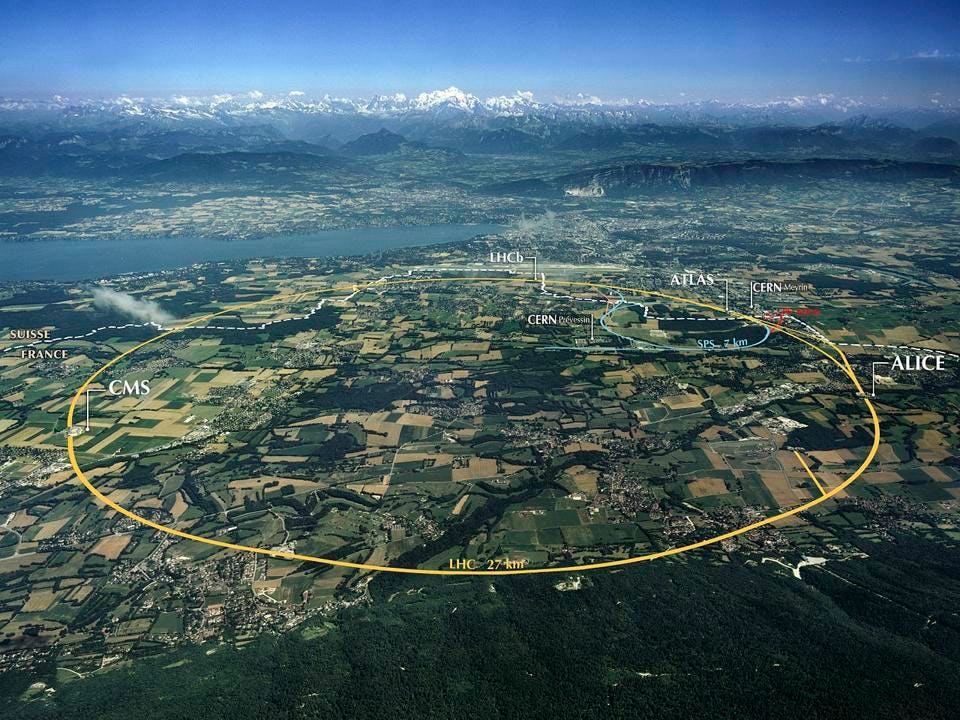
\includegraphics[width=0.75\textwidth,clip] {LHCaerial.jpg}
        \caption{An aerial view of CERN and the LHC, located near Geneva on the border between France and Switzerland.}
        \label{fig:LHCaerial}
    \end{center}
\end{figure}

Geological considerations dictated the placement of the tunnel at an average depth of 100 m, with variations ranging from 175 m beneath the Jura Mountains to 50 m near Lake Geneva. The tunnel follows a gentle gradient of 1.4\% to accommodate geological stability and minimize excavation costs. The location was also chosen to ensure minimal disruption to surface infrastructure and avoid heavily populated areas while maintaining proximity to CERN's primary research facilities.

\begin{table}[]
    \centering
    \begin{tabular}{|l|l|}
    \hline
    Design Parameter                & Value                                                                           \\ \hline
    Circumference                   & 26659 m                                                                        \\
    Dipole operating temperature    & 1.9 K (-271.3 ºC)                                                               \\
    Number of magnets               & 9593                                                                            \\
    Number of main dipoles          & 1232                                                                            \\
    Number of main quadrupoles      & 392                                                                             \\
    Number of RF cavities           & 8 per direction                                                                 \\
    Energy, protons                 & 7 TeV                                                                           \\
    Energy, ions                    & 2.76 TeV/u                                                                      \\
    Peak magnetic dipole field      & 8.3 T                                                                           \\
    Distance between bunches        & $\sim$7.5 m                                                                     \\
    Luminosity (protons)            & $10^{34} cm^{-2} s^{-1}$ \\
    No. of bunches per proton beam  & 2808                                                                            \\
    No. of protons per bunch        & 1.1 x 1011                                                                      \\
    Number of turns per second      & 11245                                                                           \\
    Number of collisions per second & 1 billion                                                                       \\ \hline
    \end{tabular}
    \caption{Design parameters for the LHC~\cite{CERNBroc79}}
    \label{tab:LHCparam}
\end{table}

The LHC relies on superconducting electromagnets to maintain and guide the circulating beams. Specifically, 1232 dipole magnets, each measuring 15 meters in length, generate a magnetic field of 8.3 T to bend the trajectory of the protons. These dipoles, along with 392 quadrupole magnets (each between 5 and 7 meters long) responsible for beam focusing, are composed of niobium-titanium (NbTi) superconducting cables. These materials exhibit superconductivity below 10 K (-263.2$^{\circ}$C), though the LHC operates at an even lower temperature of 1.9 K (-271.3$^{\circ}$C). The ultrahigh vacuum maintained within the beam pipes ($10^{-10}$ to $10^{-11}$ mbar) is colder than the cosmic microwave background temperature (2.7 K) and approaches the surface pressure of the Moon. 

This extreme cooling is necessary to ensure minimal resistance in the superconducting magnets and to reduce unwanted interactions that could degrade beam quality. To sustain these cryogenic conditions, the LHC employs 96 tonnes of superfluid helium, making it the world’s largest cryogenic system. Beam control and stability are further enhanced by specialized multipole magnets and final focusing quadrupoles near interaction points. Prior to collision, the beams undergo final focusing, compressing their transverse size to maximize interaction probability. The precision required for this process is akin to aligning two needles 10 km apart such that they collide at their midpoint. 

All accelerator operations, including beam injection, acceleration, steering, and diagnostics, are centrally coordinated from the CERN Control Center. The LHC facilitates collisions at four primary interaction regions housing major particle detectors: ATLAS (A Toroidal LHC ApparatuS), CMS (Compact Muon Solenoid), ALICE (A Large Ion Collider Experiment), and LHCb (Large Hadron Collider beauty). Of these, ATLAS and CMS serve as general-purpose detectors, while LHCb specializes in flavor physics, particularly the study of b-quarks, and ALICE investigates heavy-ion collisions. Each of these experiments has dedicated research objectives, with ATLAS and CMS playing a central role in Higgs boson studies and searches for BSM physics, while ALICE focuses on recreating conditions similar to those moments after the Big Bang, such as with quark-gluon plasmas. This thesis presents results obtained using pp collision data recorded by the CMS experiment.

Proton beams at the LHC are structured into well-defined bunches due to the constraints imposed by RF acceleration. Under nominal conditions, each beam comprises 2808 bunches, with each bunch containing approximately $10^{11}$ protons. Given the minute transverse dimensions of the bunches, the probability of individual proton-proton collisions becomes very large through the high luminosity achieved through intense beam focusing and bunch structuring. At each interaction point, up to 60 simultaneous collisions can occur per bunch crossing. With bunch crossings occurring at a rate of $\sim40$ MHz, the LHC generates approximately $2.5 \times 10^9$ proton-proton interactions per second. This vast amount of data necessitates sophisticated triggering systems to selectively record the most interesting events while discarding redundant or low-energy interactions. Advances in machine learning techniques have also been integrated into the LHC's data-processing pipeline to optimize event selection and improve detection of rare physics processes.

A key parameter quantifying collider performance is luminosity, defined as the number of interactions per unit area per unit time. While luminosity at the LHC is often reported integrated over a period of active beam, the instantaneous luminosity can be calculated in terms of the accelerator parameters as follows:

\begin{equation}
\label{eq:lumi}
\begin{gathered}
\mathcal{L} = \frac{\gamma f N_p^2 N_b}{4 \pi \epsilon_n \beta^*} \mathcal{F}
\end{gathered}
\end{equation}

where $N_p$ is the number of particles per bunch, $N_b$ is the number of bunches per beam, $f$ is the revolution frequency of the bunches around the ring, $\epsilon_n$ is the transverse emittance, $\beta^*$ is the amplitude function at the interaction or crossing point, $\mathcal{F}$ is a geometric factor correlated to the crossing angle of the beams, and $\gamma$ is the relativistic Lorentz factor $\frac{1}{\sqrt{1-\beta^2}}$. A plot of the integrated luminosities delivered and recorded by CMS is shown in Figure~\ref{fig:cmsintlumi}. This thesis includes data through 2018 (Run 1 + Run 2).

The number of events for a particular interaction also depends on its probability, expressed as a cross section in units of area. When investigating a specific physics process, the event rate is determined by the product of the luminosity ($\mathcal{L}$) and the process-specific cross-section ($\sigma$):

\begin{equation}
\label{eq:crosssection}
\begin{gathered}
\frac{dN}{dt} = \mathcal{L} \times \sigma.
\end{gathered}
\end{equation}

\begin{figure}[!hbt]
\begin{center}
    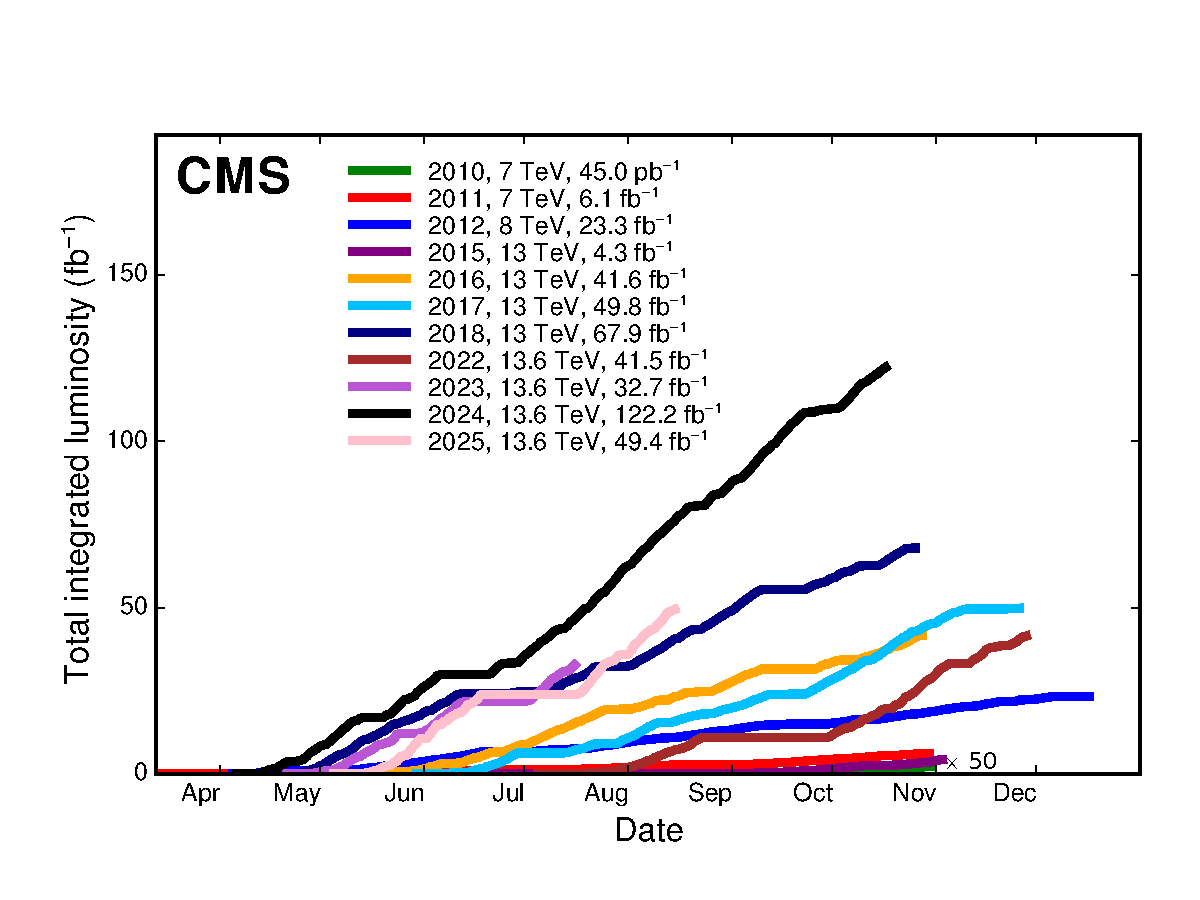
\includegraphics[width=0.8\textwidth,clip] {int_lumi_cumulative_pp_2.pdf}
    \caption{Cumulative luminosity versus day delivered to CMS during stable beams for pp collisions at nominal center-of-mass energy. This is shown for data-taking in 2010 (green), 2011 (red), 2012 (blue), 2015 (purple), 2016 (orange), 2017 (light blue), 2018 (navy blue), 2022 (brown), and 2023 (light purple). These plots use the best available offline calibrations for each year.}
    \label{fig:cmsintlumi}
\end{center}
\end{figure}

\section{The Compact Muon Solenoid} \label{chap:chap-3.2-CMS}
The CMS detector is built around a large superconducting solenoid, for which it is named. It spans 6 meters in its internal diameter and generates a magnetic field of 3.8 Tesla. This very large field bends the trajectories of charged particles which helps to identify their momenta along with charge information. Inside the solenoid we find silicon trackers and calorimeters, while outside the solenoid we have layers of muon detection chambers \cite{CMStechprop, The_CMS_Collaboration_2008, Contardo:2020886}.

\begin{figure}[!hbt]
\begin{center}
    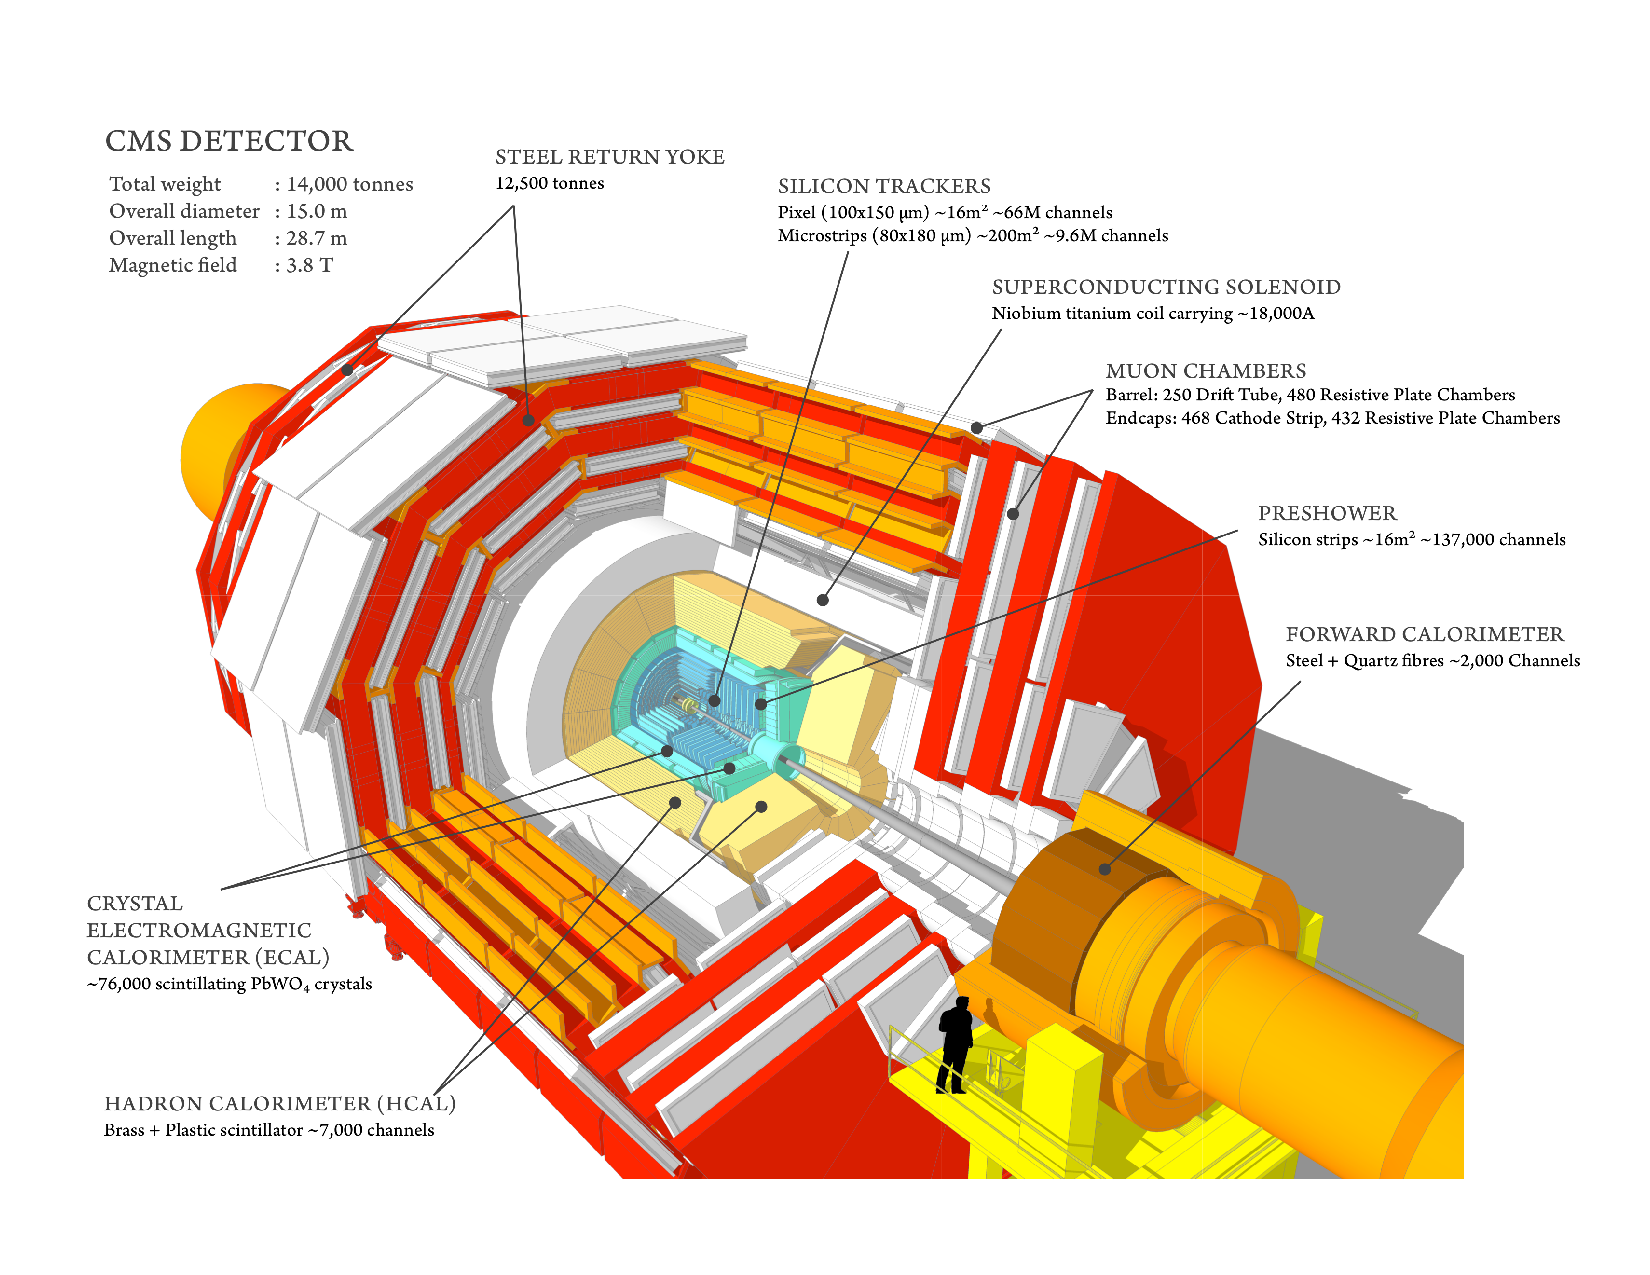
\includegraphics[width=0.8\textwidth,clip] {cmsdetector.pdf}
    \caption{The CMS detector is shaped like a cylindrical onion, with several concentric layers of components.}
    \label{fig:cmscutaway1}
\end{center}
\end{figure}

A useful analogy is that CMS effectively acts like a high-speed camera, taking 3-dimensional ``snapshots'' of particle collision events in all directions up to 40 million times each second. Although most of the initial collision products decay rapidly, the stable products can be detected by CMS as they travel away from the beamline. By identifying the stable particles produced in each collision and then piecing them together, the detector can reconstruct an understanding of the collision which can then be analyzed to identify constituent physics phenomena \cite{Karimaki:368412, CERN-LHCC-2000-016, Chatrchyan:1129810, Collaboration:2745805, CERN-LHCC-2017-009}.

\subsection{Solenoid}
The eponymous superconducting solenoid is central to the construction and operation of CMS, and features an internal diameter of 6 m. As the largest superconducting magnet ever built, its coils and return yoke weigh in at 12,500 tonnes and it is cooled to 1.9 K ($-268.5^\circ$C), approaching the temperature of deep space. It also generates a uniform magnetic field of 3.8 T, which is approximately $10^5$ times stronger than the Earth's magnetic field.

\begin{figure}[!hbt]
    \begin{center}
        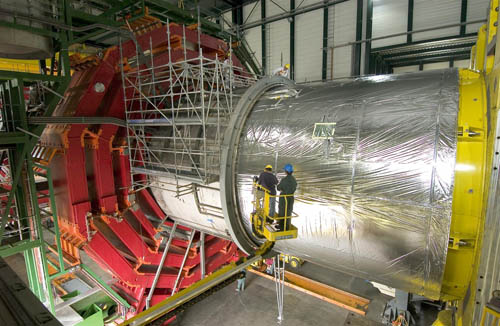
\includegraphics[width=0.75\textwidth,clip] {CMSmagnet.jpg}
        \caption{View of the CMS magnet during construction.}
        \label{fig:CMSmagnet}
    \end{center}
\end{figure}

This intense field bends the trajectories of charged particles produced in high-energy collisions. The degree of deflection is inversely proportional to a particle’s momentum, allowing precise momentum measurements through high-resolution tracking in conjunction with the well-calibrated magnetic field. High-energy particles exhibit minimal curvature, necessitating exceptional spatial resolution to accurately reconstruct their momenta. This motivates the precise alignment of the tracker in CMS. 

\begin{figure}[!hbt]
    \begin{center}
        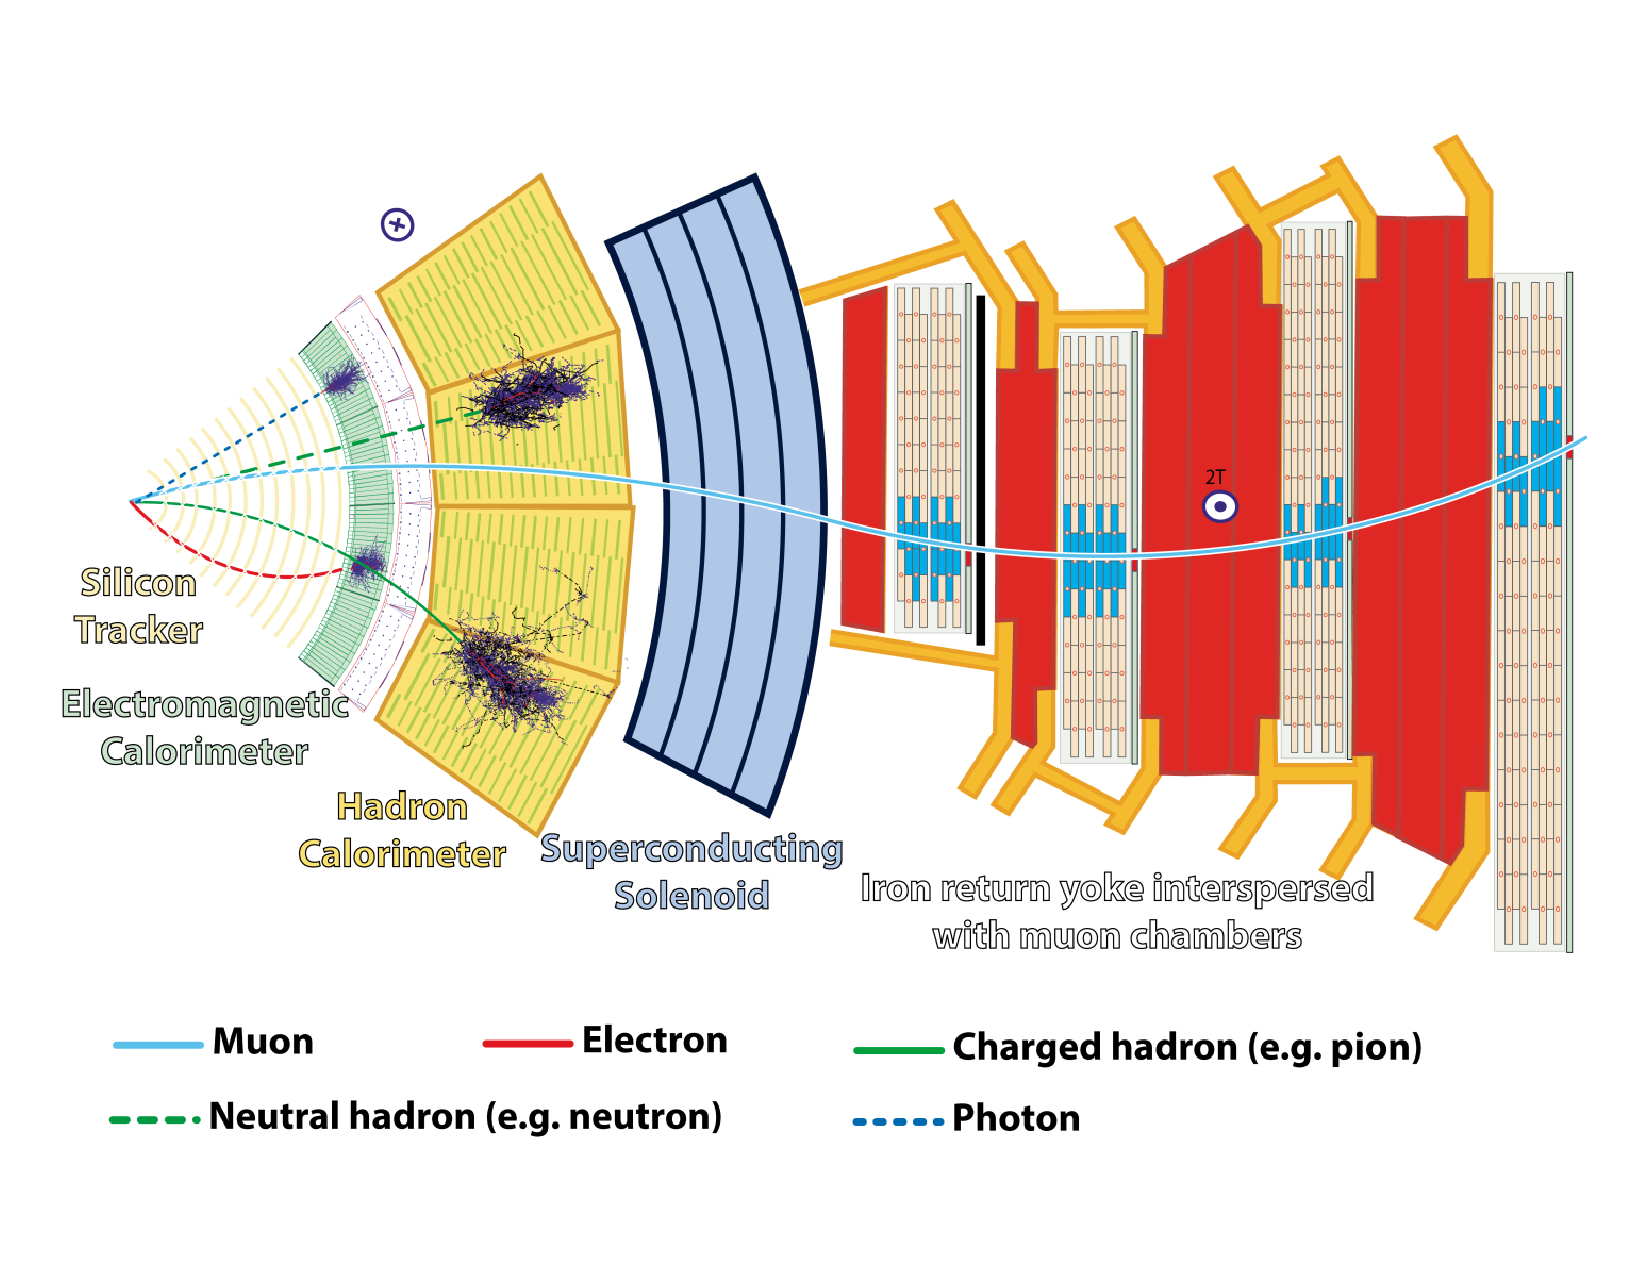
\includegraphics[width=0.8\textwidth,clip] {CMSslice.pdf}
        \caption{Schematic view of the CMS detector.}
        \label{fig:cmscutaway2}
    \end{center}
\end{figure}

The inner tracking system and electromagnetic and hadronic calorimeters (ECAL and HCAL) are housed within the solenoid coil. The solenoid itself provides primary structural support for the CMS experiment, and is robustly engineered to withstand the immense forces generated by its own magnetic field. Surrounding the solenoid is a 12-sided iron return yoke, which integrates the muon detection system and serves to contain and guide the magnetic field. Comprising of three layers, the yoke extends to a diameter of 14 m and functions as a physical filter, allowing only muons and weakly interacting particles, such as neutrinos, to pass through. 

\subsection{Silicon Tracker}

The CMS tracker is designed to precisely record charged particle trajectories while minimizing material interactions to reduce additional scattering and energy loss. This is achieved through high-precision spatial measurements, enabling accurate track reconstruction with a minimal number of data points. Each position measurement is recorded with a resolution of $\sim10$ $\mu$m, an order of magnitude smaller than the width of a human hair, ensuring precise momentum determination.

As the innermost subsystem of CMS, the tracker operates in a highly irradiated environment due to its proximity to the interaction point. Consequently, its construction materials were meticulously selected for radiation hardness to maintain performance.

\begin{figure}[!hbt]
    \begin{center}
        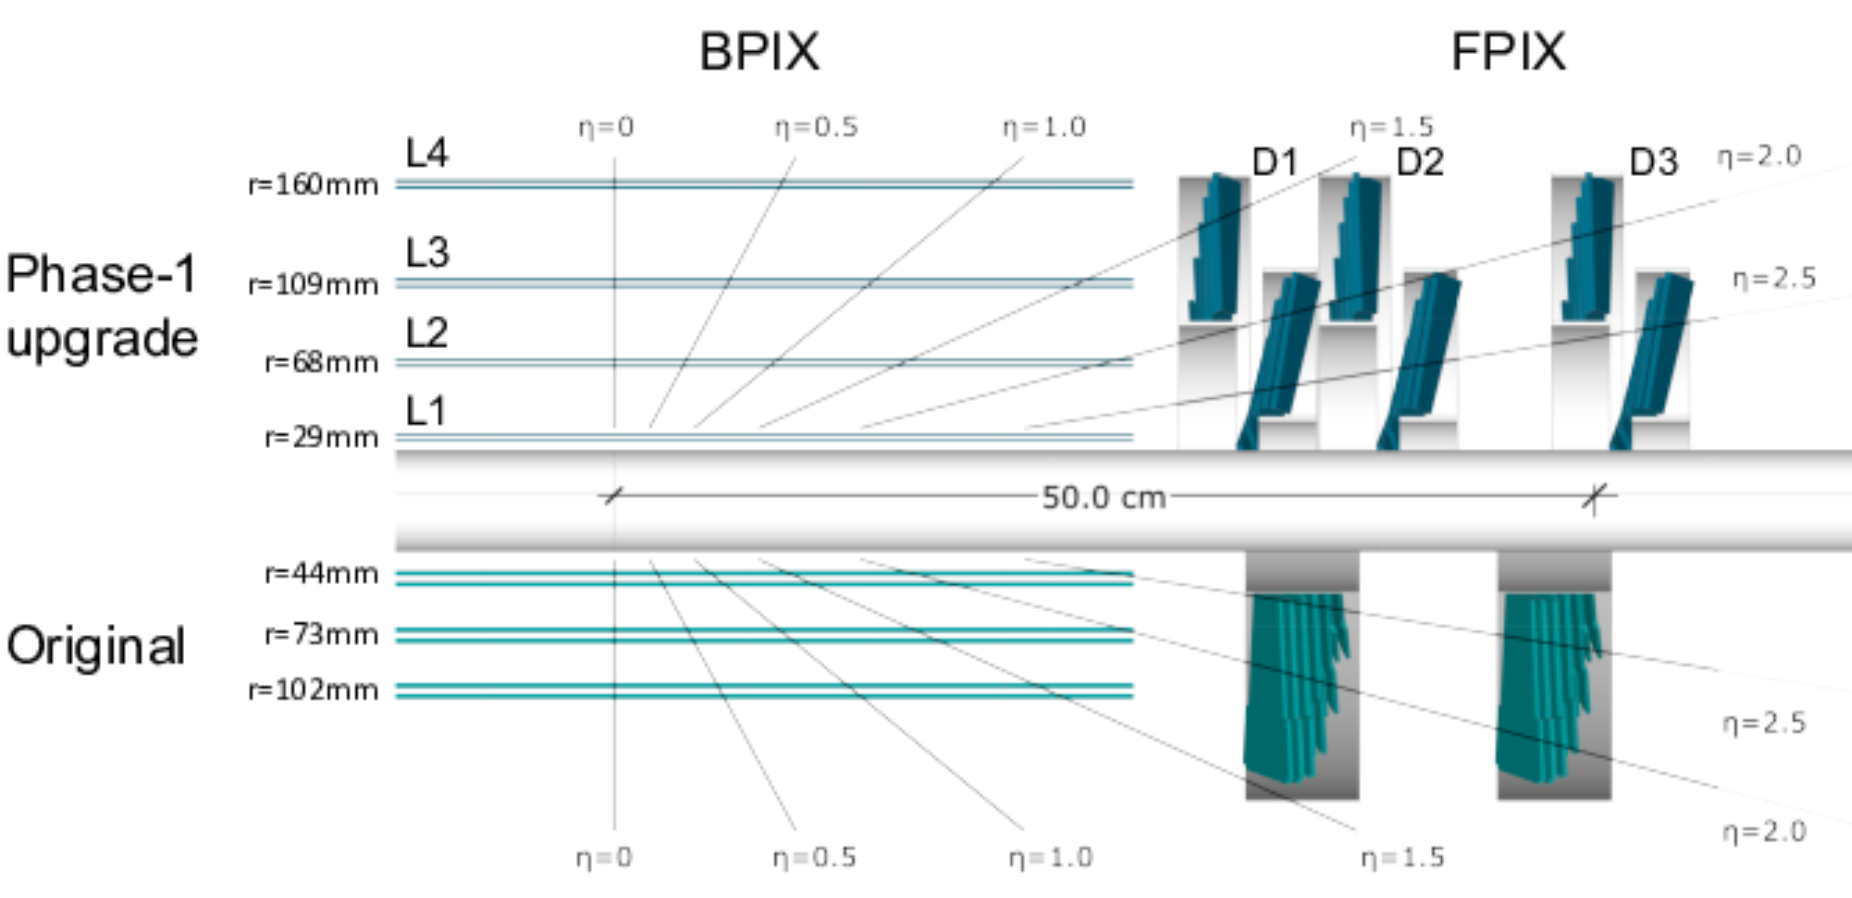
\includegraphics[width=0.75\textwidth,clip] {TrackerLayoutWithLAS2.png}
        \caption{Illustration of the differences between the original design of the silicon tracker and the Phase-1 upgrade~\cite{Adam:2748381, Collaboration:1355706, CMS:2012sda}. This thesis utilized data from LHC Run 2 after the Phase-1 upgrades to the tracker.}
        \label{fig:silicontracker}
    \end{center}
\end{figure}

\begin{figure}[!ht]
    \begin{center}
        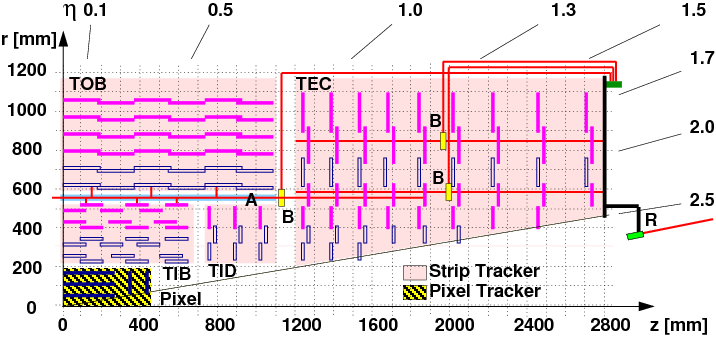
\includegraphics[width=0.8\textwidth,clip] {TrackerLayoutWithLAS.png}
        \caption{Schematic view of one quarter of the tracker in the r-z plane. This details the full silicon detector with all modules in their original positions.}
        \label{fig:silicontracker2}
    \end{center}
\end{figure}

A cross sectional view of the CMS tracker is shown in Figures~\ref{fig:silicontracker}~and~\ref{fig:silicontracker2}. The tracker is composed of multiple silicon-based detector layers optimized for spatial resolution and radiation tolerance. It consists of two pixel subdetectors, the Tracker Pixel Barrel (TPB) and Tracker Pixel Endcap (TPE), which provide the highest granularity near the beamline. Beyond the pixel detectors, four silicon strip subdetectors extend tracking coverage: the Tracker Inner Barrel (TIB) and Tracker Inner Disks (TID) provide intermediate precision measurements, while the Tracker Outer Barrel (TOB) and Tracker Endcap (TEC) contribute to tracking particles at larger radii from the collision point~\cite{Chatrchyan:1667597}. 

% The tracker must precisely record particle paths while remaining lightweight to minimize interference with the particles. 
% It achieves this by capturing highly accurate position measurements, allowing tracks to be reliably reconstructed with only a few data points. 
% Each measurement has an accuracy of 10 µm, which is a fraction of the width of a human hair. 
% As the innermost component of the CMS detector, the tracker is exposed to the highest volume of particles, so its construction materials were carefully selected for radiation resistance.

% The tracker is assembled from several distinct detector elements, consisting of two silicon pixel subdetectors, the Tracker Pixel Barrel (TPB) and Tracker Pixel Endcap (TPE); 
% and four silicon strip subdetectors, the Tracker Outer Barrel (TOB), Tracker Inner Barrel (TIB), Tracker Inner Disks (TID), and Tracker Endcap (TEC) \cite{Chatrchyan:1667597}.

\subsubsection{Pixel Detector}

The CMS pixel detector (a photograph of which is presented in Figure~\ref{fig:CMSpixel}) contains an array of 124 million pixels and is positioned closest to the beam pipe, which makes it essential for reconstructing the short-lived decay products of heavy particles. In the Phase-1 geometry, the pixel detector consists of four cylindrical barrel (BPIX) layers located at radii of approximately 3~cm, 7~cm, 11~cm, and 16~cm, with additional forward and backward endcap disks (FPIX) extending coverage at angles along the beamline (regions with higher values of pseudorapidity, parameterized by $\eta$ as seen in Figures~\ref{fig:silicontracker}~and~\ref{fig:silicontracker2}).

\begin{figure}[!hbt]
    \begin{center}
        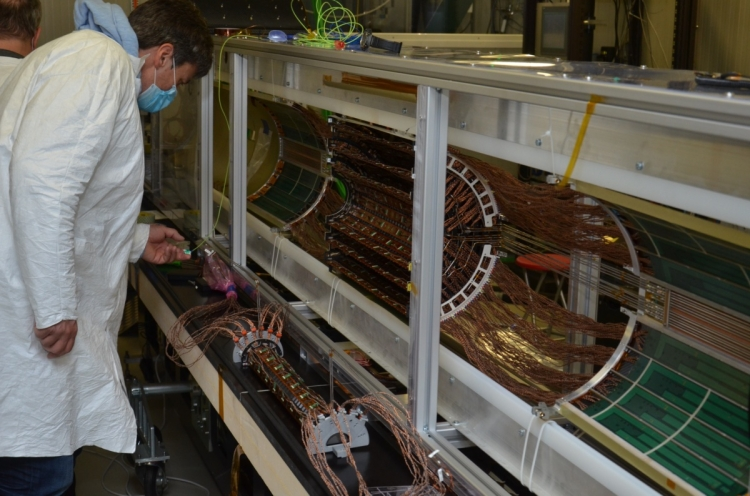
\includegraphics[width=0.65\textwidth,clip] {CMSpixel.jpg}
        \caption{Silicon pixel detector before installation.}
        \label{fig:CMSpixel}
    \end{center}
\end{figure}

Each of the four layers is composed of silicon sensor modules, subdivided into individual pixels as visualized in Figure~\ref{fig:Pixelement}. Each pixel measures 100~$\mu$m $\times$ 150~$\mu$m, comparable to the width of two human hairs. When a charged particle traverses a pixel sensor, it ionizes the silicon atoms along its path, liberating electron-hole pairs. A bias voltage applied across the sensor collects these charges, generating a small electric signal. This signal is subsequently amplified and processed by an electronic readout chip, with each module integrating 16 readout chips (ROCs) to handle data acquisition efficiently. Given the detector’s close proximity to the beamline, the particle flux is extreme, reaching approximately $6 \times 10^8$ particles per cm$^2$ per second at a radius of 3~cm~\cite{The_CMS_Collaboration_2008}.

\begin{figure}[!hbt]
    \begin{center}
        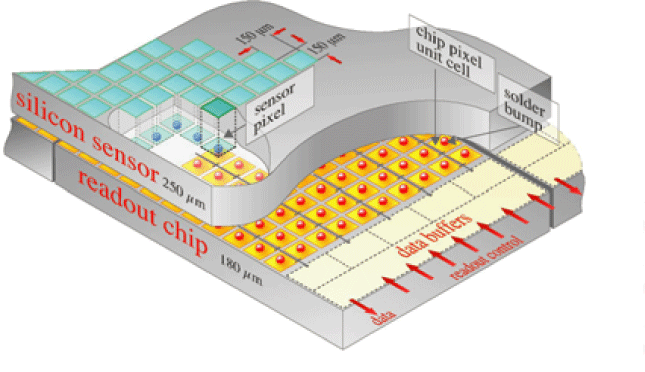
\includegraphics[width=0.75\textwidth,clip] {Pixelement.png}
        \caption{Illustration of the CMS silicon sensor modules.}
        \label{fig:Pixelement}
    \end{center}
\end{figure}

% The pixel detector, despite being only about the size of a shoebox, contains 124 million pixels, enabling it to track particle paths with exceptional accuracy as they emerge from collisions. 
% Positioned closest to the beam pipe, it features cylindrical layers located approximately at radii of 3 cm, 7 cm, 11 cm, and 16 cm, with disks at either end. 
% This proximity makes the pixel detector crucial for reconstructing the tracks of very short-lived particles.

% Each of the four layers is composed of individual silicon modules, split into numerous pixels. Each of these silicon pixels is 100µm by 150µm, about the width of two human hairs. 
% When a charged particle passes through a pixel, it ejects electrons from the silicon atoms. A voltage applied to the sensor allows the collection of these charges as a small electric signal, which is then amplified by an electronic readout chip (with a total of 16 chips per module). This design allows for significant bandwidth from the pixel detector, which is necessitated by the proximity to the point of collisions. The rate of particles received at 3 cm from the beamline is around 600 million particles per square centimeter per second.

% Knowing which pixels have been energized allows us to deduce the particle's trajectory. And because the detector has 124 million of these pixels, arranged in four stacked layers of silicon modules, we can create a three-dimensional picture of each particle's path.

\subsubsection{Strip Detector}

After passing through the pixel detector, charged particles traverse ten successive layers of silicon strip detectors, extending the tracking coverage to a radius of 130~cm. These layers provide high-precision position measurements over a larger volume, complementing the pixel detector in track reconstruction, particularly for higher-momentum particles that travel greater distances before bending significantly in the magnetic field~\cite{Chatrchyan:1667597}. A diagram and photograph of the strip layers are presented in Figures~\ref{fig:CMSBarrel}~and~\ref{fig:CMStracker}, respectively. 

\begin{figure}[!hbt]
    \begin{center}
        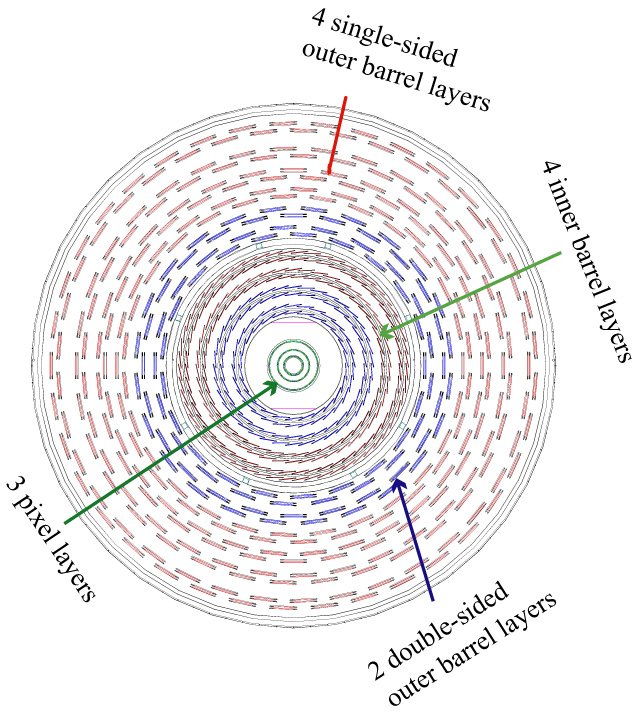
\includegraphics[width=0.6\textwidth,clip] {CMSBarrel.png}
        \caption{CMS Tracker layers shown in the plane perpendicular to the beam.}
        \label{fig:CMSBarrel}
    \end{center}
\end{figure}

The silicon strip tracking system consists of multiple subdetectors, each optimized for its position within the detector. The inner tracking volume comprises the Tracker Inner Barrel (TIB), composed of four concentric layers, and the Tracker Inner Disks (TID), each consisting of three small disk-shaped structures. Encasing the TIB and TID is the Tracker Outer Barrel (TOB), which consists of six additional layers, providing extended coverage in the barrel region. At both ends of the tracker, the Tracker Endcaps (TEC) ensure full pseudorapidity coverage. The geometries of these subsystems are carefully optimized to balance spatial resolution, material budget, and mechanical stability~\cite{CMS:trackerTDR}. 

\begin{figure}[!hbt]
    \begin{center}
        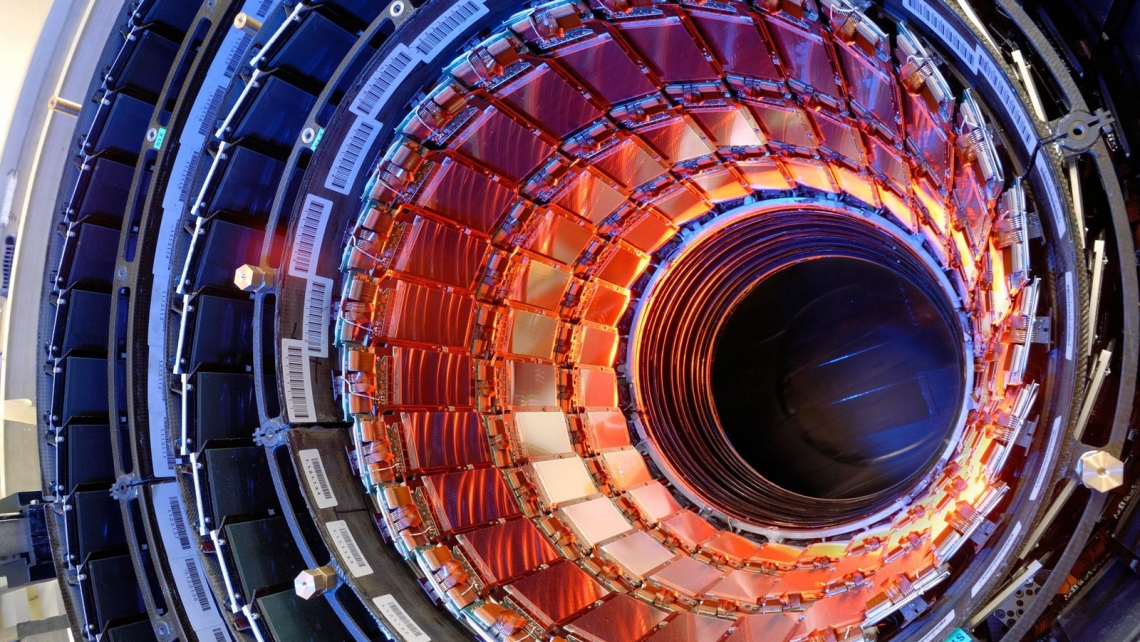
\includegraphics[width=0.65\textwidth,clip] {CMStracker.jpg}
        \caption{Photograph of the silicon strip detectors in the barrel module.}
        \label{fig:CMStracker}
    \end{center}
\end{figure}

The silicon strip tracker contains a total of 15,200 highly sensitive modules, comprising approximately 10 million detector strips read out by 72,000 microelectronic chips. Each module consists of three primary components: one or two silicon strip sensors, a mechanical support structure ensuring precise alignment and stability, and readout electronics responsible for amplifying and processing signals. This extensive system enables precise tracking of charged particles throughout their passage within the CMS detector, ensuring robust vertex reconstruction and momentum measurements~\cite{CMS:trackingPerf}.

% After traversing the pixel detectors, particles move through ten layers of silicon strip detectors, which extend to a radius of 130 centimeters.

% The silicon strip detector is composed of four inner barrel (TIB) layers and two inner endcaps (TID), each made up of three small discs. Surrounding both the TIB and TID is the outer barrel (TOB), consisting of six concentric layers. At either end of the tracker, two endcaps (TEC) provide closure. Each of these components contains silicon modules, wtih geometries optimized for their specific location within the detector.

% This section of the tracker contains 15,200 highly sensitive modules, with a total of approximately 10 million detector strips read by 72,000 microelectronic chips. Each module comprises three main elements: one or two silicon sensors, a mechanical support structure, and readout electronics.

\subsection{Electromagnetic Calorimeter}

The ECAL is the innermost of the two calorimeters in CMS and is designed to measure the energy of electrons and photons with high precision by fully absorbing them.

The ECAL houses approximately 80,000 lead tungstate (\(\text{PbWO}_4\)) crystals, a scintillating material selected for its high density (\(\rho = 8.28 \, \text{g/cm}^3\)), short radiation length (\(X_0 = 0.89 \, \text{cm}\)), and fast response time. Each crystal, primarily composed of lead bound with oxygen in a tungstate lattice structure, took two days to grow and has a mass of 1.5 kg and is characterized by exceptional optical transparency despite its metallic composition. When traversed by high-energy electrons or photons, these crystals emit scintillation light in short, well-defined bursts, enabling precise energy measurements and particle identification. The ECAL barrel is shown in Figure~\ref{fig:ECAL}.

\begin{figure}[!hbt]
    \begin{center}
        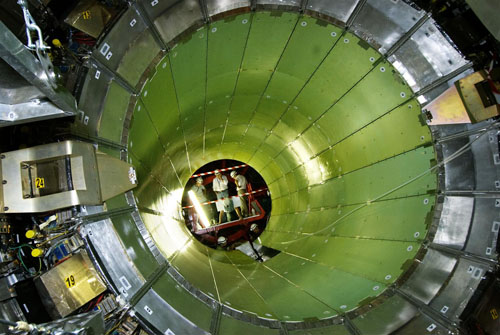
\includegraphics[width=0.65\textwidth,clip] {ECAL.jpg}
        \caption{Photograph of the CMS ECAL during construction.}
        \label{fig:ECAL}
    \end{center}
\end{figure}

The emitted scintillation light is detected by photodetectors, specifically avalanche photodiodes (APDs) in the barrel region and vacuum phototriodes (VPTs) in the endcaps. These photodetectors convert the optical signal into an electrical signal, which is then amplified and digitized for precise energy reconstruction. The ECAL’s excellent energy resolution (\(\sim1\%\) at 100 GeV) for high-energy electrons and photons makes it a critical component for the identification of physics phenomena such as Higgs boson decays and precision Standard Model measurements~\cite{CMS:ECALPerf, CMS:ECALTDR, CMS:JINST}.

% The Electromagnetic Calorimeter (ECAL) is the inner layer of the two calorimeters and measures the energy of electrons and photons by stopping them completely. 

% The ECAL is constructed using nearly 80000 lead tungstate crystals, which are made primarily of metal (bound with oxygen in this crystalline form) and each weigh 1.5 kg. These crystals are incredibly dense yet highly transparent, and scintillate when electrons and photons pass through them. The light is produced in short, well-defined photon bursts which allows for precise identifications of the passing charged particles.

\subsection{Hadron Calorimeter}

Hadrons, composite particles composed of quarks and gluons bound by the strong interaction, pass through the ECAL with minimal energy deposition before being absorbed in the HCAL~\cite{CERN-LHCC-97-031, Mans:1481837}. A photograph of the HCAL barrel is shown in Figure~\ref{fig:HCAL}.

The HCAL is designed to measure the energy, position, and timing of hadronic showers. It consists of alternating layers of dense absorber material (brass and steel plates), which induces hadronic interactions, and flourescent scintillator tiles, which produce optical signals proportional to the deposited energy. These scintillation signals are collected via wavelength-shifting fibers and transmitted to hybrid photodiodes (HPDs) for digitization~\cite{CERN-LHCC-97-031, Mans:1481837}. The absorber material is critical, as hadronic interactions necessitate a substantial thickness---material of $\sim$5.82 nuclear interaction lengths in the barrel region and $\sim$10 nuclear interaction lengths along the beam---to ensure full shower containment~\cite{CERN-LHCC-97-031, Mans:1481837}.

\begin{figure}[!hbt]
    \begin{center}
        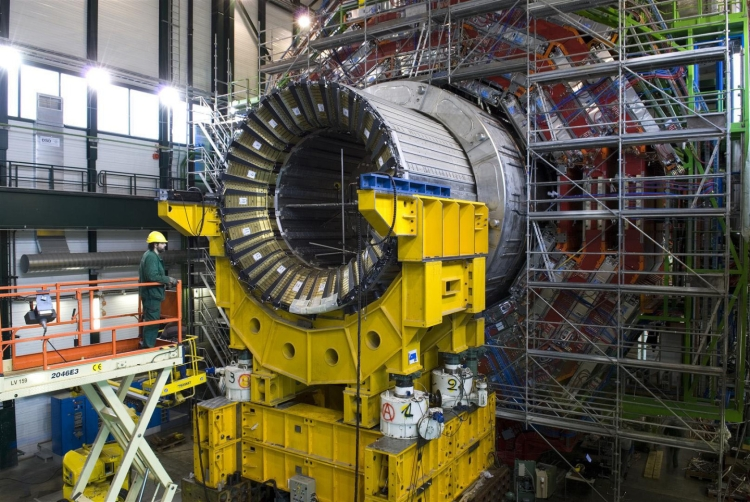
\includegraphics[width=0.65\textwidth,clip] {HCAL.jpg}
        \caption{Insertion of the HCAL barrel inside the magnet in 2008.}
        \label{fig:HCAL}
    \end{center}
\end{figure}

The HCAL is structured into four primary components: the Hadron Barrel (HB), the Hadron Outer (HO), the Hadron Endcap (HE), and the Hadronic Forward (HF) calorimeters. The HB and HE employ brass absorber plates interleaved with plastic scintillator tiles, selected for their balance between density and cost-effectiveness. The HO, positioned outside the superconducting solenoid, captures late-developing showers that might otherwise escape detection. The HF, located at high pseudorapidity (\(\eta\)), utilizes quartz fibers embedded in a steel absorber, leveraging Cherenkov light production to make measurements in the forward region~\cite{CMS-HCAL-Performance}.

The HE calorimeters consist of 36 wedge-shaped modules, covering the pseudorapidity range \(1.3 < |\eta| < 3.0\), extending hadronic energy measurements beyond the barrel region. The HF calorimeters, spanning \(3.0 < |\eta| < 5.2\), play a crucial role in detecting forward jets and reconstructing missing transverse energy (\(E_T^{\text{miss}}\)), which is essential for identifying weakly interacting particles such as neutrinos or potential BSM candidates~\cite{CMS-Trigger-Performance}.

% Hadrons, which are composite particles made up of quarks and gluons, fly through the ECAL and are stopped by the outer layer called the Hadron Calorimeter (HCAL) \cite{CERN-LHCC-97-031}.

% The HCAL is a sampling calorimeter meaning it finds a particle’s position, energy, and arrival time using alternating layers of dense ``absorber'' and fluorescent ``scintillator'' materials that produce a rapid light pulse when the particle passes through. Fitting the HCAL into the ``compact'' CMS required the use of very densely packed materials and geometry, since the minimum amount of material needed to contain and measure a hadron's shower is about one meter. 

% To accomplish this feat, the HCAL is organised into barrel (HB and HO), endcap (HE), and forward (HF) sections. The endcaps are constructed from 36 ``wedges'' which measure particle energies as they emerge through the ends of the solenoid magnet. In addition, there are 36 barrel pieces, each weighing 26 tonnes, around the circumference of the barrel. These form the last layer of detectors inside CMS's magnet coil, since the outer barrel (HO) sits outside the coil to ensure that no energy escapes CMS undetected. 

% Finally, the two hadronic forward calorimeters (HF) are positioned at either end of the detector, to capture any particles coming out of the collision region at large $\eta$, or shallow angles relative to the beam line. These receive the bulk of the energy from the particle collisions, so the HFs are very radiation hard.

\subsection{Muon System}

The detection of muons is one of the primary objectives of the CMS experiment\footnote{While we depend on our detection of electrons too, muons are more difficult to capture and measure, so we will focus on them here.}. Muons are charged leptons, similar to electrons and positrons, but approximately 200 times heavier. This increased mass grants them a significantly greater penetration depth because it reduces the energy lost by the traveling particles through various mechanisms, allowing them to traverse several meters of material with minimal energy loss. Unlike most particles produced in high-energy collisions, muons are not fully absorbed by the electromagnetic (ECAL) or hadronic (HCAL) calorimeters. Consequently, dedicated muon detection chambers are positioned in the outermost regions of CMS, beyond the solenoid magnet, where muons are often the only particles producing a distinct and measurable signal.

The CMS muon system consists of four muon stations, which are interleaved with the iron plates of the return yoke. The system incorporates 1400 muon chambers, comprising 250 drift tubes (DTs) and 540 cathode strip chambers (CSCs) responsible for tracking and triggering, along with 610 resistive plate chambers (RPCs) and 72 gas electron multiplier chambers (GEMs), which provide a redundant trigger to ensure rapid data acquisition and filtering.

Muon tracking is performed by reconstructing the curvature of muon trajectories within the $3.8\,\mathrm{T}$ magnetic field generated by the CMS solenoid, as illustrated in Figure~\ref{fig:cmscutaway2} and Figure~\ref{fig:MuStations}. The reconstruction of muon momentum is achieved through a combination of measurements from the muon chambers, which provide track trajectory information, and the silicon tracker, which offers high-precision tracking near the interaction point. The combined resolution for transverse momentum measurements (\( p_T \)) is approximately 3--5\% for \( p_T > 10 \) GeV/\( c \).

\begin{figure}[!hbt]
\centering
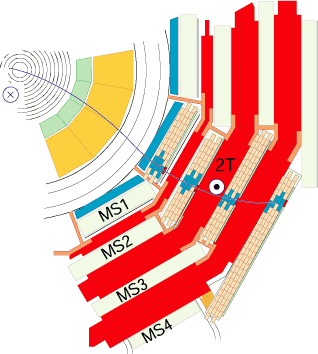
\includegraphics[width=0.50\textwidth]{figures/MuStations.png}
\caption{A muon, in the plane perpendicular to the LHC beams, leaves a curved trajectory in four layers of  muon ``stations.'' Note that the muon passes through the silicon tracker first, which measures momentum, charge, trajectory, and impact parameter, or how close the muon's path is to the primary vertex.}
\label{fig:MuStations}
\end{figure}    

At low transverse momentum (\( p_T < 200 \) GeV/\( c \)), the resolution of the muon system is primarily limited by multiple scattering effects in the material preceding the muon stations. However, at high transverse momentum (\( p_T > 200 \) GeV/\( c \)), the dominant limiting factor is the intrinsic spatial resolution of the muon chambers. The highest precision for low-momentum muons is obtained from the inner tracker alone, while for higher momentum muons, optimal resolution is achieved by combining measurements from both the muon system and the silicon tracker.

Accurate tracking requires precise alignment of the muon chambers and silicon tracker, which is achieved through cosmic ray data and dedicated calibration runs, ensuring sub-millimeter alignment precision. Each detector type undergoes rigorous calibration procedures to maintain accurate timing and spatial measurements. This includes gas gain calibration for the DT and CSC chambers, as well as timing calibrations for the RPC chambers. Overall, the CMS muon system is able to achieve an efficiency exceeding 95\% for the detection of high-momentum muons. 


% As its name suggests, detecting muons is one of the most important tasks of CMS. Muons are charged particles that are just like electrons and positrons, but 200 times heavier, and with much greater penetration depth. 
% Because they can travel through several meters of material without losing much energy, unlike most created particles, they are not stopped by any of CMS calorimeters. Therefore, chambers specifically designed to detect muons are placed in the outer part of CMS, where they are likely to be the only particles producing a clear signal.



% Muon hits are registered in the four muon stations, which are located outside of the magnet coil interleaved with the iron ``return yoke'' plates previously mentioned.

% In total there are 1400 muon chambers: 250 drift tubes (DTs) and 540 cathode strip chambers (CSCs) track the particle positions and provide a trigger, while 610 resistive plate chambers (RPCs) and 72 gas electron multiplier chambers (GEMs) form a redundant trigger system, which quickly decides to keep or discard the acquired muon data. 


% Muon tracking is achieved by measuring the curvature of muon trajectories in the $3.8\,\mathrm{T}$ magnetic field generated by the CMS solenoid.

% The muon momentum is reconstructed by combining data from The muon chambers (for trajectory information), and The silicon tracker (for high-precision tracking near the interaction point). The combined resolution is approximately $3$--$5\%$ for transverse momentum $p_T > 10\,\mathrm{GeV/c}$.

% The alignment of muon chambers is crucial for accurate tracking. Cosmic ray data and dedicated calibration runs are used to align the chambers to sub-millimeter precision.

% Each detector type undergoes gas and electronic calibration to ensure timing and spatial measurements are accurate. This process includes Gas gain calibration for DT and CSC chambers, and Timing calibration for RPC chambers.

% The muon system achieves $>95\%$ detection efficiency for high-momentum muons.
% It integrates seamlessly with the calorimeters, inner tracker, and solenoid to provide a complete picture of collision events.

\subsubsection{Muon Drift Tubes}

The drift tube (DT) system is responsible for tracking and identifying muons within the barrel region of the CMS detector. It detects charged particles as they pass through an array of gas-filled drift tubes. Each tube is a cylindrical chamber, 4 cm in width, containing a thin, positively charged anode wire aligned along its axis. The tubes are filled with a gas mixture, typically argon and carbon dioxide (CO$_2$), chosen to optimize ionization efficiency and ensure stable electron drift.

When a muon or any charged particle traverses a drift tube, it ionizes the gas atoms, liberating electrons. These electrons, guided by an applied electric field, drift toward the central anode wire, where they are amplified and produce a measurable charge pulse. The electron drift velocity within the gas mixture remains relatively constant, enabling precise determination of the particle’s trajectory. The time delay between ionization and signal detection provides an accurate measurement of the muon's crossing point within the drift cell.

Each DT chamber consists of multiple layers of staggered drift cells, grouped into units known as ``superlayers.'' Each superlayer contains four layers of drift tubes, offering redundant position measurements and improving spatial resolution. The DT system achieves a spatial resolution of approximately 1--2 mm, ensuring precise muon tracking.

The DT chambers are strategically positioned in the barrel region, covering a pseudorapidity range of $|\eta| < 1.2$. They are organized into four muon stations, which are embedded within the iron return yoke of the solenoid. The return yoke is structured into five wheels, each subdivided into twelve azimuthal sectors. Within this layout, each DT chamber is paired with one or two resistive plate chambers (RPCs), forming a complementary detection system that enhances muon identification and trigger efficiency.

A high-energy muon traversing the barrel region can interact with up to four DT chambers and six RPCs, resulting in as many as 44 recorded hits. This extensive tracking redundancy significantly improves momentum resolution and enhances robustness against inefficiencies in individual detectors. The DT system plays a crucial role in both tracking and triggering, delivering high-precision spatial and timing measurements that contribute to accurate muon momentum reconstruction~\cite{CMS:DTPerf, CMS:DTAlignment, CMS:MuonTDR}.

% \begin{figure}
% \centering
% 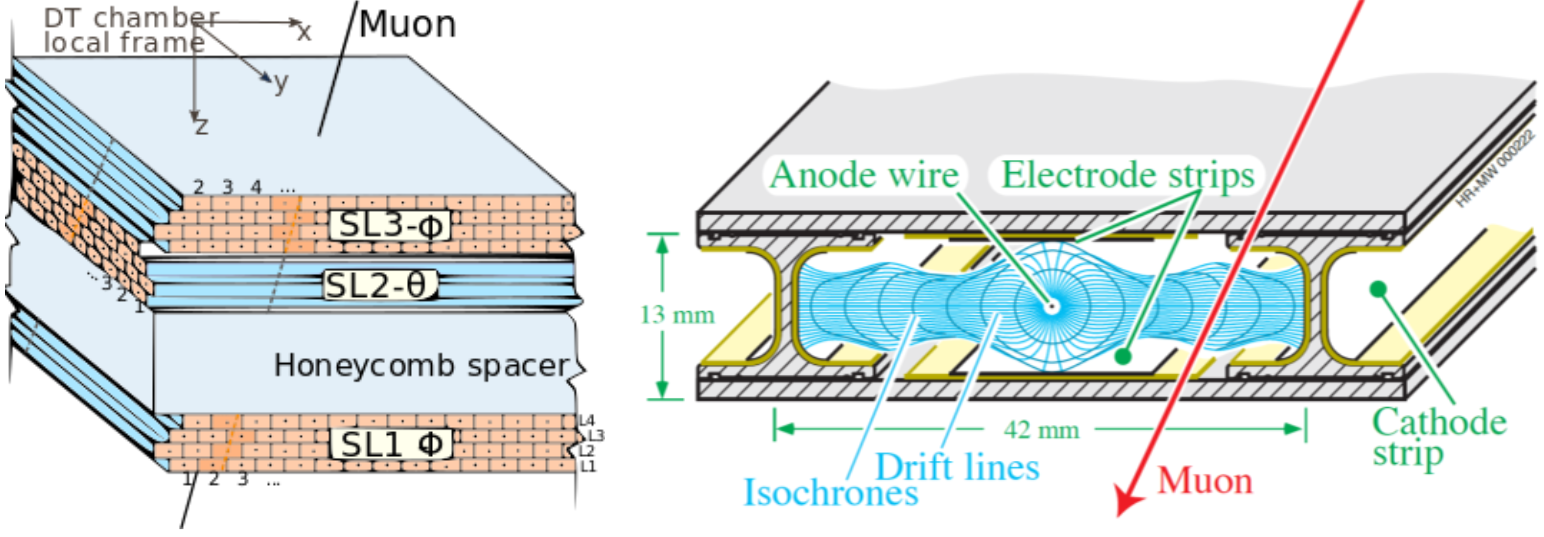
\includegraphics[width=0.60\textwidth]{figures/DTchambers.png}
% \caption{The sizes of DT chambers range from  2m x 2.5m to 4m x 2.5m, approximately.}
% \label{fig:DTchambers}
% \end{figure}    

% The drift tube (DT) system measures and identifies muon tracks in the barrel part of the detector. Each 4cm-wide tube contains a stretched wire within a gas volume. When a muon or any charged particle passes through the volume, it knocks electrons off the atoms of the gas. These electrons ``drift'' towards the anode following the electric field, ending up at the positively-charged wire where they are amplified and produce a measurable charge pulse. Each unit or ``superlayer'' contains four layers of staggered drift cells. By registering the time taken by the electrons to reach the wire, and since the drift velocity along the cell is a rather constant value, we can identify the exact crossing point of the muon along the cell.

% \begin{itemize}
% 	\item \textbf{Location:} DT chambers are located in the barrel region, covering a pseudorapidity range of $|\eta| < 1.2$.
% 	\item \textbf{Structure:} Each DT consists of parallel cylindrical drift tubes filled with a gas mixture, typically argon and carbon dioxide (CO$_2$).
% 	\item \textbf{Working Principle:} When a muon passes through a drift tube, it ionizes the gas. Electrons drift toward an anode wire under the influence of an electric field. The drift time provides precise position information.
% 	\item \textbf{Spatial Resolution:} Approximately $1$--$2\,\mathrm{mm}$.
% 	\item \textbf{Role:} DT chambers are used for both tracking and triggering, providing precise position and timing information.
% \end{itemize}

\subsubsection{Cathode strip chambers}

Cathode strip chambers (CSCs) are employed in the endcap disks, where the magnetic field is non-uniform, and particle fluxes are significantly higher than in the barrel region. These chambers are designed to provide precise muon tracking and triggering capabilities in this challenging environment. Each CSC consists of a multi-wire proportional chamber (MWPC) structure, comprising an array of positively charged anode wires intersecting with negatively charged copper cathode strips within a gas-filled chamber.

When a muon traverses a CSC, it ionizes the gas atoms, liberating electrons. These free electrons drift toward the anode wires under the influence of a strong electric field, initiating an avalanche multiplication process that results in a detectable charge pulse. Simultaneously, the positively charged ions drift toward the cathode strips, inducing a secondary charge signal. Since the anode wires are oriented perpendicularly to the cathode strips, the combined readout from both elements provides two-dimensional position information for the muon track.

CSCs are strategically positioned in the endcap regions, covering a pseudorapidity range of $1.2 < |\eta| < 2.4$. Each chamber consists of finely spaced cathode strips that enable high-resolution position measurements in the radial direction, achieving a spatial resolution of approximately 1 mm. The use of cathode strip readout, in conjunction with anode wire signals, allows for robust tracking and precise reconstruction of muon trajectories.

Given their location in the high-radiation forward region, CSCs play a crucial role in both muon tracking and triggering. They contribute significantly to the Level-1 (L1) trigger system, providing rapid and accurate muon identification to facilitate real-time event selection. Their ability to operate efficiently in regions with high background rates and strong magnetic field gradients makes them an essential component of the CMS muon detection system~\cite{CMS:MuonTDR, CMS_Collaboration_2010, Pozzobon:2701333}.


% \begin{figure}
% \centering
% 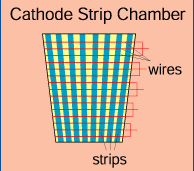
\includegraphics[width=0.50\textwidth]{figures/CSC.png}
% \caption{}
% \label{fig:CSC}
% \end{figure}    

% Cathode strip chambers (CSCs) are utilized in the endcap disks where the magnetic field is uneven, and particle rates are higher compared to the barrel. The chambers are made up of arrays of positively-charged anode wires intersecting with negatively-charged copper cathode strips within a gas-filled chamber. 

% When muons pass through the chamber, they ionize the gas atoms, causing electrons to be knocked free. These electrons are attracted to the anode wires, creating an avalanche effect. Meanwhile, the positive ions move away from the wires and toward the copper cathode strips, generating a charge pulse in the strips, which occurs at a right angle to the direction of the wires. Since the wires run perpendicular to the strips, we get two position coordinates for each passing particle.

% \begin{itemize}
% 	\item \textbf{Location:} CSCs are situated in the endcap regions, covering pseudorapidity ranges of $1.2 < |\eta| < 2.4$.
% 	\item \textbf{Structure:} Each CSC comprises multi-wire proportional chambers (MWPCs) with cathode strips for position readout.
% 	\item \textbf{Working Principle:} High-voltage differences between anode wires and cathode strips induce signals when muons pass through. Positions are reconstructed by measuring induced charge distributions.
% 	\item \textbf{Spatial Resolution:} Approximately $1\,\mathrm{mm}$ in the radial direction.
% 	\item \textbf{Role:} CSCs provide robust tracking in the forward region and contribute to the Level-1 (L1) trigger.
% \end{itemize}

\subsubsection{Resistive Plate Chambers}

Resistive Plate Chambers (RPCs) are fast gaseous detectors that play a crucial role in the CMS muon trigger system. They consist of two parallel resistive plates acting as the anode and cathode, separated by a thin gas-filled volume. These plates are constructed from a high-resistivity plastic material, which helps localize the induced signal and ensures stable operation at high particle rates.  

CMS employs double-gap RPCs, where two parallel high-resistivity Bakelite electrodes enclose a 2 mm-wide gas gap. This configuration is repeated with another identical gap, separated by a layer of copper readout strips. Operating in avalanche mode, these chambers achieve excellent time resolution while maintaining efficiency under high-radiation conditions. The RPCs identify muon candidates by analyzing the pattern of fired strips across multiple layers, comparing them against expected Monte Carlo predictions. The trigger system utilizes this information to determine whether the event data should be retained.  

The RPCs are strategically positioned within both the barrel ($|\eta| < 1.6$) and endcap ($1.6 < |\eta| < 2.4$) regions, ensuring comprehensive muon detection coverage. Their construction consists of resistive plates separated by a carefully optimized gas mixture, typically composed of tetrafluoroethane (C$_2$H$_2$F$_4$) and sulfur hexafluoride (SF$_6$), which enhances ionization properties and detector longevity. Charged particles traversing the RPC volume ionize the gas, triggering localized electron avalanches that induce a fast signal across the resistive plates. This mechanism enables a timing resolution on the order of $1\,\mathrm{ns}$, making RPCs particularly well-suited for real-time event selection.  

Due to their fast response time and high granularity, RPCs serve primarily as a trigger detector, efficiently identifying high-energy muons and significantly contributing to the CMS Level-1 (L1) trigger system. Their integration with the drift tube (DT) and cathode strip chamber (CSC) subsystems allows for robust muon tracking and precise momentum reconstruction, enhancing the overall performance of the CMS muon system~\cite{CMS:MuonTDR, Eysermans_2017}.  


% \begin{figure}
% \centering
% 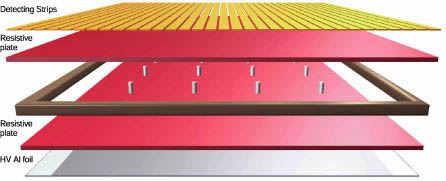
\includegraphics[width=0.50\textwidth]{figures/RPClayers.jpg}
% \caption{}
% \label{fig:RPClayers}
% \end{figure}

% Resistive Plate Chambers (RPCs) are fast gaseous detectors that provide a muon trigger system, consisting of two parallel plates acting as an anode and cathode. The plates are both made of a very high resistivity plastic material and separated by a thin gas volume.

% \begin{itemize}
% 	\item \textbf{Location:} RPCs are deployed in both the barrel ($|\eta| < 1.6$) and endcap ($1.6 < |\eta| < 2.4$) regions.
% 	\item \textbf{Structure:} RPCs are made of resistive plates separated by a gas-filled gap. Typical gas mixtures include tetrafluoroethane (C$_2$H$_2$F$_4$) and sulfur hexafluoride (SF$_6$).
% 	\item \textbf{Working Principle:} Charged particles ionize the gas, creating avalanches that induce a fast signal across resistive plates.
% 	\item \textbf{Time Resolution:} Approximately $1\,\mathrm{ns}$.
% 	\item \textbf{Role:} RPCs provide fast timing information and are primarily used for triggering.
% \end{itemize}

\subsubsection{Gas Electron Multipliers}

Gas Electron Multipliers (GEMs) represent a recent enhancement to the CMS muon detection system. They have been introduced to complement the existing detectors in the forward region near the beampipe, an area subject to increasingly high radiation doses and event rates during Phase-2 of the LHC. Their incorporation aims to improve tracking resolution and trigger performance in this challenging environment.  

Similar to other CMS muon subsystems, GEMs are gaseous detectors. Their distinguishing feature is the GEM foil, a thin ($50\,\mu\mathrm{m}$) insulating polyimide layer coated on both sides with copper conductors. This foil is perforated with microscopic holes arranged in a regular hexagonal pattern. The CMS GEM chambers are structured with two printed circuit boards (PCBs) enclosing a gas volume, within which a stack of three GEM foils is positioned.  

The operational principle of GEMs relies on the ionization of an argon-carbon dioxide (Ar/CO$_2$) gas mixture by incoming charged particles. A strong potential difference applied across the GEM foils generates intense electric fields within the microscopic holes. Electrons liberated during the ionization process drift toward the foils and undergo successive amplification within the holes, producing an electron avalanche. The resulting charge multiplication induces a readout signal on finely spaced readout strips, enabling precise spatial resolution and robust tracking capabilities.  

By integrating GEMs into the CMS muon system, the experiment enhances its ability to detect and reconstruct muons in the high-occupancy forward region, thereby contributing to improved efficiency and performance in the demanding conditions of LHC Phase-2~\cite{CMS:GEMTDR}.  


% \begin{figure}
% \centering
% 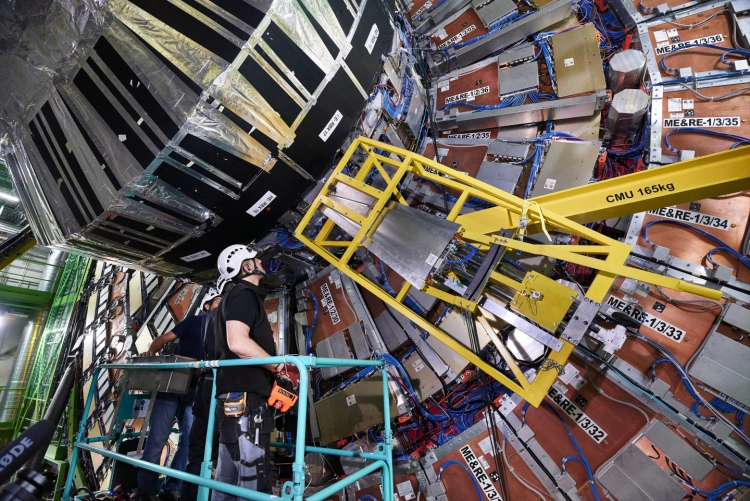
\includegraphics[width=0.80\textwidth]{figures/GEMinstallation.jpg}
% \caption{Gas Electron Multiplier chamber installation.}
% \label{fig:GEMinstallation}
% \end{figure}

% Gas electron multipliers (GEMs) are a new addition to the CMS muon system. They complement existing detectors in the forward regions close to the beampipe, where large radiation doses and high event rates will increase during Phase-2 of the LHC.

% Like the other CMS muon subsystems, GEMs are gaseous detectors. Their key feature is the GEM foil, which consists of a 50 micrometer-thick insulating polymer (polyimide) surrounded on the top and bottom with copper conductors. Throughout the foil, microscopic holes are etched in a regular hexagonal pattern. The CMS GEM chambers consist of two PCBs, containing the gas volume, and a stack of three GEM foils in between. The chambers are filled with an Ar/CO2 gas mixture, which is ionized by incident ionizing particles. A potential difference applied across the foils generates sharp electric fields in the holes. The electrons created during the ionisation process drift towards the foils and are multiplied in the holes. The resulting electron avalanche induces a readout signal on the finely spaced strips.

\section{Triggers and Data Acquisition System}

At the LHC design luminosity, the proton-proton (pp) collision rate exceeds $1\,\mathrm{GHz}$, but only a small fraction of these events are relevant to CMS physics research. Due to storage and computational constraints, only a limited subset can be retained for offline analysis. Efficient event reconstruction is crucial for identifying key physics objects, such as muons, electrons, and jets, within the most significant events.

Muon detection is central to the CMS trigger system, as high-energy muons often signal rare processes, including potential BSM physics. With a bunch crossing rate of $40\,\mathrm{MHz}$, the LHC generates approximately $10^9$ pp interactions per second. Given that each recorded event averages $1.5\,\mathrm{MB}$ and only $\mathcal{O}(1000)$ events per second can be stored, the trigger system must achieve an event rejection factor of $\mathcal{O}(10^6)$ while maintaining high efficiency for key signals.

The CMS trigger system reduces the event rate in real time while preserving sensitivity to rare physics processes. It consists of two stages: the Level-1 (L1) trigger, implemented in custom hardware, and the High-Level Trigger (HLT), which runs software algorithms on a computing farm. Together, these systems ensure that only the most relevant events are stored for analysis~\cite{Cittolin:578006}.

\subsection{Level-1 Trigger}

The L1 trigger rapidly processes detector signals to identify candidate physics objects, such as electromagnetic energy deposits, hadronic jets, and ionization patterns from muons. To manage the $100\,\mathrm{kHz}$ output limit of CMS readout electronics, the trigger dynamically adjusts selection thresholds based on the LHC's instantaneous luminosity.

Using coarse-grained detector data, the L1 trigger selects events with high transverse momentum particles and anomalous energy deposits. Muon chambers---including Drift Tubes (DT), Cathode Strip Chambers (CSC), and Resistive Plate Chambers (RPC)---provide initial $p_T$ estimates for candidate muons. Operating within a strict latency of a few microseconds, the L1 trigger ensures rapid event selection in the LHC’s high-rate environment. The LHC delivers bunch crossings at 40 MHz, and the L1 trigger reduces the incoming event rate to $\sim100\,\mathrm{kHz}$.

\subsection{High-Level Trigger}

The High-Level Trigger (HLT) refines L1 selections by incorporating full-granularity detector data and advanced reconstruction algorithms. For muon identification, it integrates muon chamber signals with precise silicon tracker measurements, improving momentum resolution and suppressing background. By applying more stringent selection criteria, the HLT ensures that only the most promising events are retained for physics analyses.

Events passing the L1 trigger are transferred to front-end readout buffers before being processed by the HLT on a dedicated computing farm. The HLT software further reduces the event rate from $100\,\mathrm{kHz}$ to $1\,\mathrm{kHz}$ for mass storage. Event selection follows a staged approach: initial decisions rely on calorimeter and muon system data, followed by inner tracker pixel information, and ultimately, full event reconstruction when necessary.

To optimize storage efficiency, events are categorized into non-exclusive data streams based on HLT decisions. Most data undergo immediate processing, while lower-priority datasets can be deferred using a technique known as ``parking.'' This capability allows CMS to record additional data on tape at the expense of increased processing latency.

\section{Computing}

Even with the triggers reducing the amount of unnecessary data coming out of our detector, CMS still produces a huge amount of data that must be analyzed---more than 5 petabytes (Pb) per year when running at peak performance. The storage and computational demands of processing such data far exceed the capabilities of a single facility, necessitating a globally distributed computing infrastructure.

To manage and process CMS data efficiently, the Worldwide LHC Computing Grid (WLCG) provides a hierarchical computing architecture, integrating resources from 170 computing centers across 42 countries. This infrastructure consists of four distinct tiers, each with specialized functions~\cite{Cittolin:578006, SHIERS2007219, Bayatyan:838359}.

Following event selection by the trigger system, accepted events are transferred to the CMS Storage Manager for archival storage and subsequent processing. Initially, data are stored on local disks before being transmitted to the Tier-0 center at CERN. This facility is responsible for the initial reconstruction of raw collision data (the first step toward physics analysis) and creates a primary backup before distributing the data to Tier-1 centers for further processing.

Tier-1 centers, located in thirteen national laboratories and research institutes across France, Germany, Russia, Italy, Spain, Taiwan, the United Kingdom, and the United States, receive data from Tier-0. These centers perform a second round of event reconstruction, incorporating refined calibration constants derived from ongoing experimental analysis. They also provide long-term storage and distribute datasets to Tier-2 centers.

Around 160 Tier-2 centers, primarily based at universities and research institutions, receive subsets of data from Tier-1. These facilities are dedicated to specific analyses and large-scale Monte Carlo simulations required for physics studies.

Tier-3 consists of smaller computing clusters, including individual research group resources, which provide additional flexibility for end-user analysis. Unlike the other tiers, Tier-3 centers do not have a formal commitment to WLCG but are crucial for local data processing.

% By leveraging the hierarchical structure of the WLCG, CMS ensures efficient data distribution, storage, and processing, enabling timely analysis of LHC collision events while accommodating the evolving needs of the physics program.


% Even with the triggers reducing the amount of unnecessary data coming out of our detector, CMS still produces a huge amount of data that must be analysed -- more than 5 Pb per year when running at peak performance.

% The ``Tier 0'' center at CERN is the first to reconstruct full collision events, where analysts begin searching for patterns in the data. 
% Then, after CERN creates a primary backup, the data is sent to large ``Tier 1'' computer centers located in seven different countries: France, Germany, Italy, Spain, Taiwan, the UK, and the US. 
% At these centers, the events are reconstructed again, with improved calculations using refined calibration constants based on experimental information.

% Tier 1 centers begin to interpret and analyze the particle events, compiling the results to identify emerging patterns. Simultaneously, each Tier 1 center sends the most complex events to a network of around 40 ``Tier 2'' facilities for further specialized analysis. This tiered system efficienty processes all CMS data while also allowing information to be distributed globally, regularly updated by the LHC Computing Grid.

\section{Particle Reconstruction}

The Particle Flow (PF) algorithm is designed to achieve a comprehensive reconstruction and identification of all stable particles in an event by leveraging information from all CMS sub-detectors. By optimally combining measurements from the tracker, calorimeters, and muon systems, the PF algorithm determines the direction, energy, and particle type with high precision. I will introduce the concept here, but elaborate on the details of particle reconstruction and selection as they apply to this thesis in Section~\ref{sec:recoandsel}.

The reconstructed list of individual particles serves as the foundation for higher-level physics objects. It is treated similarly to final-state particles generated by Monte Carlo event generators, enabling the construction of hadronic jets, from which the kinematic properties of originating quarks and gluons can be inferred. Additionally, the PF algorithm plays a crucial role in determining missing transverse energy (MET), providing an estimate of the momentum carried away by neutrinos and other undetected particles. Furthermore, it facilitates the reconstruction and identification of particles through their decay products, enhancing the sensitivity of CMS analyses to a wide range of physics processes~\cite{Beaudette:1645993}.

% The Particle Flow (PF) algorithm aims at reconstructing and identifying all stable particles in the event with a thorough combination of all CMS sub-detectors towards an optimal determination of their direction, energy and type. This list of individual particles is then used, as if it came from a Monte-Carlo event generator, to build jets (from which the quark and gluon energies and directions are inferred), to determine the missing transverse energy (which gives an estimate of the direction and energy of the neutrinos and other invisible particles), to reconstruct and identify particles from their decay products, and more \cite{Beaudette:1645993}.

\section{Alignment of the CMS Tracker}

As aforementioned, the precision of the silicon tracker is critical to CMS, especially in measuring the trajectories of particles within our solenoid. The alignment of the tracker was also crucial to our research group, which contributes to the experimental service effort and is the sole maintainer of one of primary tracker alignment algorithms. Over the course of my thesis, I ran alignment campaigns and validated alignment candidates, as well as provided some updates to our Hits-and-Impact-Points alignment algorithm also known as ``HipPy''---the algorithm and my efforts are described in Sections~\ref{sec:alignalgo}~and~\ref{sec:alignment}, respectively.

\subsection{Parameterization}

Various parts of the CMS detector have been detailed in Section~\ref{chap:chap-3.2-CMS}. The pixel detector and strip tracker, in particular, can be further divided into their subdetector structures or modules. The hierarchical structure of the CMS tracker is illustrated in Figure~\ref{fig:HLS}. 

\begin{figure}[!hbt]
    \begin{center}
        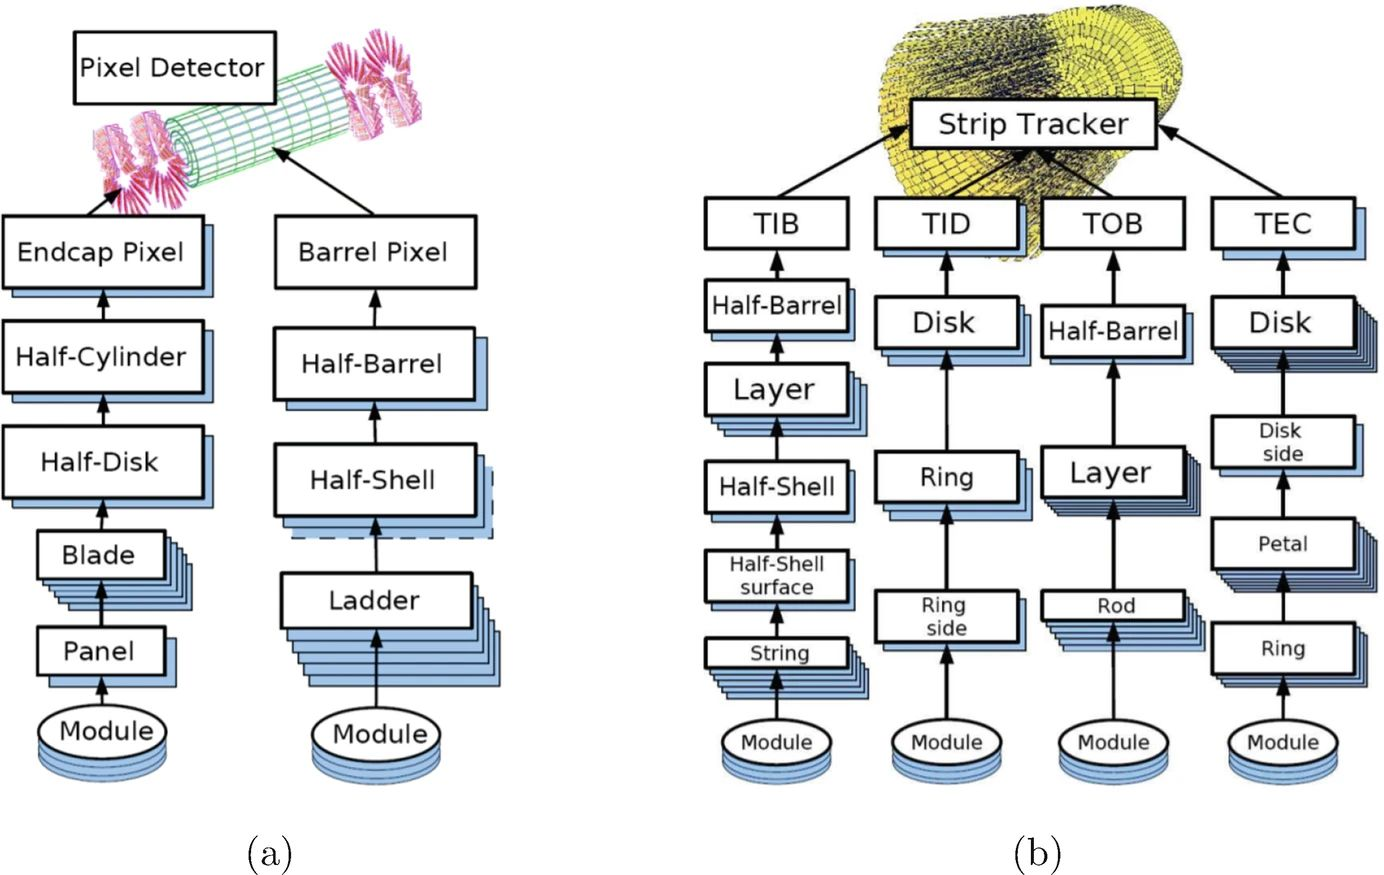
\includegraphics[width=0.8\textwidth,clip] {HLS.jpg}
        \caption{Hierarchical structures of the pixel detector and strip tracker \cite{WAdam_2009}.}
        \label{fig:HLS}
    \end{center}
\end{figure}

The accuracy of track reconstruction is significantly affected by uncertainties in module positioning. If the module position is not precisely known, the recorded hit positions and the expected impact points (extrapolated from other measured hits) of a track will exhibit systematic displacements. The discrepancy between these two quantities, expressed in the local coordinate system of the module, defines the \emph{track-hit residuals} illustrated in Figure~\ref{fig:overlapHits}~\cite{Karimaki:926537}.  

\begin{figure}[!hbt]
    \begin{center}
        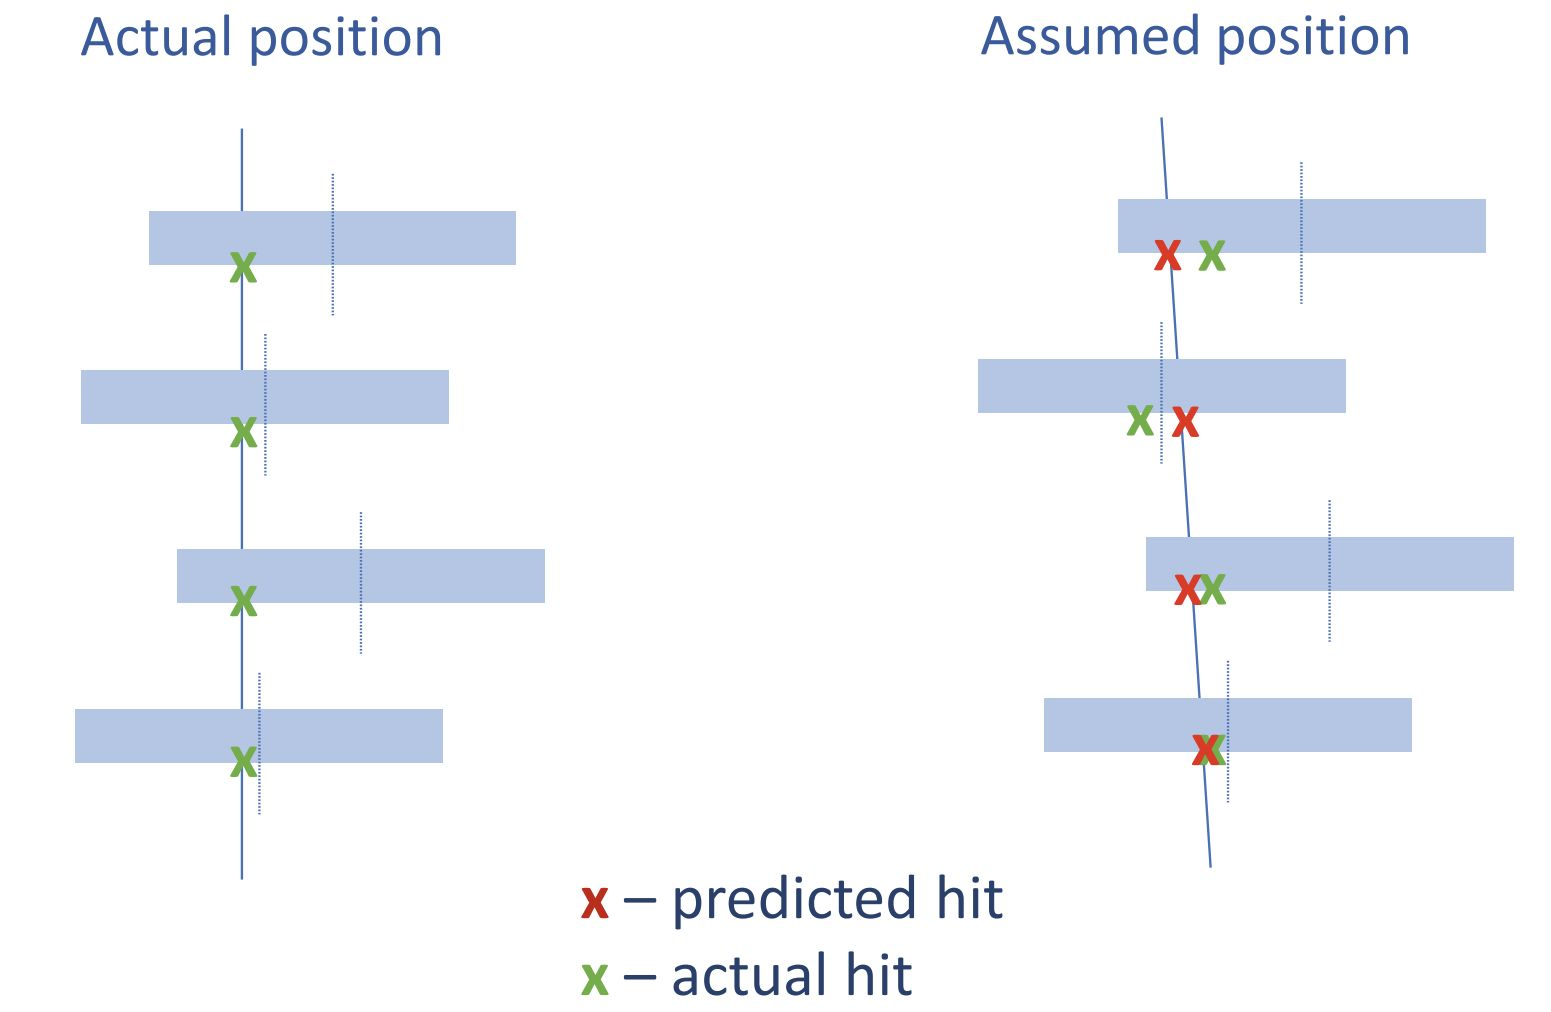
\includegraphics[width=0.7\textwidth,clip] {overlapHits.jpg}
        \caption{Simple illustration of a track through misaligned layers \cite{2022166795}.}
        \label{fig:overlapHits}
    \end{center}
\end{figure}

Each detector module is parameterized within a local coordinate system $(u, v, w)$, as illustrated in Figure~\ref{fig:TrackerParam}. The coordinate axes are defined such that the $w$-axis is normal to the module plane, while the $u$- and $v$-axes lie within the plane. The $u$-axis is oriented along the more sensitive measurement direction. Rotational misalignments of the module are described by three angles: $\alpha$, $\beta$, and $\gamma$, which correspond to rotations about the $u$-, $v$-, and $w$-axes, respectively. Precise calibration of these parameters is essential for minimizing systematic biases in track reconstruction ~\cite{Karimaki:926537, Karimaki:2003bd}.

\begin{figure}[!hbt]
    \begin{center}
        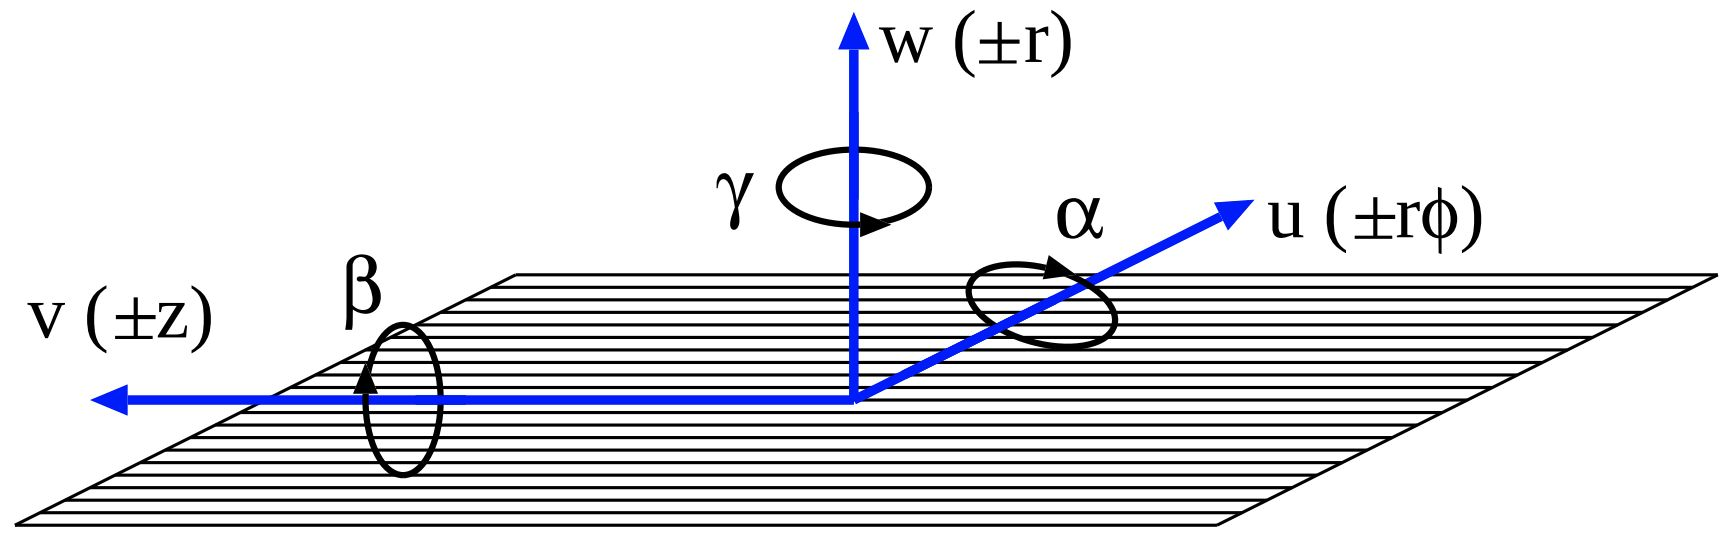
\includegraphics[width=0.8\textwidth,clip] {TrackerParam.jpg}
        \caption{Example local coordinates of a module. Global parameters are shown in parentheses for modules in the TIB and TOB \cite{WAdam_2009}.}
        \label{fig:TrackerParam}
    \end{center}
\end{figure}

Each module is also parameterized in a global coordinate system $(x, y, z)$. The transformation from the global coordinate system to the local module coordinate system is expressed as
\begin{equation}
    \mathbf{q} = \mathbf{R} (\mathbf{r} - \mathbf{r_0}),
\end{equation}  
where $\mathbf{r} = (x,y,z)$ represents the position in the global coordinate system, $\mathbf{q} = (u,v,w)$ denotes the corresponding position in the local module system, $\mathbf{r_0} = (x_0,y_0,z_0)$ is the position of the detector module center in global coordinates, and $\mathbf{R}$ is a rotation matrix that accounts for the module's orientation. This transformation ensures that local hit positions can be consistently related to the global detector geometry. 

Due to the hierarchal nature of our modules, it is sometimes useful to describe the position of a group of sensors belonging to a composite tracker structure. In this case, we use a simple change of variable to represent the same definitions as above, but for the larger structures. $\mathbf{g}$ represents the coordinates in the composite basis, $\mathbf{g_0}$ gives the composite origin in global coordinates, and $\mathbf{G}$ rotates from the global to the composite system~\cite{Karimaki:926537}.

Initially, the rotation matrix $\mathbf{R}$ and the detector positions $\mathbf{r_0}$ can be determined through detector assembly and survey measurements. Then, after assembly, these parameters will be corrected incrementally through alignment procedures to account for mechanical shifts, thermal expansion, and other systematic effects that may alter the module positions over time. It should be noted that tracker alignment is not a physical procedure, but rather a correction of our interpretation of the detector data in software. 
% Accurate alignment is essential to minimize track-hit residuals and ensure precise reconstruction of particle trajectories.



% Hit positions and impact points of a track are systematically displaced if the module position is not known correctly.

% The difference in local module coordinates between these two quantities are the ``track-hit residuals'' \cite{Karimaki:926537}.

% Modules are parameterized as seen in Fig.~\ref{fig:TrackerParam}:
% \begin{itemize}
%     \item w axis is normal to the module
%     \item u and v axes are in the plane
%     \item u axis more sensitive to direction of measurement
%     \item Angles $\alpha$, $\beta$, and $\gamma$ describe rotations around u, v, w respectively
% \end{itemize}

% Various parts of the CMS detector have been detailed in Section~\ref{chap:chap-3.2-CMS}. The pixel detector and strip
% tracker, in particular, can be further divided into their subdetector structures or modules. The hierarchical structure of the CMS tracker is illustrated in Figure~\ref{fig:HLS}. 

% Hierarchical systems:
% \begin{itemize}
%     \item \{r, g, q\} = coordinates in \{global, composite, local\} system
%     \item \{R, G\} = rotations between global and \{local, composite\} system
% \end{itemize}



\subsection{Algorithms}\label{sec:alignalgo}

Two primary algorithms are used by CMS to minimize track-hit residuals and improve alignment: Millepede and HipPy. 

\subsubsection{Millepede}

Millepede-II (colloquially referred to as ``Millepede'' or ``MP'') employs a global matrix approach, eliminating the need for iterative procedures. Millepede-II~\cite{BLOBEL20065} is an upgraded version of the original Millepede~\cite{blobel2002newmethodhighprecisionalignment} program, designed to perform a global fit by minimizing the $\chi^2$ function while simultaneously accounting for both track and alignment parameters. Since angular corrections remain small, the problem can be effectively linearized while remaining a suitable approximation for alignment studies.

The optimization MP performs is structured to focus exclusively on the $n$ alignment parameters, reducing the problem to solving a matrix equation of size $n$~\cite{WAdam_2009}. The $\chi^2$ function, expressed in terms of both local track parameters $\mathbf{q}$ and global alignment parameters $\mathbf{p}$, is given by  
\begin{equation}
\chi^2(\mathbf{p},\mathbf{q}) = \sum_{j} \sum_{i} \frac{\left(y_{ji} - f_{ji}(\mathbf{p}, \mathbf{q_j})\right)^2}{\sigma^2_{ji}}
\end{equation}

where $y_{ji}$ represents uncorrelated hit measurements of track $j$ with associated uncertainties $\sigma_{ji}$, while $f_{ji}(\mathbf{p}, \mathbf{q_j})$ denotes the predicted measurement based on the alignment and track parameters. Given reasonable initial estimates $\mathbf{p_0}$ and $\mathbf{q_j}_0$, the function $f_{ji}$ can be linearized. Applying the least-squares method to minimize $\chi^2$ results in a system of linear equations, with one equation per alignment parameter and all the track parameters of each track~\cite{WAdam_2009}.

The system of equations can be reduced, ultimately leading to a matrix equation of the form $\mathbf{C} \mathbf{a} = \mathbf{b}$ where $\mathbf{a}$ corresponds to small corrections to the initial alignment parameters $\mathbf{p_0}$. This formulation allows for efficient computation, making Millepede-II particularly well-suited for large-scale alignment tasks.

% \begin{equation}
% \mathbf{C} \mathbf{a} = \mathbf{b}
% \end{equation}



% \begin{figure}[!hbt]
%     \begin{center}
%         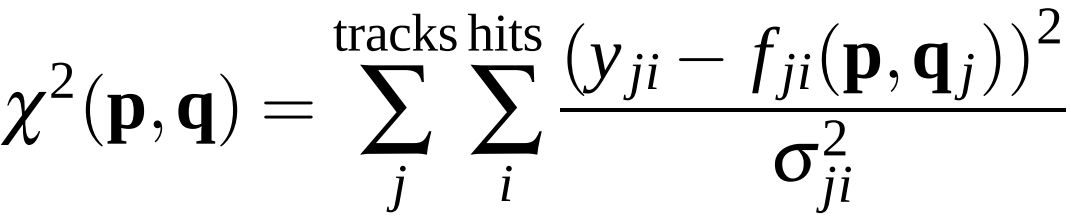
\includegraphics[width=0.8\textwidth,clip] {chi2MPiteration.jpg}
%         \caption{$\Xi^2$ function for MILLEPEDE-II global fit \cite{WAdam_2009}.}
%         \label{fig:chi2MPiteration}
%     \end{center}
% \end{figure}

% \begin{equation}
% \label{eq:MPX2}
% \begin{gathered}
% \mathcal{X} ^2 (p, q) = \Sigma_j^{tracks} \Sigma_i^{hits} \frac{(y_{ji} - f_{ji}(p, q_j))^2}{\sigma_{ji}^2}
% \end{gathered}
% \end{equation}

% Unlike HipPy, MILLEPEDE-II (MP) opts to use a global matrix and forgoes the iterative approach.

\subsubsection{HipPy}

The Hits-and-Impact-Points (HIP) algorithm~\cite{Karimaki:2003bd, Karimaki:926537} served as the predecessor to what later became HipPy. Initially implemented during the commissioning of the CMS tracker~\cite{WAdam_2009} and extensively used throughout Run 1~\cite{CMSCollaboration_2010, Chatrchyan:1667597}, the algorithm underwent significant modifications over time~\cite{BROWN2009467}. These refinements led to the development of an improved version, designated as Hits-and-Impact-Points-Past-Year-1 (HipPy), which was formally introduced at the start of Run 2. 

\begin{figure}[!hbt]
    \begin{center}
        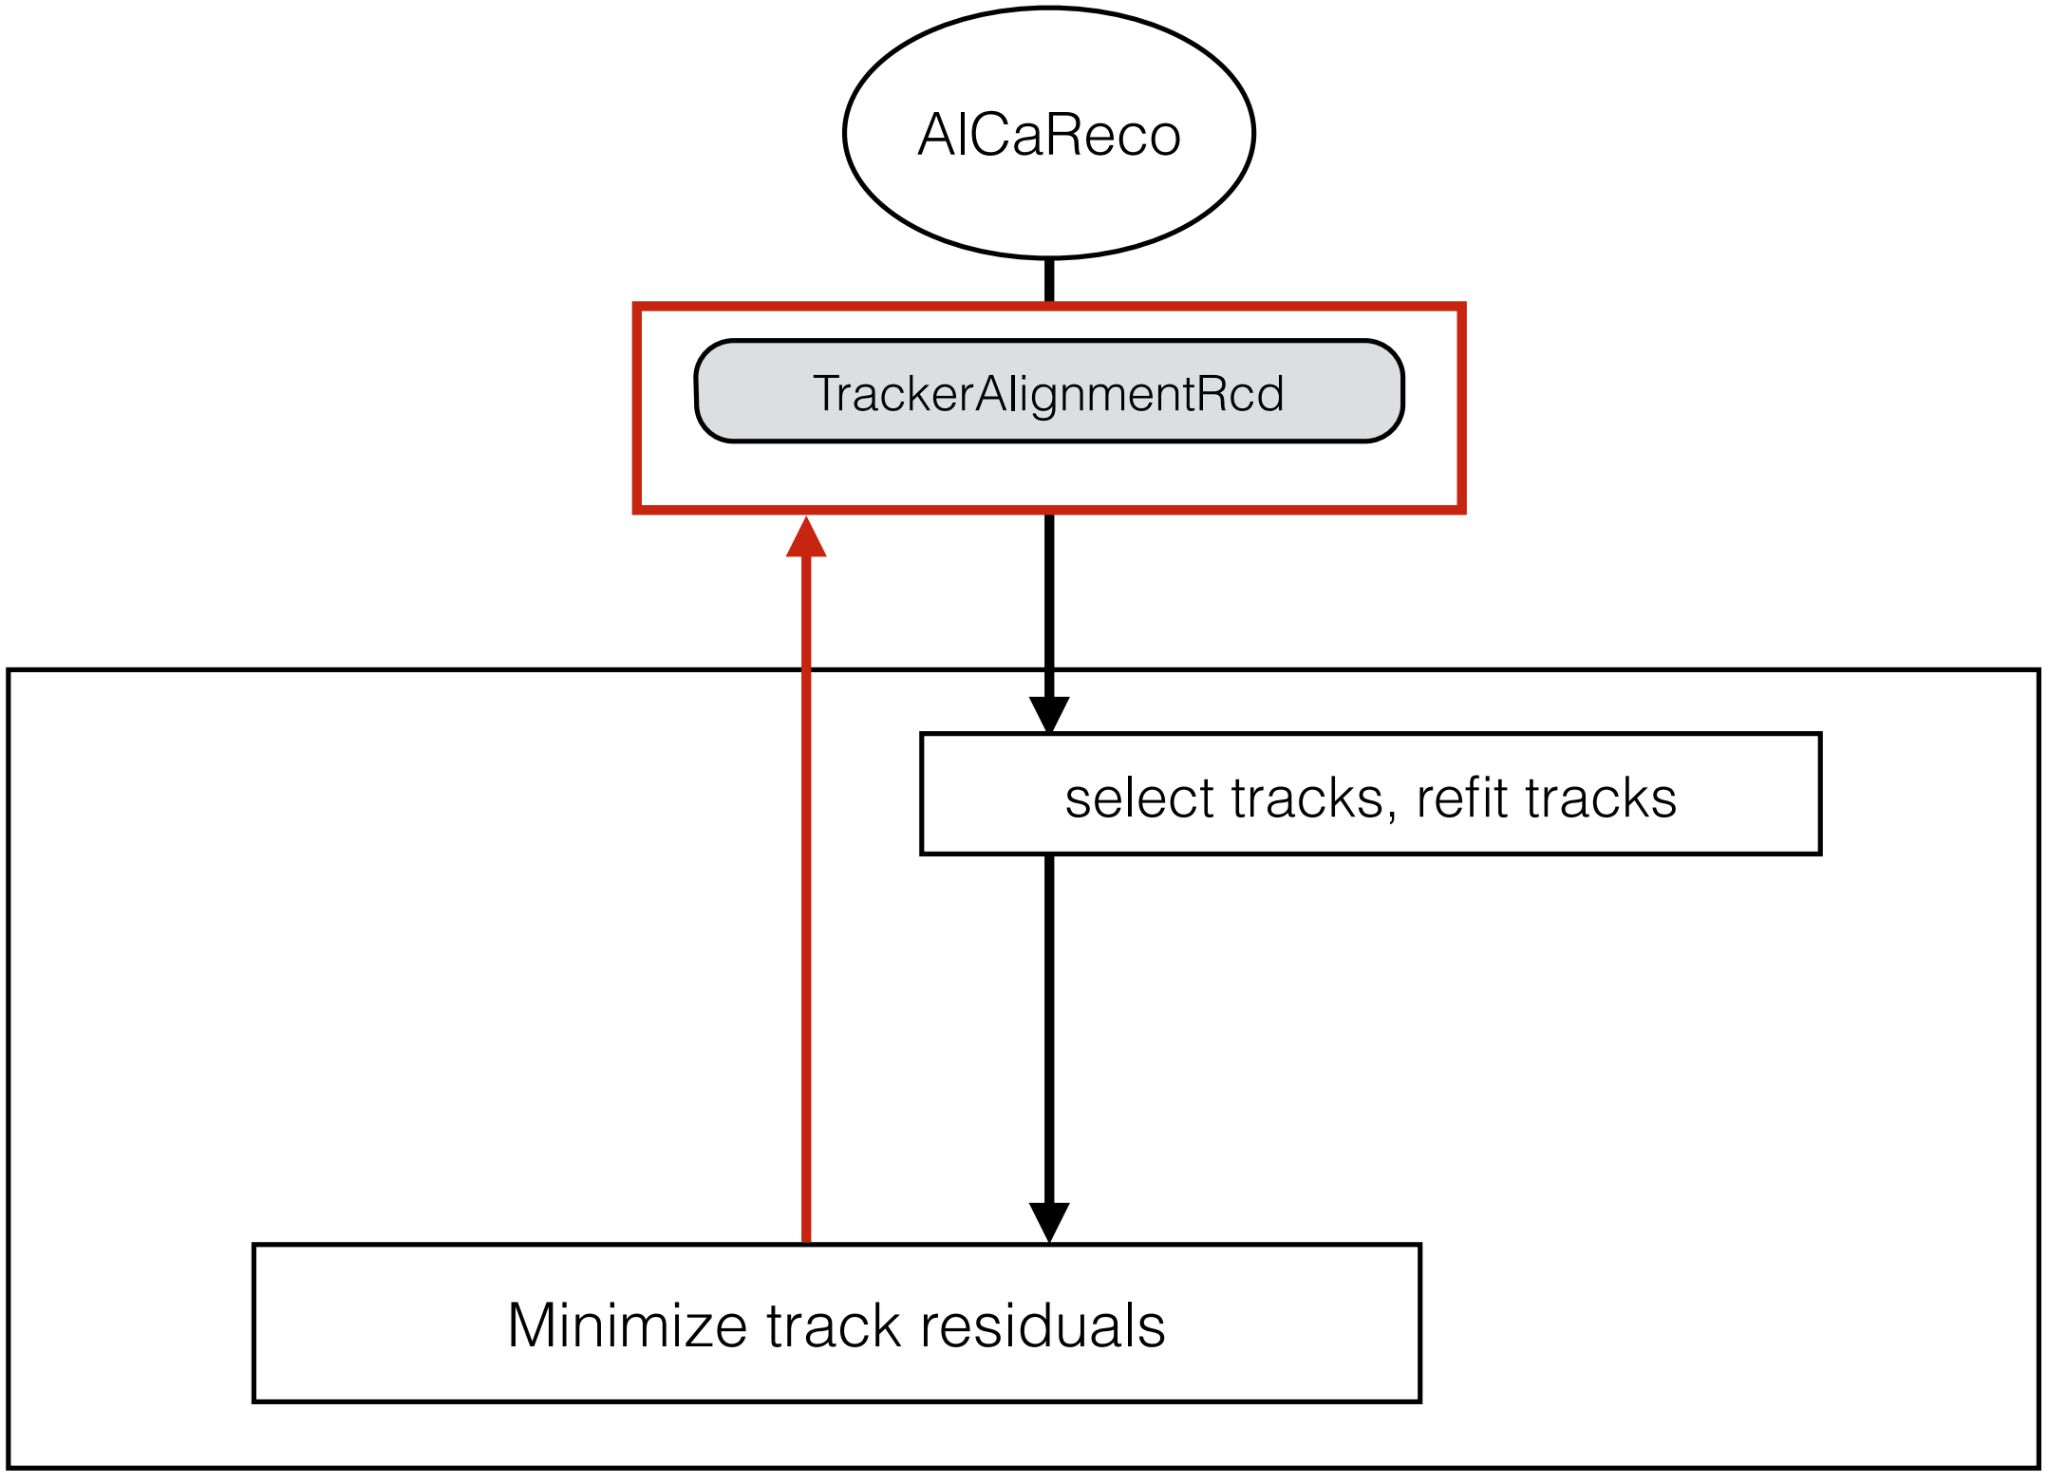
\includegraphics[width=0.8\textwidth,clip] {HIP.jpg}
        \caption{Process diagram of the Hits-and-Impact-Points (HIP) alignment algorithm \cite{2022166795}.}
        \label{fig:HIP}
    \end{center}
\end{figure}

Key advancements in the alignment methodology after CMS' first year online included the addition of three alignment parameters to account for sensor curvature, extending beyond the conventional six parameters that describe sensor position and orientation. Enhancements were also made to allow for the weighting of specific input types, the introduction of a sequential and hierarchical alignment strategy across multiple time periods (multi-IOV), and the incorporation of optional mass and vertex constraints in events with well-characterized underlying physics processes. These improvements significantly enhanced the alignment precision and stability, contributing to the success of Run 2. The HipPy-based alignment parameters were adopted for CMS data reconstruction and were used in both prompt and end-of-year (EOY) alignments alongside Millepede-II (MP) constants~\cite{BROWN2009467}. 

\begin{figure}[!hbt]
    \begin{center}
        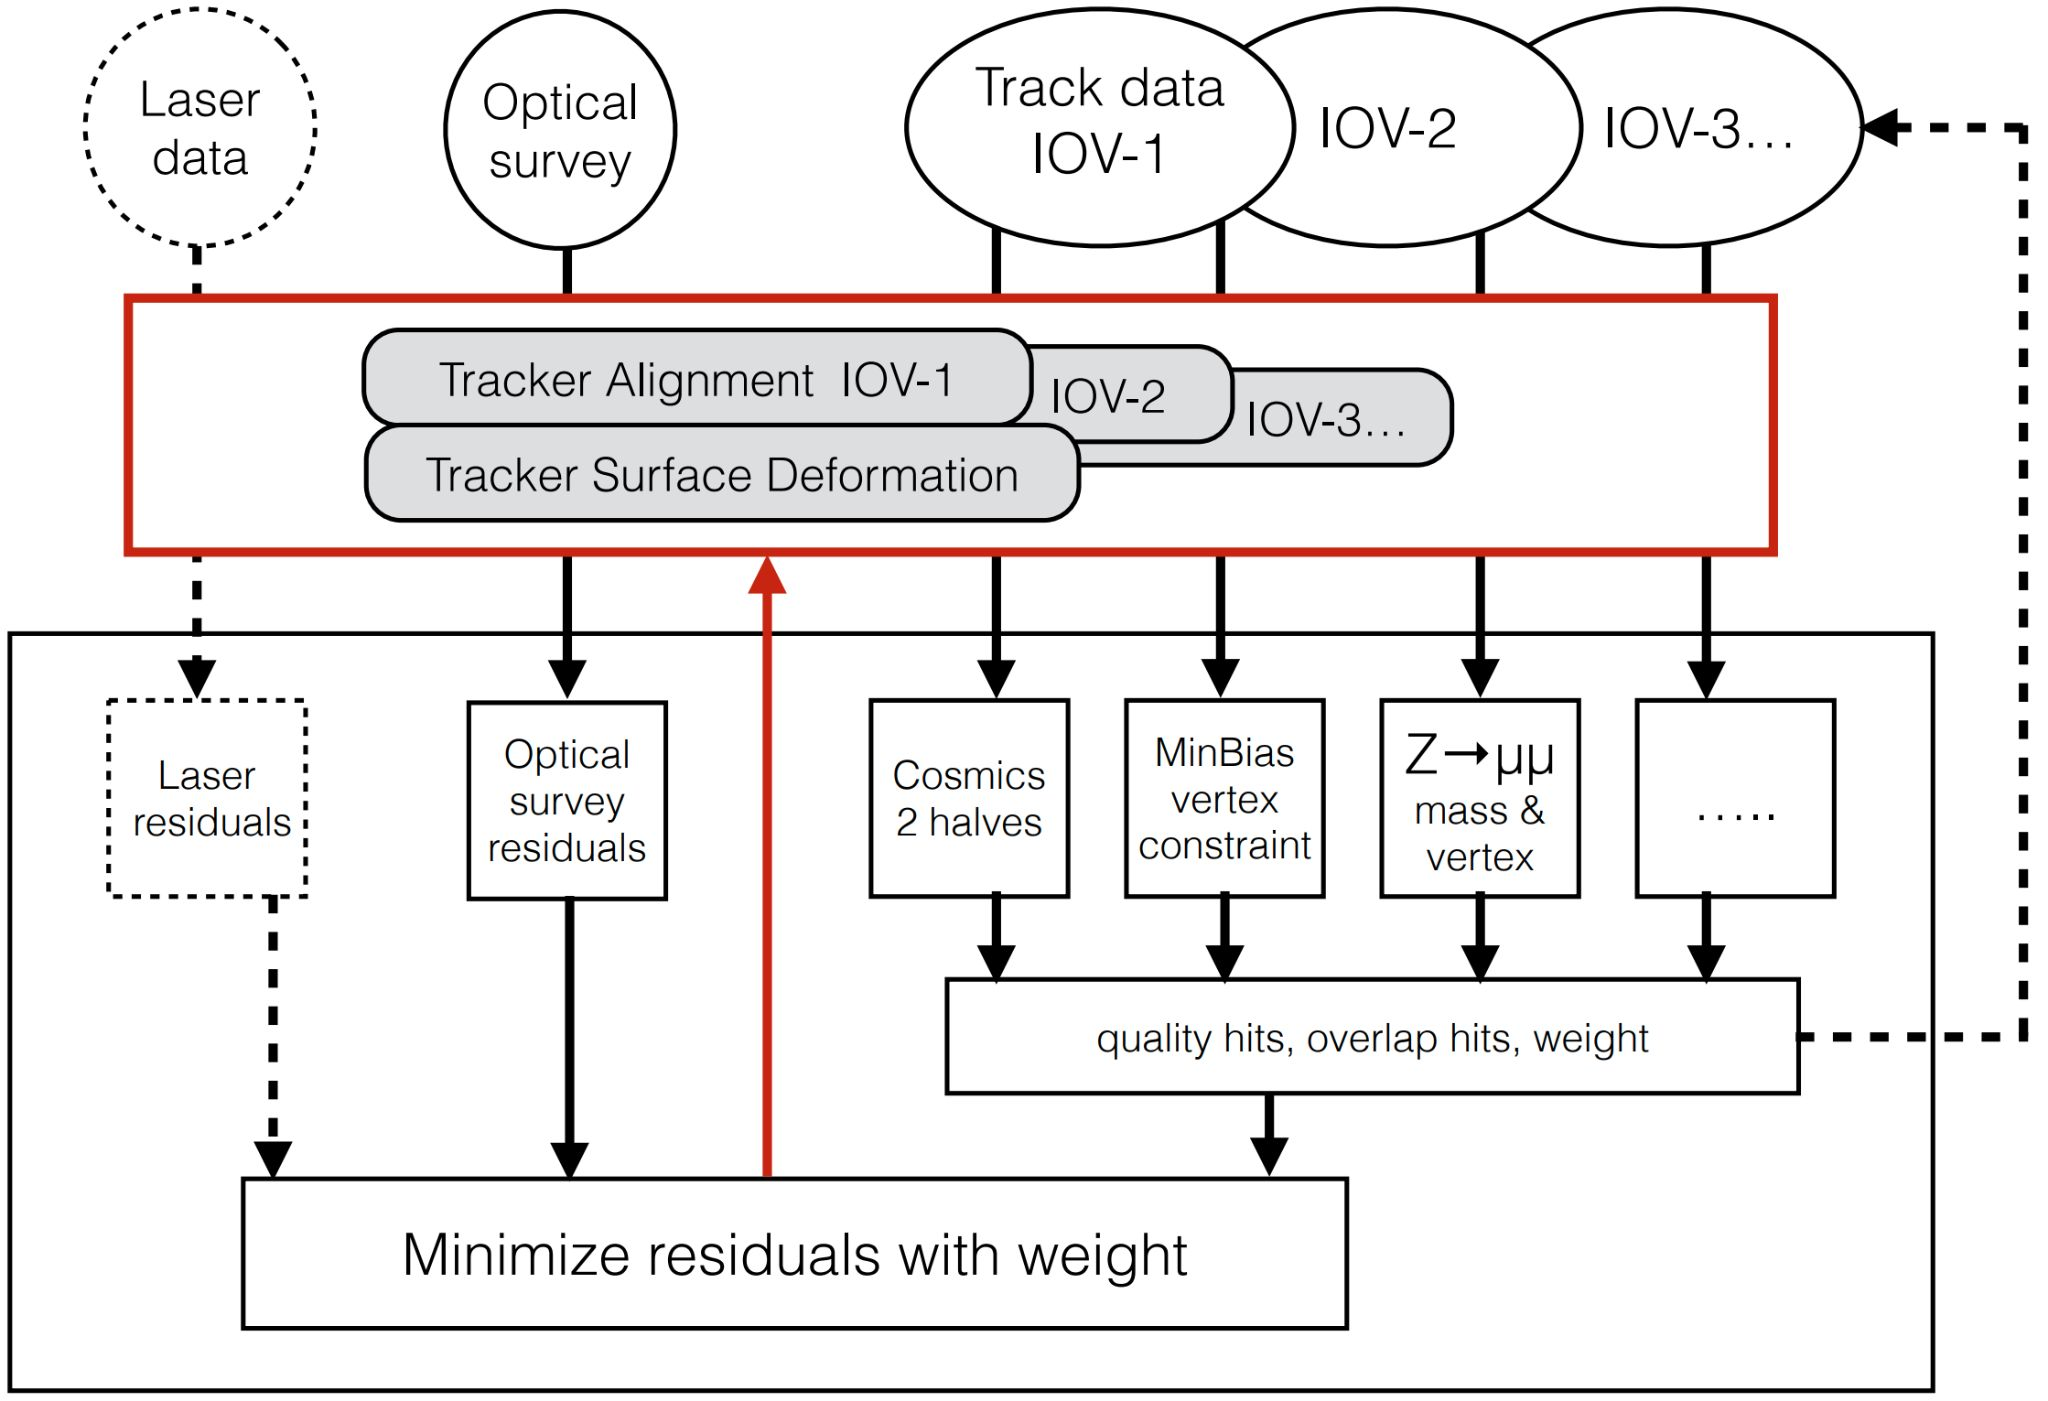
\includegraphics[width=0.8\textwidth,clip] {HipPy.jpg}
        \caption{Process diagram of the Hits-and-Impact-Points-Past-Year-1 (HipPy) alignment algorithm~\cite{2022166795}.}
        \label{fig:HipPy}
    \end{center}
\end{figure}

The fundamental principle of HipPy involves iteratively refining the local alignment of individual detector sensors while keeping all other parameters fixed. The procedure begins with loading track data and hit measurements, followed by track fitting using the current estimate of alignment parameters. A \(\chi^2\) function, defined in Eq.~\eqref{eq:HIPX2}, is computed for the selected hits for a given sensor (module). For each sensor, the alignment parameters are updated by minimizing \(\chi^2\) with respect to local shifts while holding all other sensor parameters constant. The process iterates until convergence is achieved.

% \begin{equation}
% \label{eq:HIPX2}
% \mathcal{X}^2 = \sum_{i}^{\text{hits}} \epsilon_i^T(p) V_i^{-1} \epsilon_i(p),
% \end{equation}

% where \(\epsilon_i(p)\) represents the residuals as a function of alignment parameters \(p\), and \(V_i\) is the corresponding covariance matrix. 

The \(\chi^2\) function for HipPy can be written using a covariance matrix \(\mathbf{V}\) of the measurement uncertainties

\begin{equation}
\label{eq:HIPX2}
\mathcal{X}^2 = \sum_{i}^{\text{hits}} \mathbf{r}_i^T(\mathbf{p}, \mathbf{q}) \mathbf{V}_i^{-1} \mathbf{r}_i(\mathbf{p}, \mathbf{q})
\end{equation}

where \(\mathbf{r}_i(\mathbf{p}, \mathbf{q})\) are residuals dependent on both track parameters \(\mathbf{q}\) and alignment parameters \(\mathbf{p}\). The update step for alignment parameters is obtained from

\begin{equation}
\label{eq:HPpm}
\mathbf{p}_m = \left[\sum_{i}^{\text{hits}} \mathbf{J}_i^T \mathbf{V}_i^{-1} \mathbf{J}_i\right]^{-1} \left[\sum_{i}^{\text{hits}} \mathbf{J}_i^T \mathbf{V}_i^{-1} \mathbf{r}_i\right]
\end{equation}

where \(\mathbf{J}_i\) denotes the Jacobian matrix of residuals with respect to the alignment parameters, and can be solved analytically via the small angle approximation. Correlations between different modules and effects on the track parameters are accounted for by iterating the minimization process and by refitting the tracks with new alignment constants after each iteration~\cite{WAdam_2009}. 

A key advantage of HipPy is its seamless integration with the CMS software framework, particularly in the context of track reconstruction. This integration enables the use of kinematic constraints such as mass and vertex constraints, which improve alignment precision. Additionally, HipPy simplifies development by leveraging Kalman filter-based algorithms. The algorithm treats the position and orientation of each sensor independently in every iteration. While each step consists of a straightforward matrix inversion~\cite{WAdam_2009, Karimaki:926537}, multiple iterations are required to account for correlations between sensor parameters. This necessitates repeated track fitting which can become time- and CPU-intensive. 

% While multiple iterations are required to account for correlations between sensor parameters—necessitating repeated track fitting—each step consists of a straightforward matrix inversion~\cite{WAdam_2009, Karimaki:926537}.

% \begin{figure}[!hbt]
%     \begin{center}
%         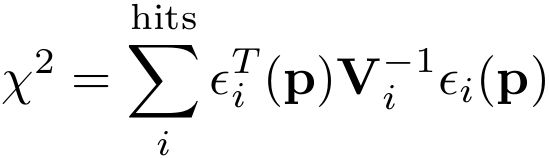
\includegraphics[width=0.8\textwidth,clip] {chi2HPiteration.jpg}
%         \caption{$\Xi^2$ function for HipPy fit.}
%         \label{fig:chi2HPiteration}
%     \end{center}
% \end{figure}

% \begin{figure}[!hbt]
%     \begin{center}
%         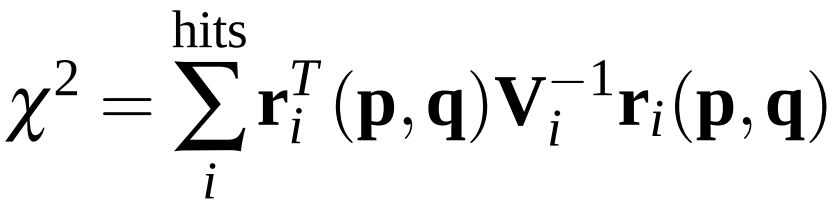
\includegraphics[width=0.8\textwidth,clip] {chi2HPiteration2.jpg}
%         \caption{$\Xi^2$ function for HipPy fit.}
%         \label{fig:chi2HPiteration2}
%     \end{center}
% \end{figure}

% \begin{figure}[!hbt]
%     \begin{center}
%         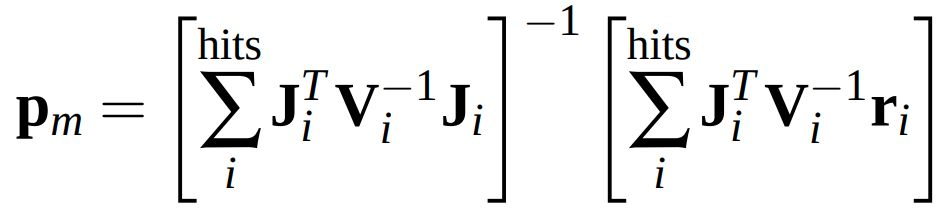
\includegraphics[width=0.8\textwidth,clip] {pmHPiteration.jpg}
%         \caption{Alignment parameters $p_m$ for HipPy fit.}
%         \label{fig:pmHPiteration}
%     \end{center}
% \end{figure}

%The ``hits-and-impact-points'' (HIP) algorithm \cite{Karimaki:2003bd,Karimaki:926537} precedes what we now call HipPy.
% Utilized during commissioning \cite{WAdam_2009} of the CMS tracker and for Run 1 \cite{CMSCollaboration_2010,Chatrchyan:1667597}.

% Several notable features were added over time \cite{BROWN2009467} and the improved algorithm was renamed to “hits-and-impact-points-past-year-1” (HipPy) at the start of Run 2. 

% Improvements to the alignment algorithm since Run 1:
% \begin{itemize}
%     \item The inclusion of 3 alignment parameters to describe sensor curvature (beyond the 6 position/orientation coordinates)
%     \item The ability to weight certain types of input
%     \item The option to perform sequential, hierarchical alignment over multiple time periods (multi-IOV)
%     \item Optional mass and/or vertex constraints in certain types of events with known physics process
% \end{itemize}

% These features proved invaluable during Run 2, with successful HipPy-based alignment constants used in CMS data reconstruction (along with MP objects) in the prompt and EOY alignments\cite{BROWN2009467}.

% The basic outline of the hits-and-impact-points (HIP) algorithm is as follows \cite{BROWN2009467}:
% \begin{itemize}
%     \item Load track data and hits
%     \item The tracks are fit using the current estimate of the alignment parameters
%     \item Hit $\mathcal{X} ^2$ are computed for the selected hits, following the definition in Eq.~\ref{eq:HIPX2}
%     \item Minimize each sensor’s $\mathcal{X} ^2$ w.r.t. a change in only that sensor’s local alignment
%     \item Hold the parameters of every other sensor fixed
%     \item Calculate for every sensor
%     \item Update the alignment parameters for all sensors with the computed change to the original estimate
%     \item Use the updated local alignment to fit the tracks for the next iteration
%     \item Repeat the process until the alignment converges
% \end{itemize}

% \begin{equation}
% \label{eq:HIPX2}
% \begin{gathered}
% \mathcal{X} ^2 = \Sigma_i^{hits} \epsilon_i^T(p) V^{-1}_i \epsilon_i(p)
% \end{gathered}
% \end{equation}

% \begin{itemize}
%     \item HipPy leverages full integration of CMS software, which is helpful especially for track reconstruction
%     \item Can make use of any constraint (e.g. mass, vertex) defined in that software
%     \item Adds flexibility and simplifies development (e.g. Kalman filter)
%     \item Position and orientation of each sensor are determined independently of other sensors in every iteration
%     \item Multiple iterations are required to solve correlations between sensor parameters (requires multiple track fits)
%     \item But each iteration is a straightforward application of a small matrix inversion
% \end{itemize}

% \begin{equation}
% \label{eq:HPX2}
% \begin{gathered}
% \mathcal{X} ^2 = \Sigma_i^{hits} r_i^T(p, q) V^{-1}_i r_i(p, q)
% \end{gathered}
% \end{equation}

% \begin{equation}
% \label{eq:HPpm}
% \begin{gathered}
% p_m = [\Sigma_i^{hits} J^T_i V^{-1}_i J_i]^{-1} [\Sigma_i^{hits} J^T_i V^{-1}_i r_i]
% \end{gathered}
% \end{equation}







% \begin{figure}[!hbt]
%     \begin{center}
%         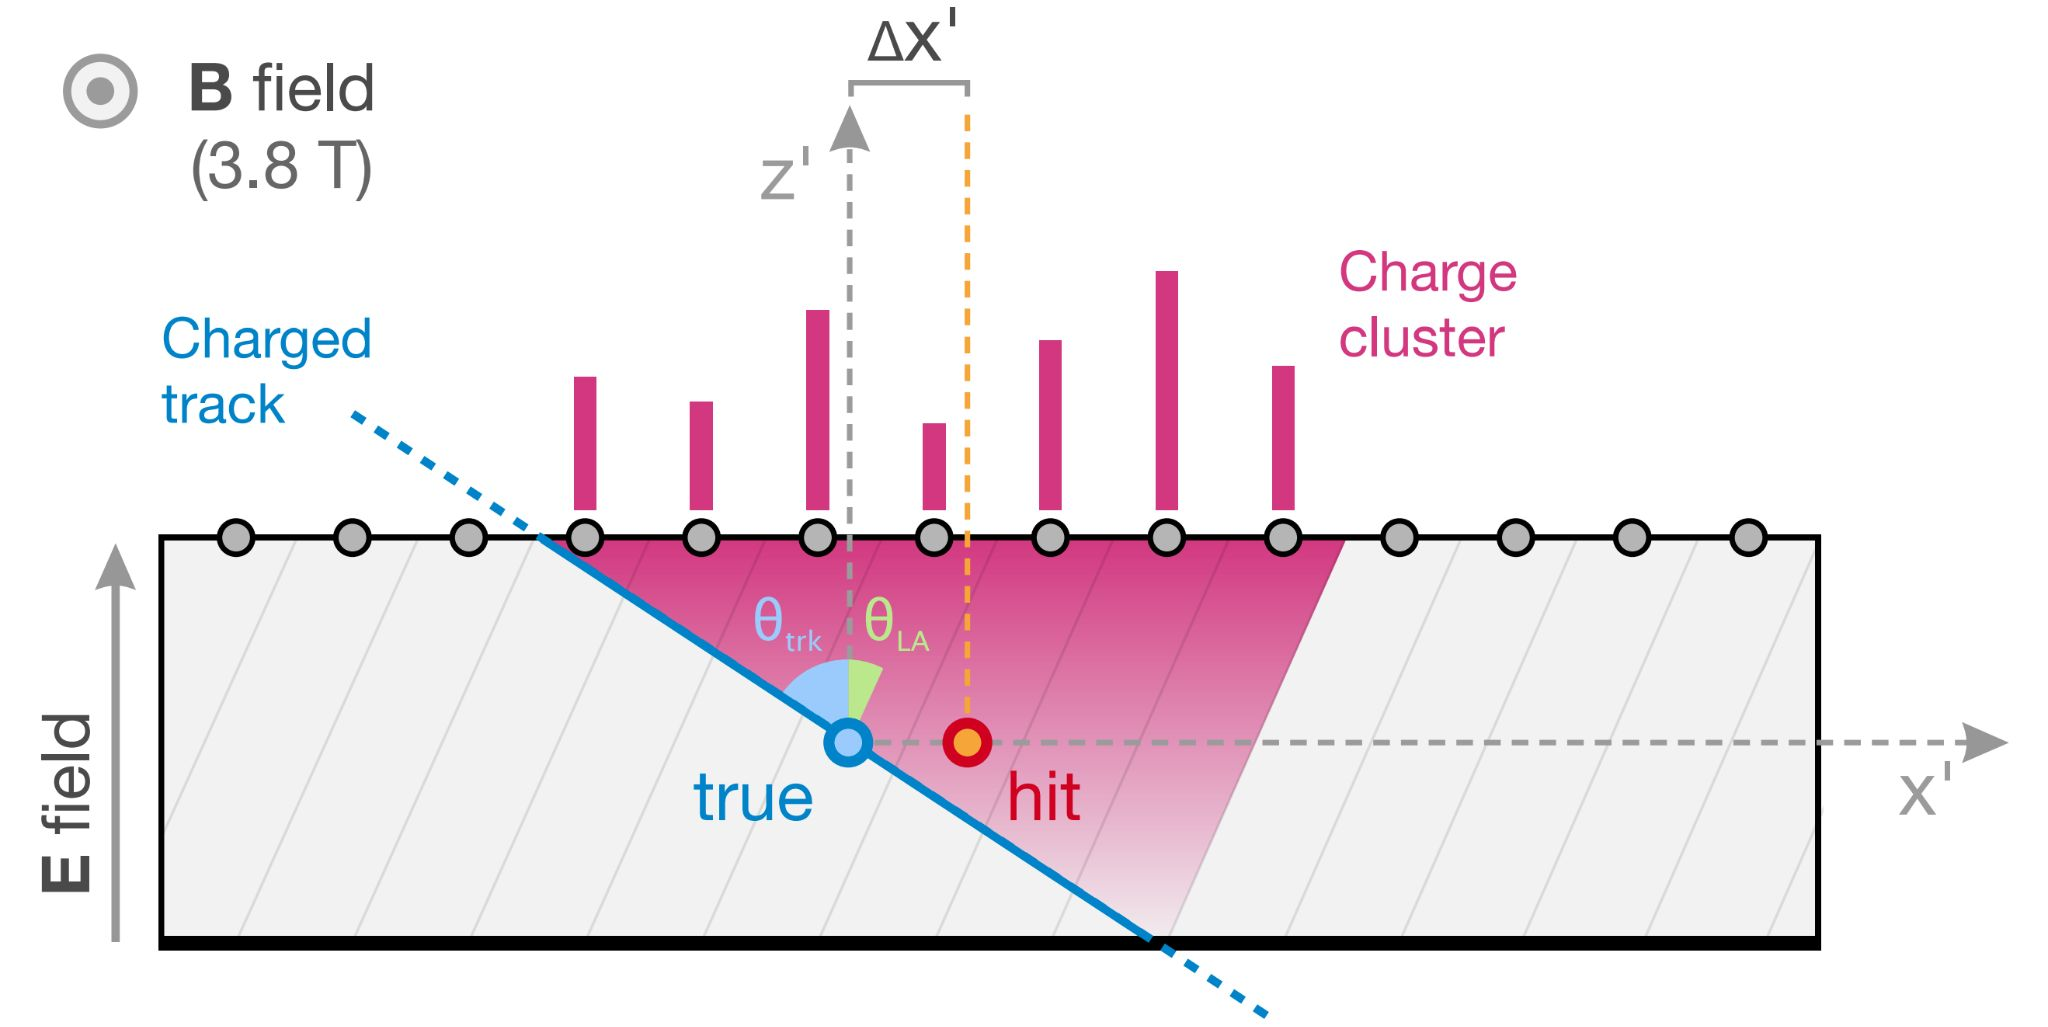
\includegraphics[width=0.8\textwidth,clip] {siliconmodule.jpg}
%         \caption{Transverse view of a silicon module \cite{2022166795}.}
%         \label{fig:siliconmodule}
%     \end{center}
% \end{figure}

\subsection{Validation}

Several validation methods are used within CMS to quantify the quality of calculated alignment parameters. Some common validation methods include geometry comparisons, distribution of the median of residuals, primary vertex, cosmic track splitting, and $Z\to\mu\mu$ or ``dimuon'' validation~\cite{2022166795}.

\subsubsection{Geometry Comparison}

Geometry comparisons provide a direct and effective means of visualizing differences between tracker alignments. Once an alignment fit is performed, the resulting geometry is compared against a reference geometry, which may correspond to the design geometry or a previously aligned dataset. Systematic differences observed in such comparisons can reveal potential distortions in the tracker structure. While geometry comparisons alone do not establish the validity of systematic shifts in module positions, they serve as an essential diagnostic tool, offering insights into possible alignment effects.

Unphysical distortions, identifiable through detector design constraints, can signal biases in the alignment procedure. The geometry comparison framework, adapted from HipPy’s optical survey constraint tools, aligns two geometries by applying translations and rotations before computing their differences. 
% , treating the residuals as survey constraints.  

To facilitate meaningful comparisons, global shifts and rotations of large structures are removed, allowing for precise measurement of module displacements, denoted as \( \Delta z \), \( \Delta r \), and \( \Delta \phi \), as functions of \( z \), \( r \), and \( \phi \), respectively. Additionally, the remaining three spatial coordinates (\( x \), \( y \), and \( z \)) and three angular rotations can also be visualized in a similar manner. Since geometry comparison validation does not rely on reconstructed track data, it can be applied universally with respect to any reference geometry, including design, survey, or previously aligned track-based geometries. An example of such a validation is shown in Figure~\ref{fig:global_tracker_1_final}.

\begin{figure}[!hbt]
    \begin{center}
        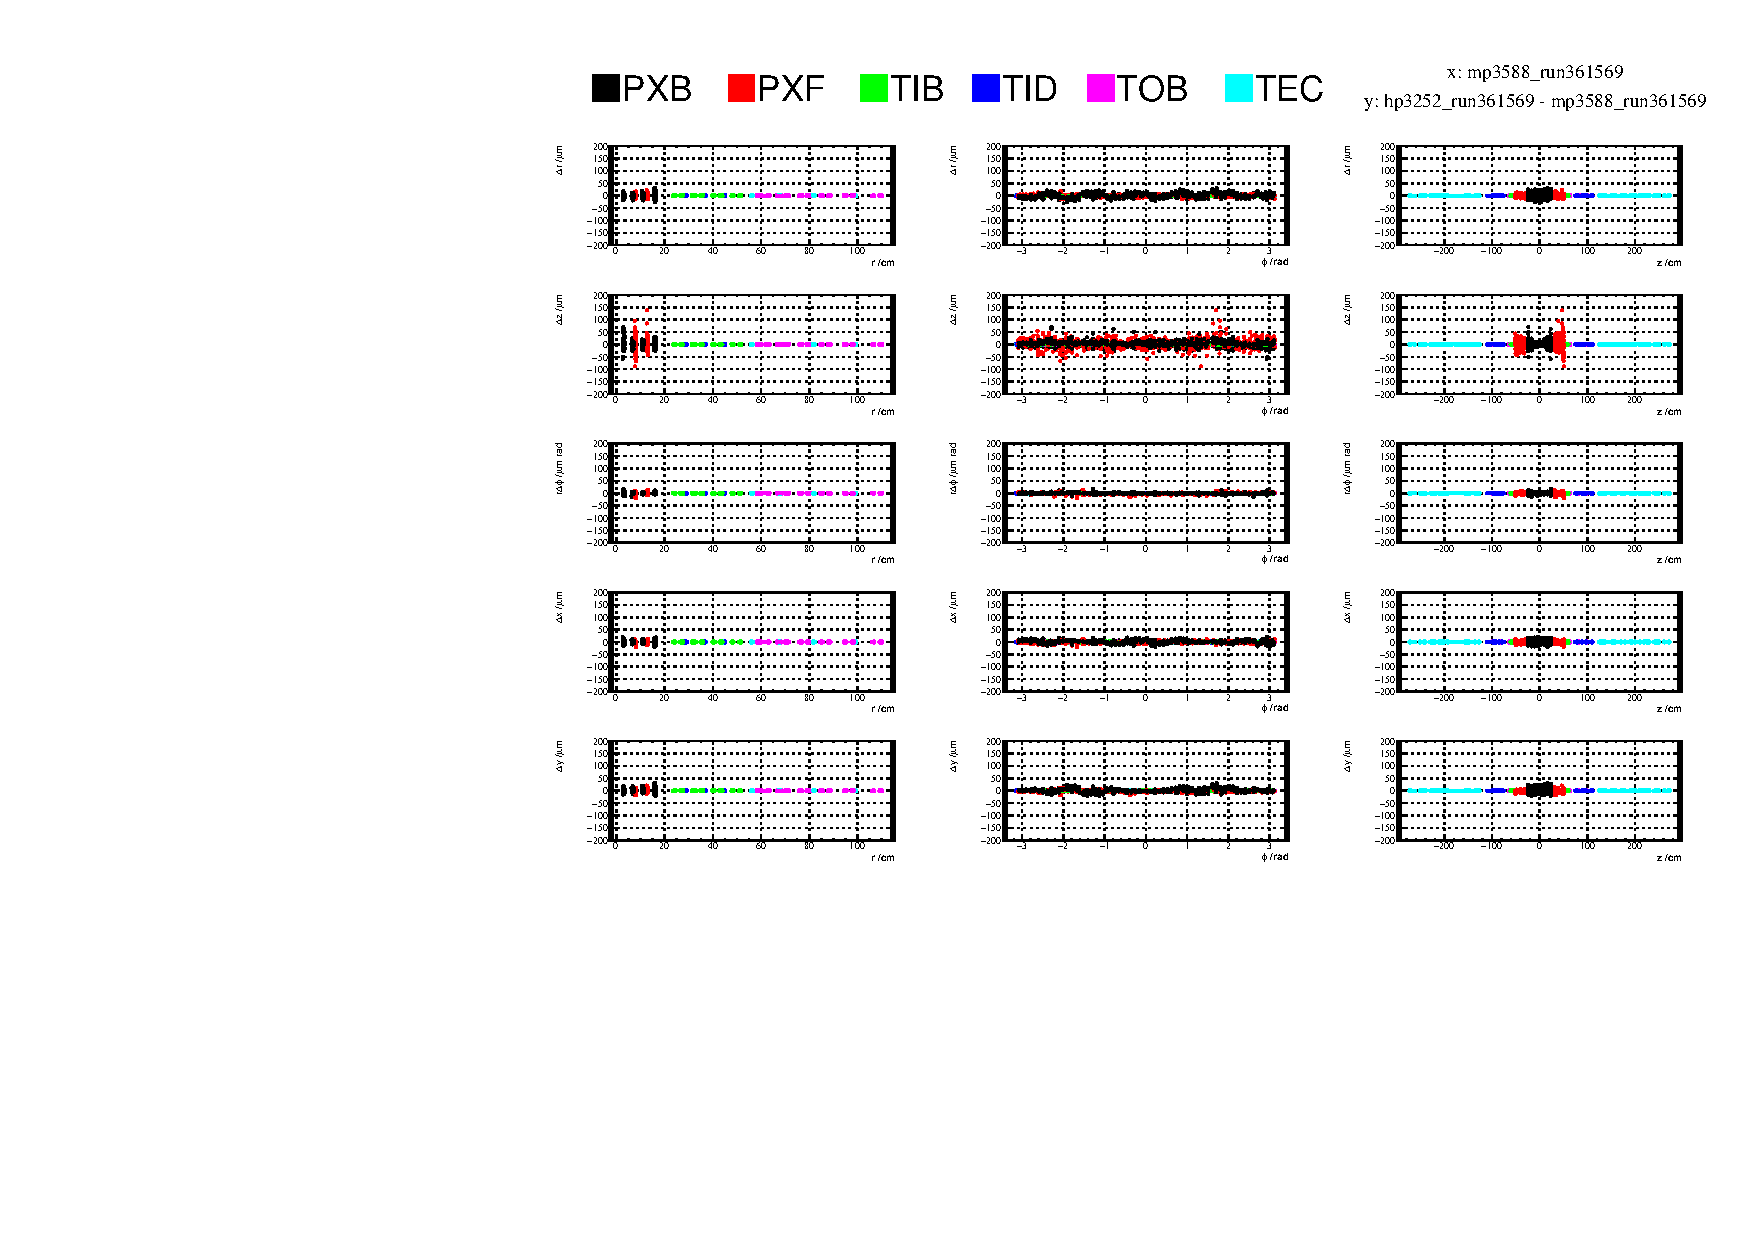
\includegraphics[width=1\textwidth] {global_tracker_1_final.pdf}
        \caption{Example global tracker plot for GC validation, comparing analogous HipPy and Millepede alignments using beam data, both calculated from PromptGT.}
        % ~\cite{WeeklyTr66:online}
        \label{fig:global_tracker_1_final}
    \end{center}
\end{figure}

\subsubsection{Distribution of the Median of Residuals}

By analyzing each module individually, the distributions of the median of residuals (DMRs) provide a measure of alignment improvement across subdetectors. This method involves refitting each track using all hits except for the one associated with the module under study. The residual, defined as the difference between the predicted and measured hit positions, is computed for each track, and the median of this distribution serves as a representative statistic for the module. These median residuals are then plotted across all modules, allowing for a comprehensive alignment evaluation.

To study various sources of bias, DMR validation is performed separately for the local \( x \) and \( y \) coordinates. A well-aligned detector should produce a DMR distribution centered around zero, with its width reflecting the statistical precision of the alignment (assuming a large enough sample of hits is used for validation). Deviations from zero suggest systematic biases, while a broader width indicates limitations in alignment accuracy. Since the width also depends on the sample size, valid comparisons require that all datasets have identical track statistics, as ensured in the validation process. Examples of DMR validation are shown in Figures~\ref{fig:DmedianR_BPIX_plain},~\ref{fig:DmedianR_FPIX_plain},~\ref{fig:DmedianYR_BPIX_plain},~\ref{fig:DmedianYR_FPIX_plain},~and~\ref{fig:2023_CRUZET_BPIX}.

\begin{figure}[!hbt]
    \begin{center}
        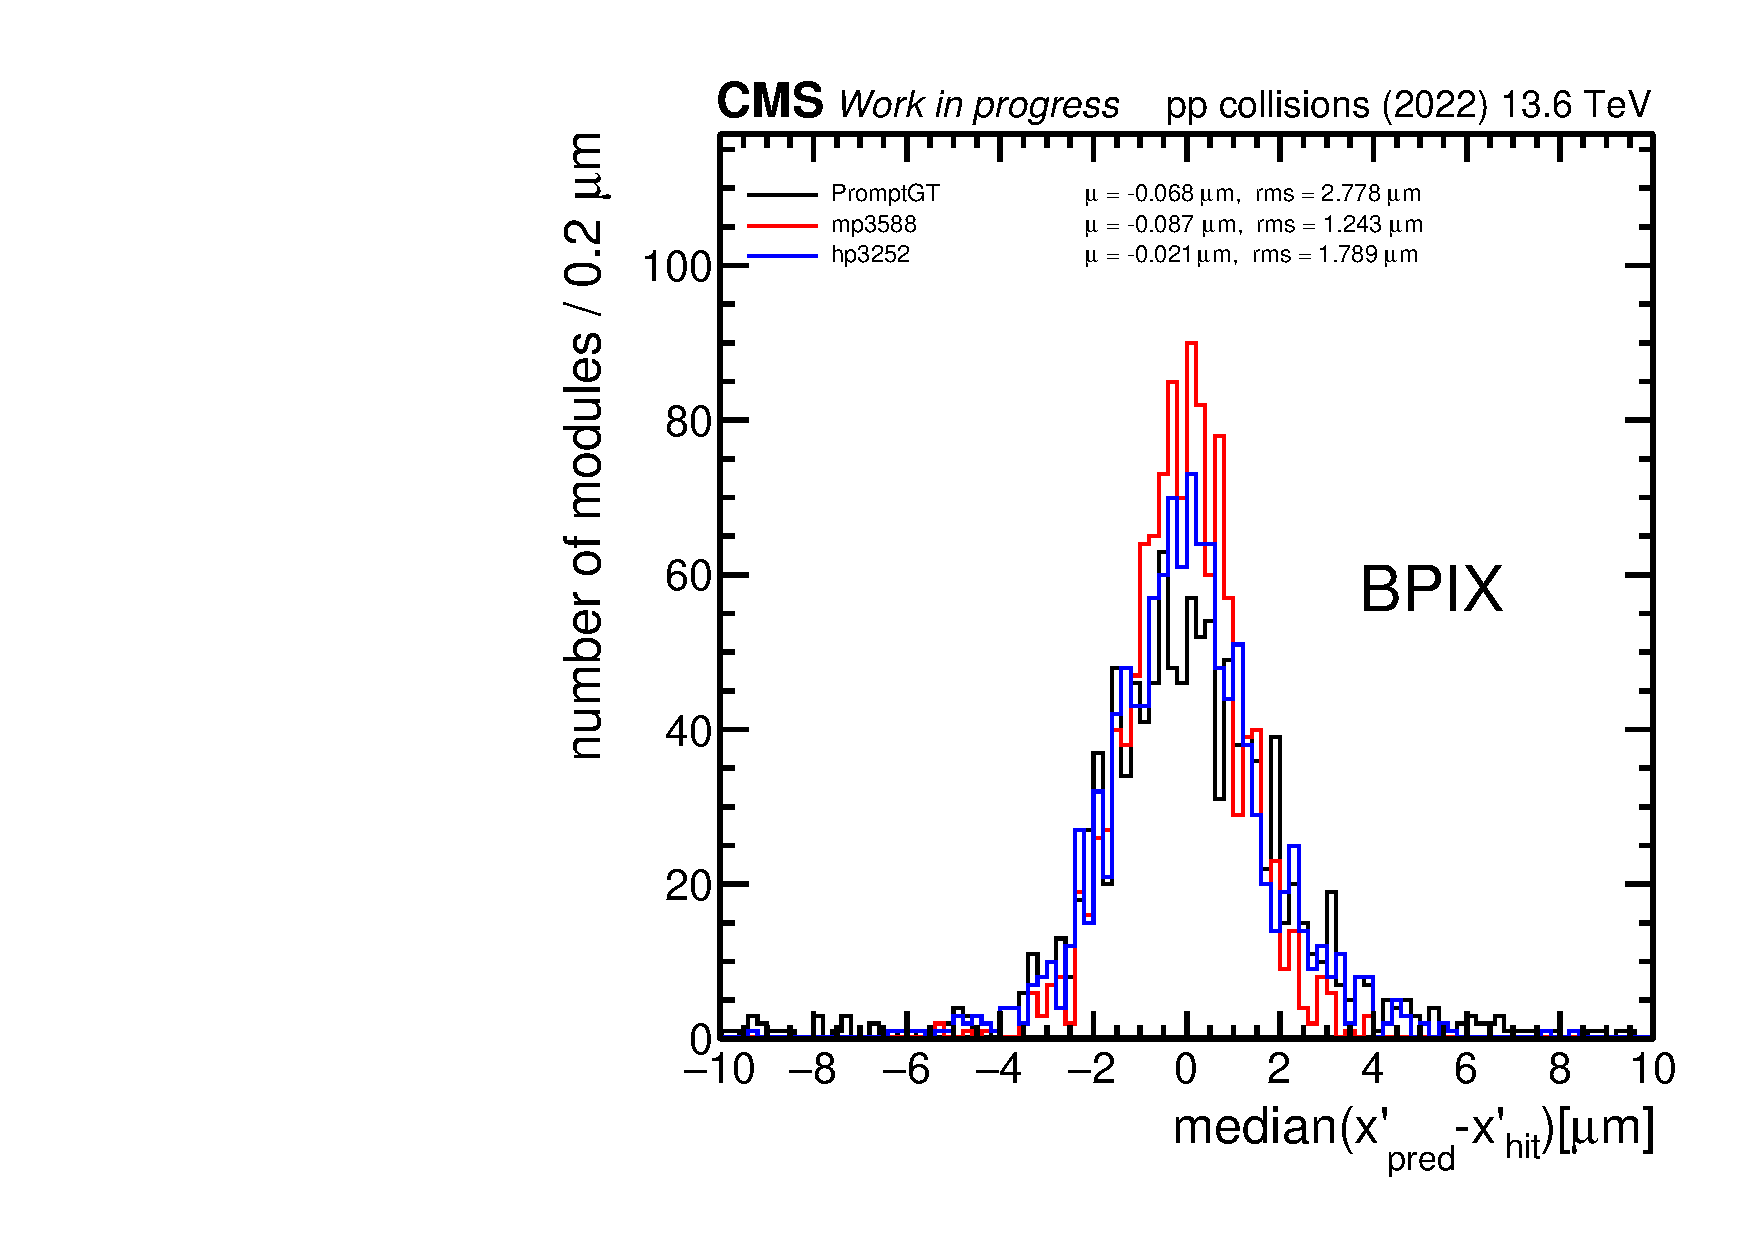
\includegraphics[width=0.9\textwidth,clip] {DmedianR_BPIX_plain.pdf}
        \caption{Example DMR validation plot for x residual in the BPIX, comparing HipPy (blue) and Millepede (red) alignments using beam data, both calculated from the starting geometry of PromptGT (black).}
        % ~\cite{WeeklyTr66:online}
        \label{fig:DmedianR_BPIX_plain}
    \end{center}
\end{figure}
\begin{figure}[!hbt]
    \begin{center}
        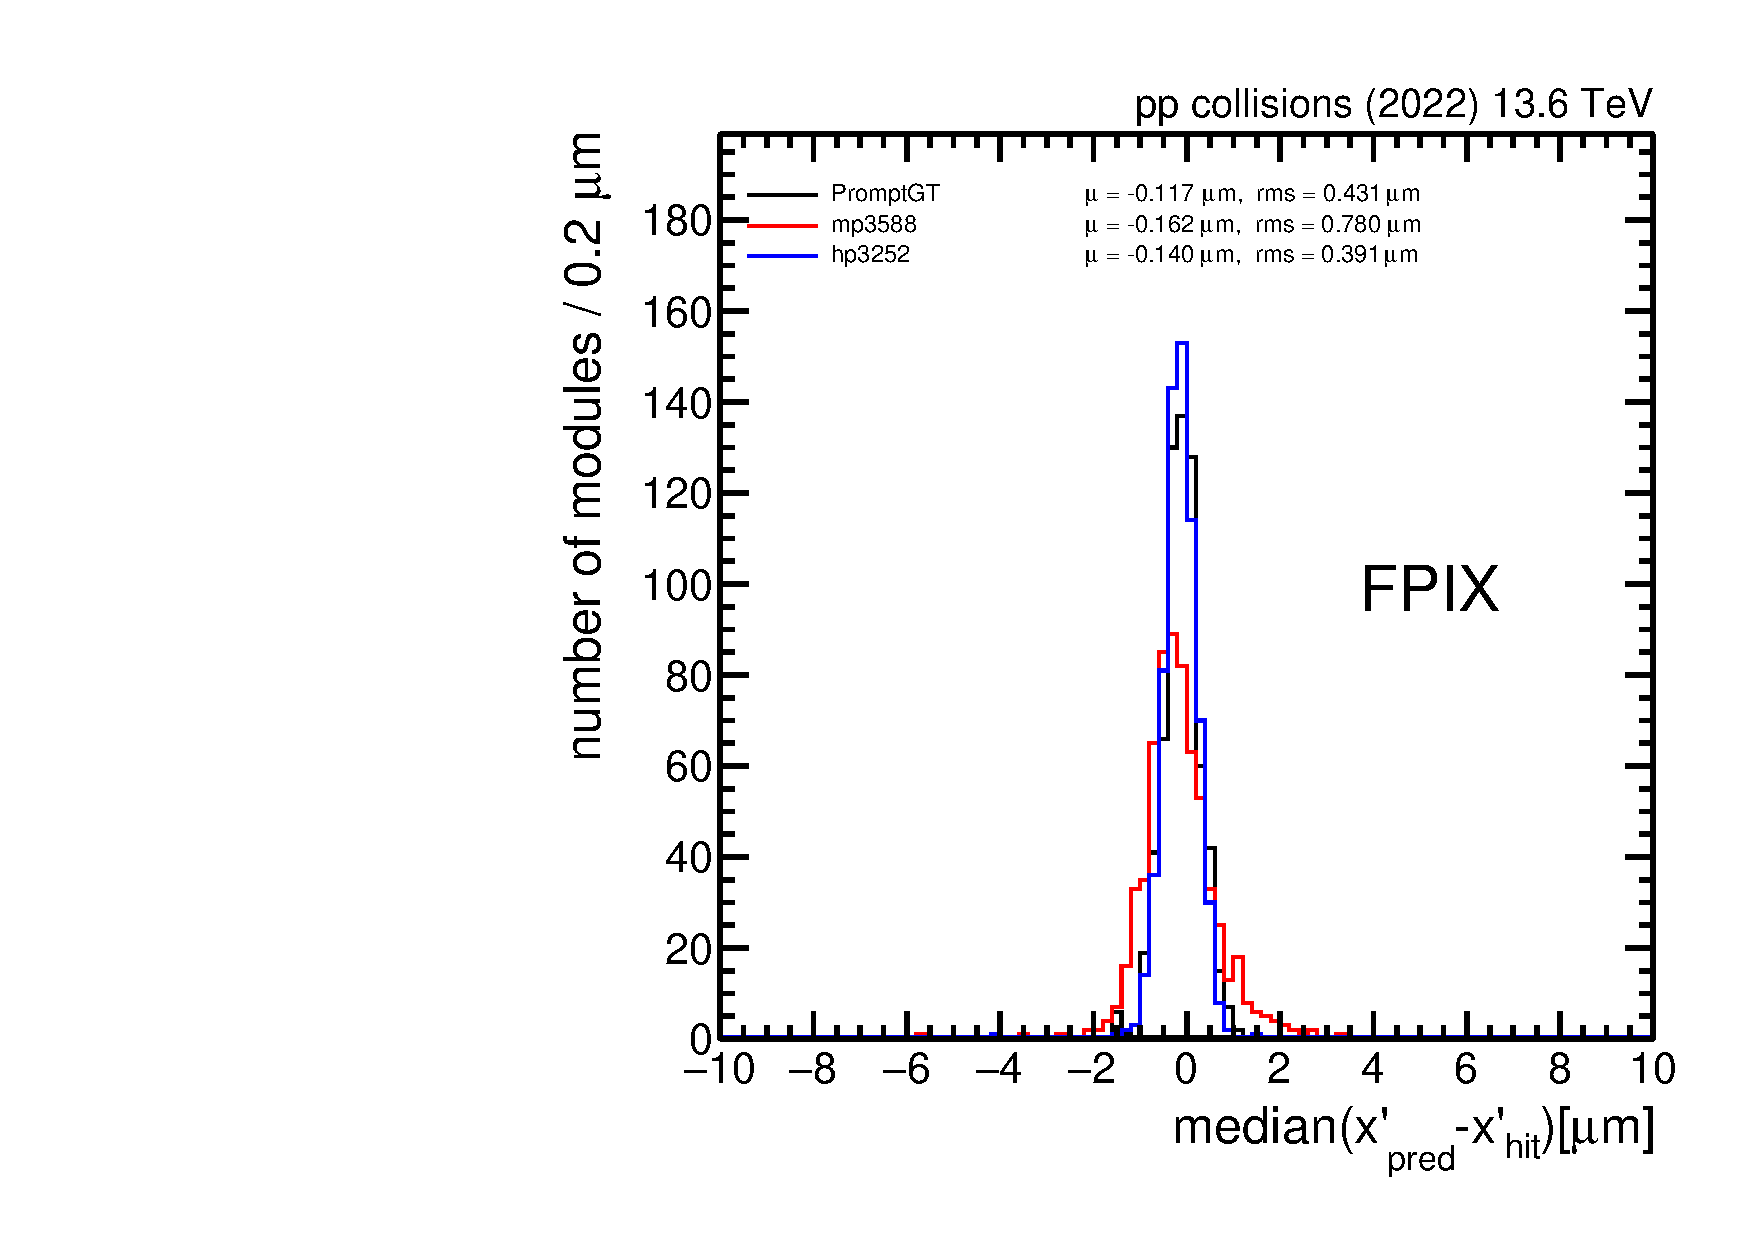
\includegraphics[width=0.9\textwidth,clip] {DmedianR_FPIX_plain.pdf}
        \caption{Example DMR validation plot for x residual in the FPIX, comparing HipPy (blue) and Millepede (red) alignments using beam data, both calculated from the starting geometry of PromptGT (black).}
        % ~\cite{WeeklyTr66:online}
        \label{fig:DmedianR_FPIX_plain}
    \end{center}
\end{figure}
\begin{figure}[!hbt]
    \begin{center}
        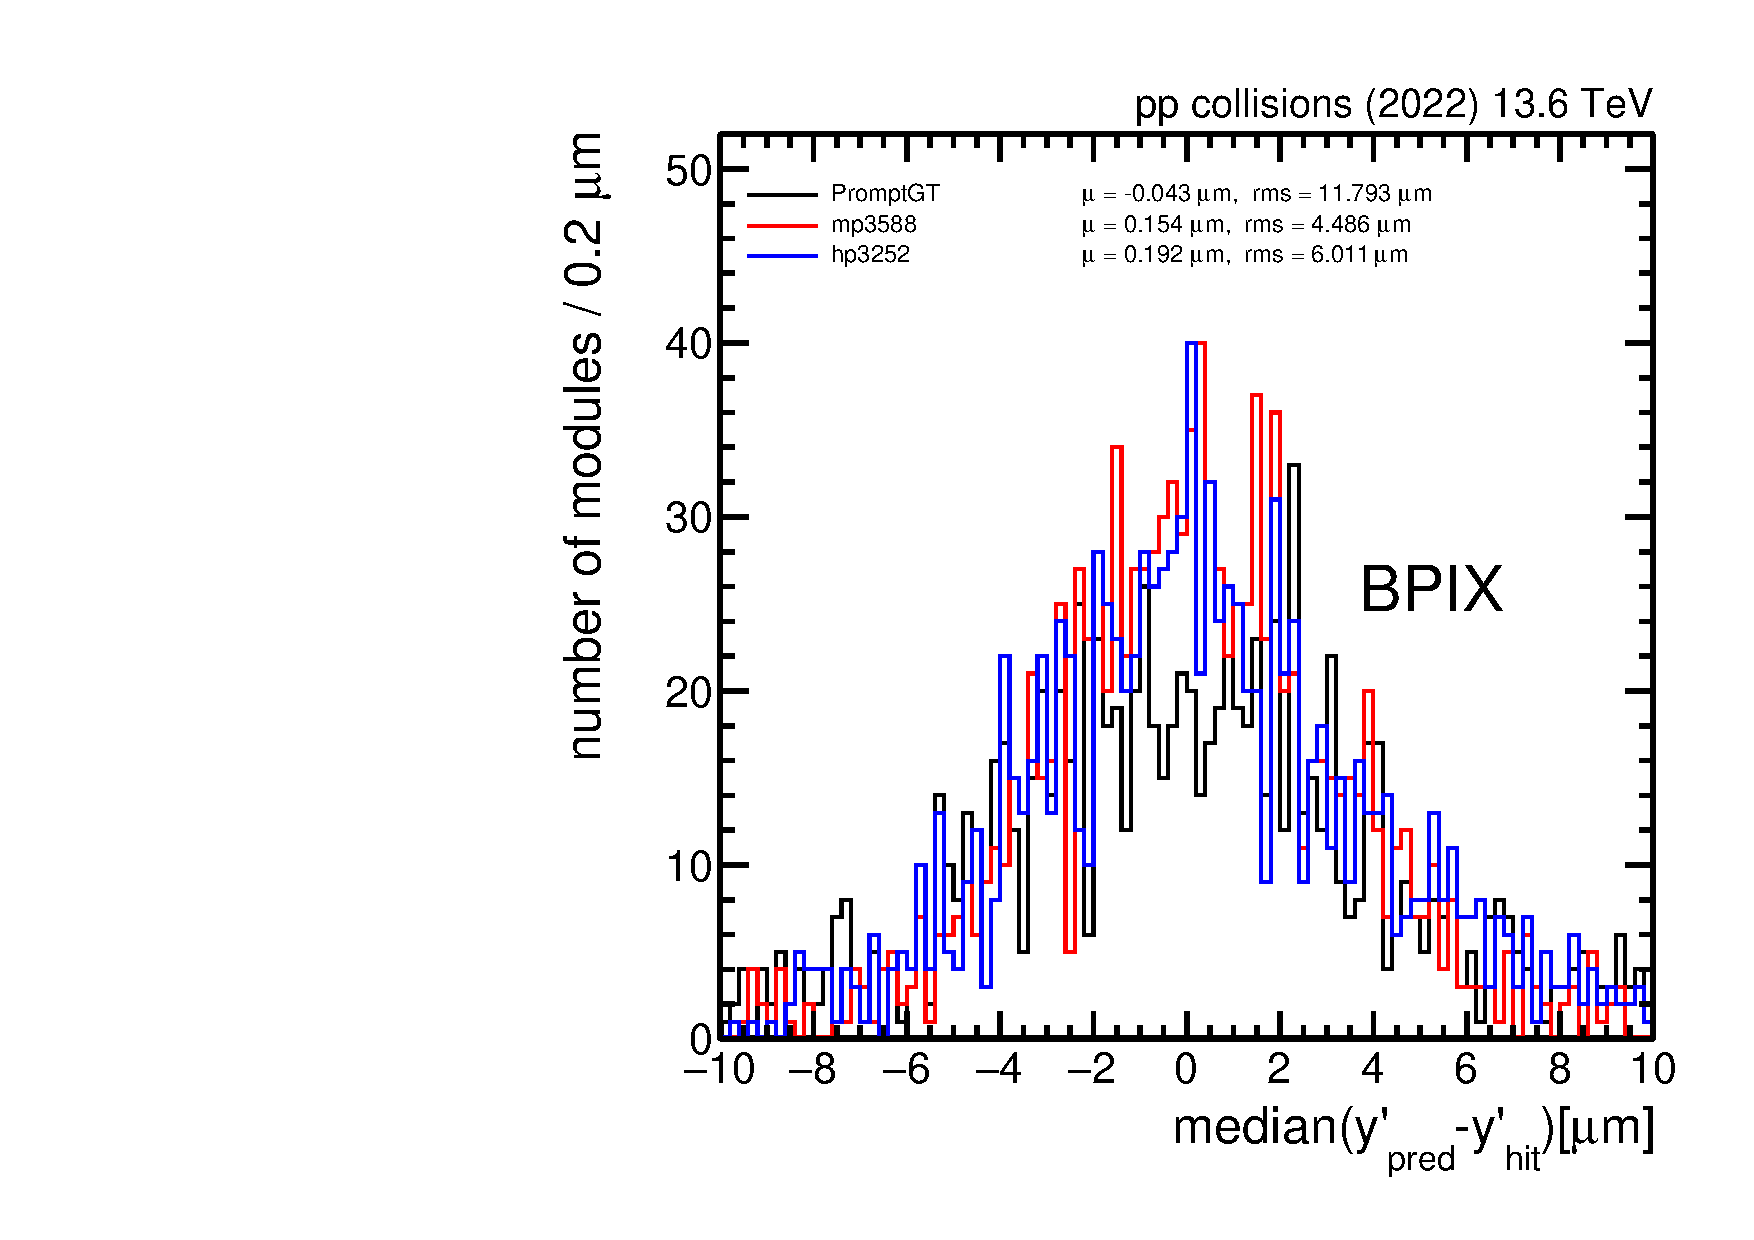
\includegraphics[width=0.9\textwidth,clip] {DmedianYR_BPIX_plain.pdf}
        \caption{Example DMR validation plot for y residual in the BPIX, comparing HipPy (blue) and Millepede (red) alignments using beam data, both calculated from the starting geometry of PromptGT (black).}
        % ~\cite{WeeklyTr66:online}
        \label{fig:DmedianYR_BPIX_plain}
    \end{center}
\end{figure}
\begin{figure}[!hbt]
    \begin{center}
        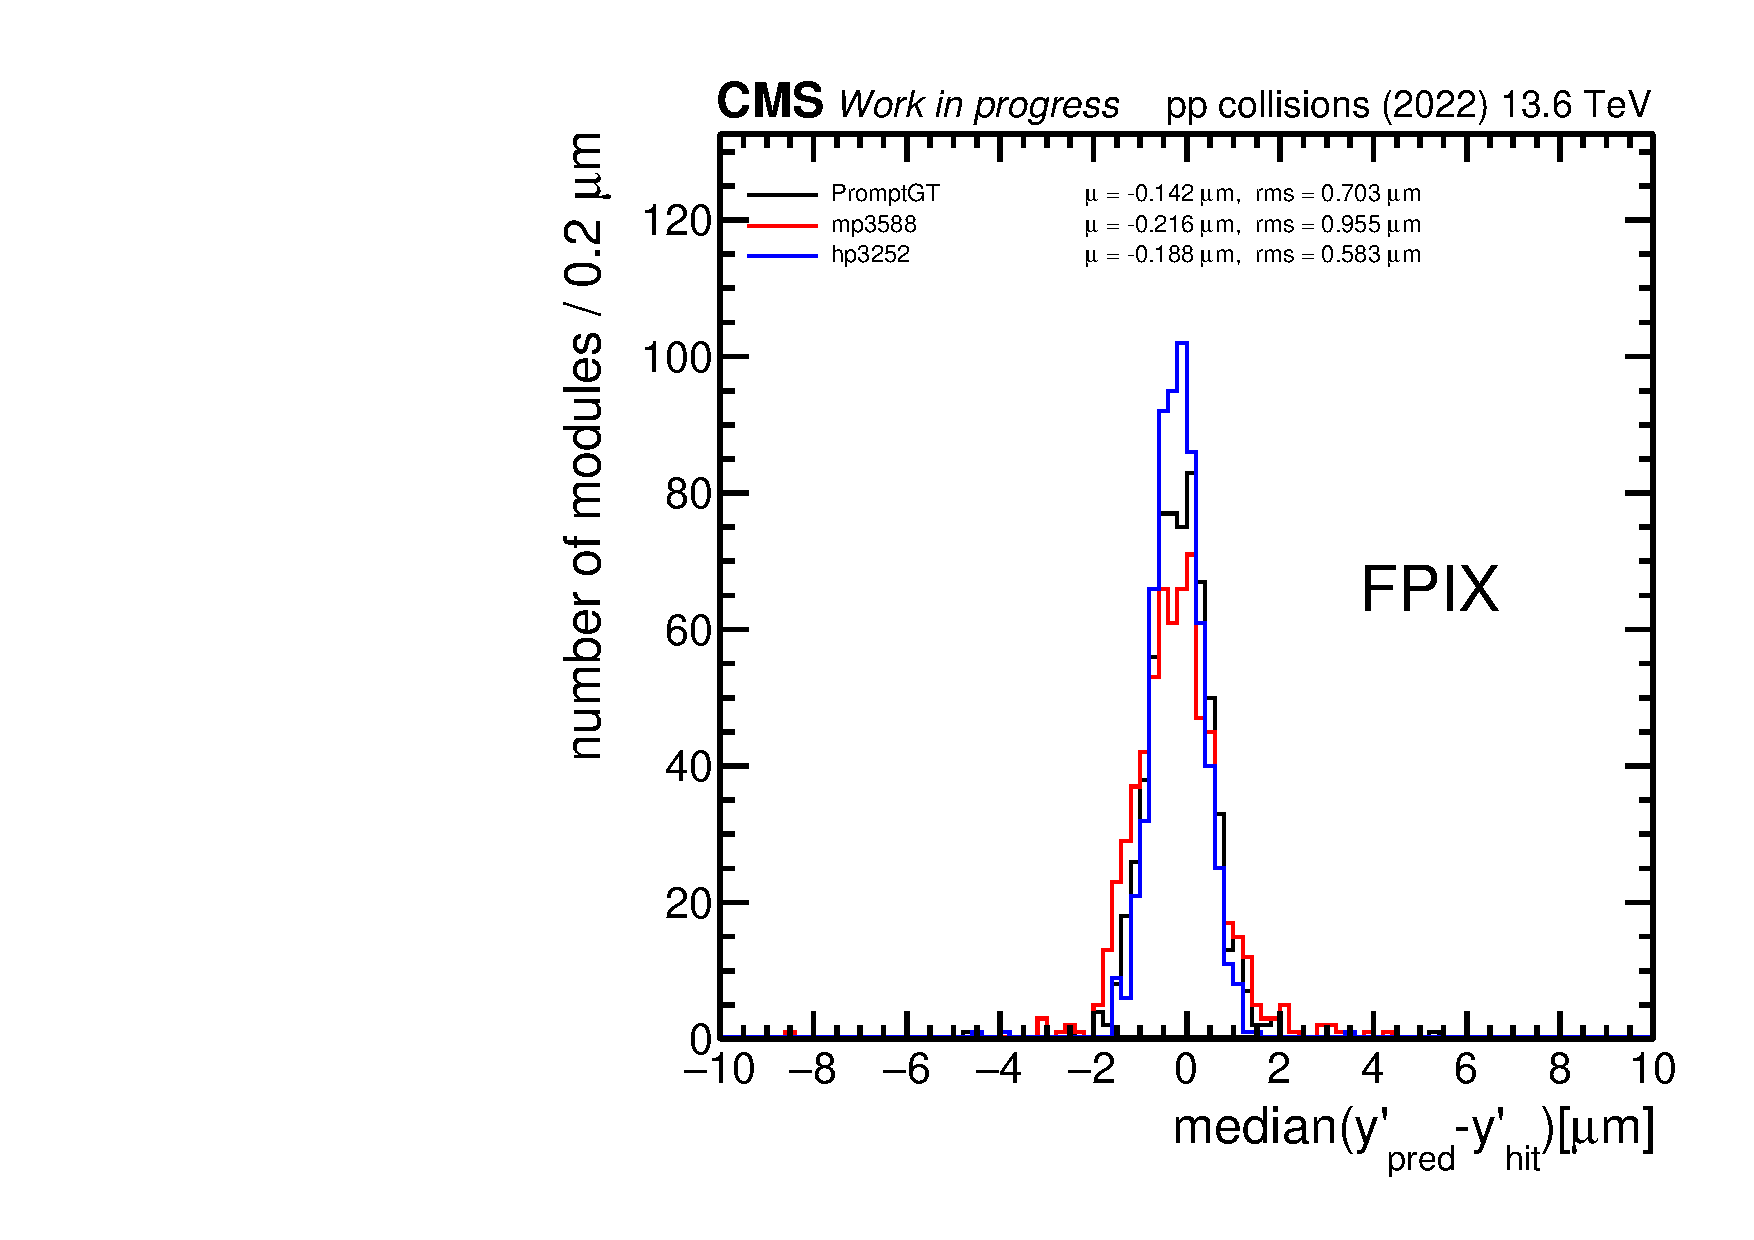
\includegraphics[width=0.9\textwidth,clip] {DmedianYR_FPIX_plain.pdf}
        \caption{Example DMR validation plot for y residual in the FPIX, comparing HipPy (blue) and Millepede (red) alignments using beam data, both calculated from the starting geometry of PromptGT (black).}
        % ~\cite{WeeklyTr66:online}
        \label{fig:DmedianYR_FPIX_plain}
    \end{center}
\end{figure}

\subsubsection{Primary Vertex}

The quality of tracker alignment is further assessed through its impact on the performance of physics objects, particularly the reconstruction of the primary vertex (PV). The PV, typically defined as the vertex associated with the track of highest transverse momentum (\( p_T \)), is primarily determined by the pixel detector, as it is closest to the interaction point and offers the best intrinsic hit position resolution. 

The precision of vertex reconstruction is evaluated using unbiased track-vertex residuals, also known as track impact parameters, which provide a direct measurement based on data. For each track, the PV position is reconstructed while excluding the track under consideration. To ensure robustness against pileup, a deterministic annealing clustering algorithm is utilized. Examples of PV validation are shown in Figures~\ref{fig:BiasesCanvas_PromptGT_vs_mp3588_vs_hp3252}~and~\ref{fig:BiasesCanvasLayer1_PromptGT_vs_mp3588_vs_hp3252}.

\begin{figure}[!hbt]
    \begin{center}
        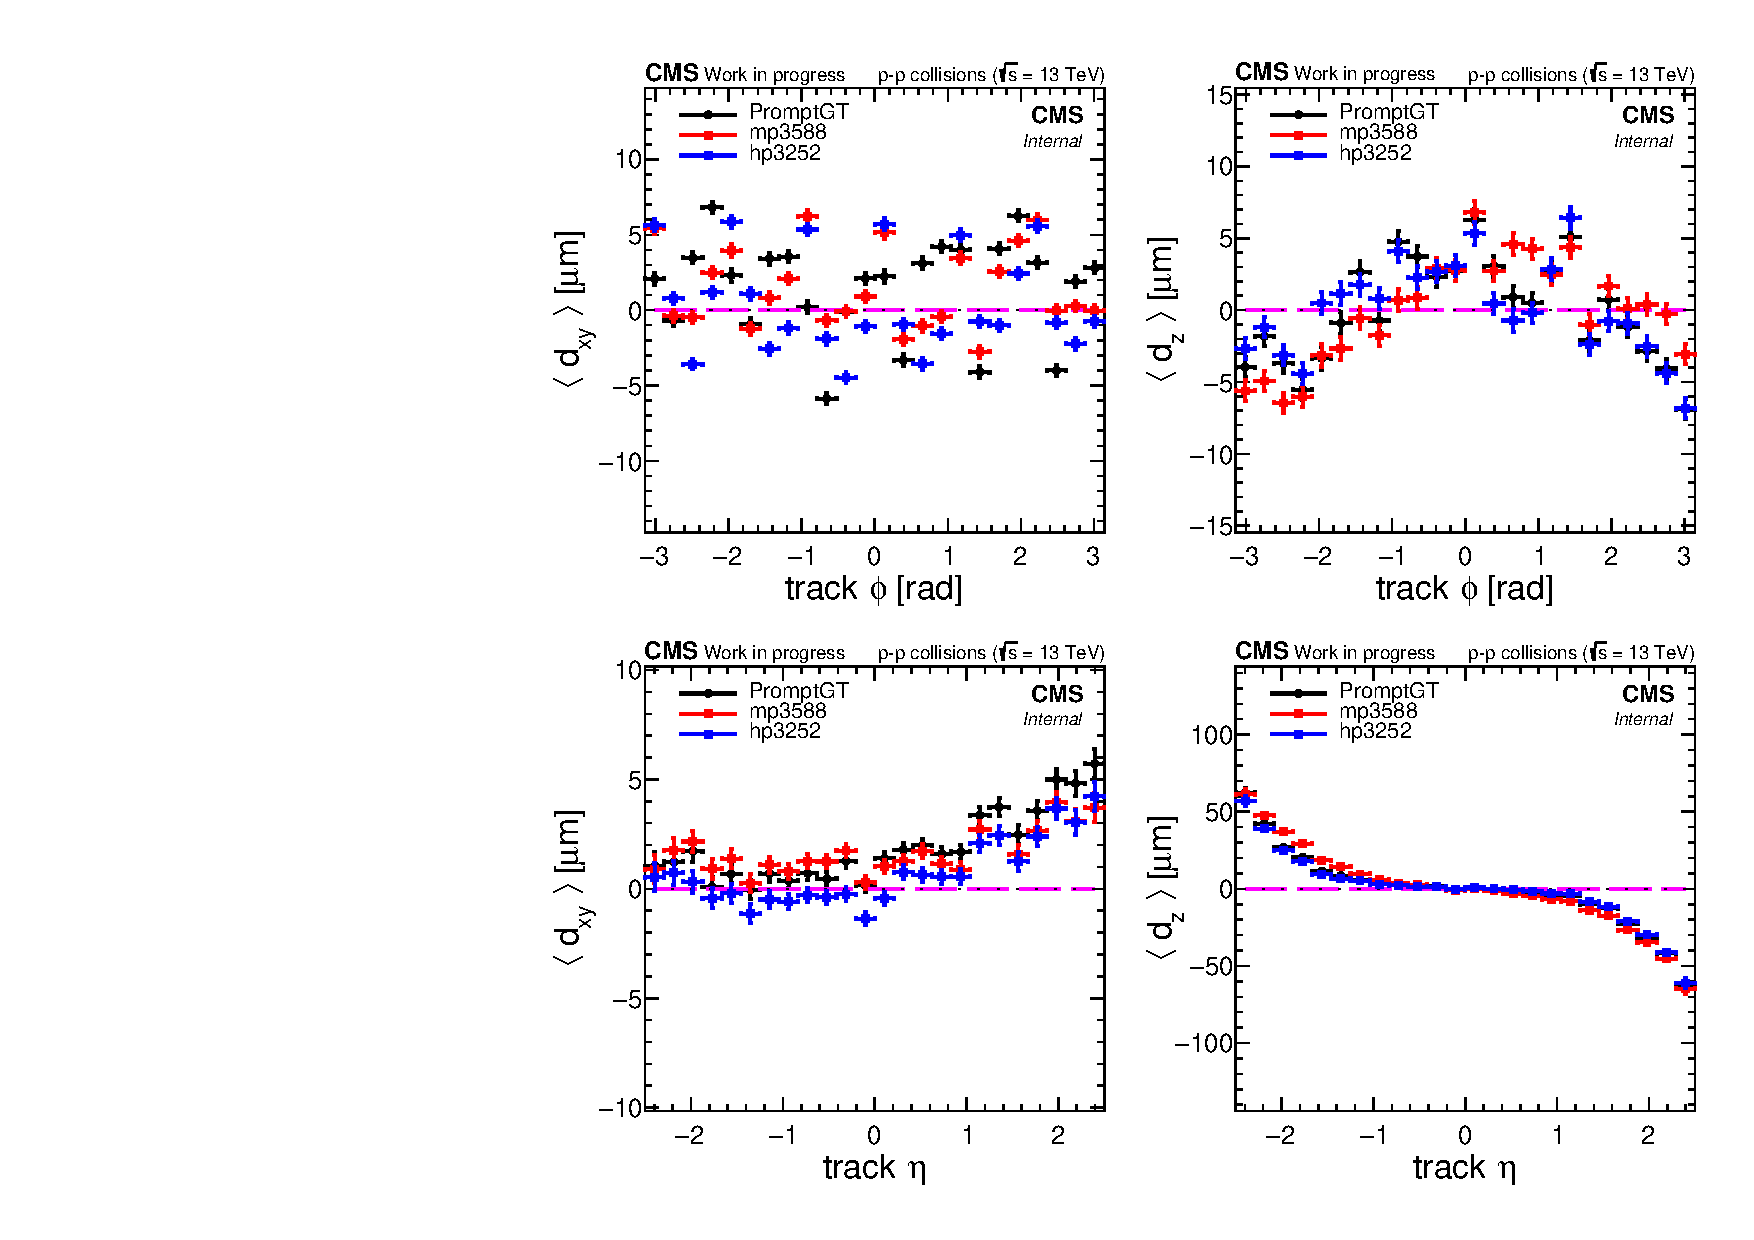
\includegraphics[width=0.9\textwidth,clip] {BiasesCanvas_PromptGT_vs_mp3588_vs_hp3252.pdf}
        \caption{Example PV validation plot for PIX, comparing HipPy (blue) and Millepede (red) alignments using beam data, both calculated from the starting geometry of PromptGT (black).}
        % ~\cite{WeeklyTr66:online}
        \label{fig:BiasesCanvas_PromptGT_vs_mp3588_vs_hp3252}
    \end{center}
\end{figure}
\begin{figure}[!hbt]
    \begin{center}
        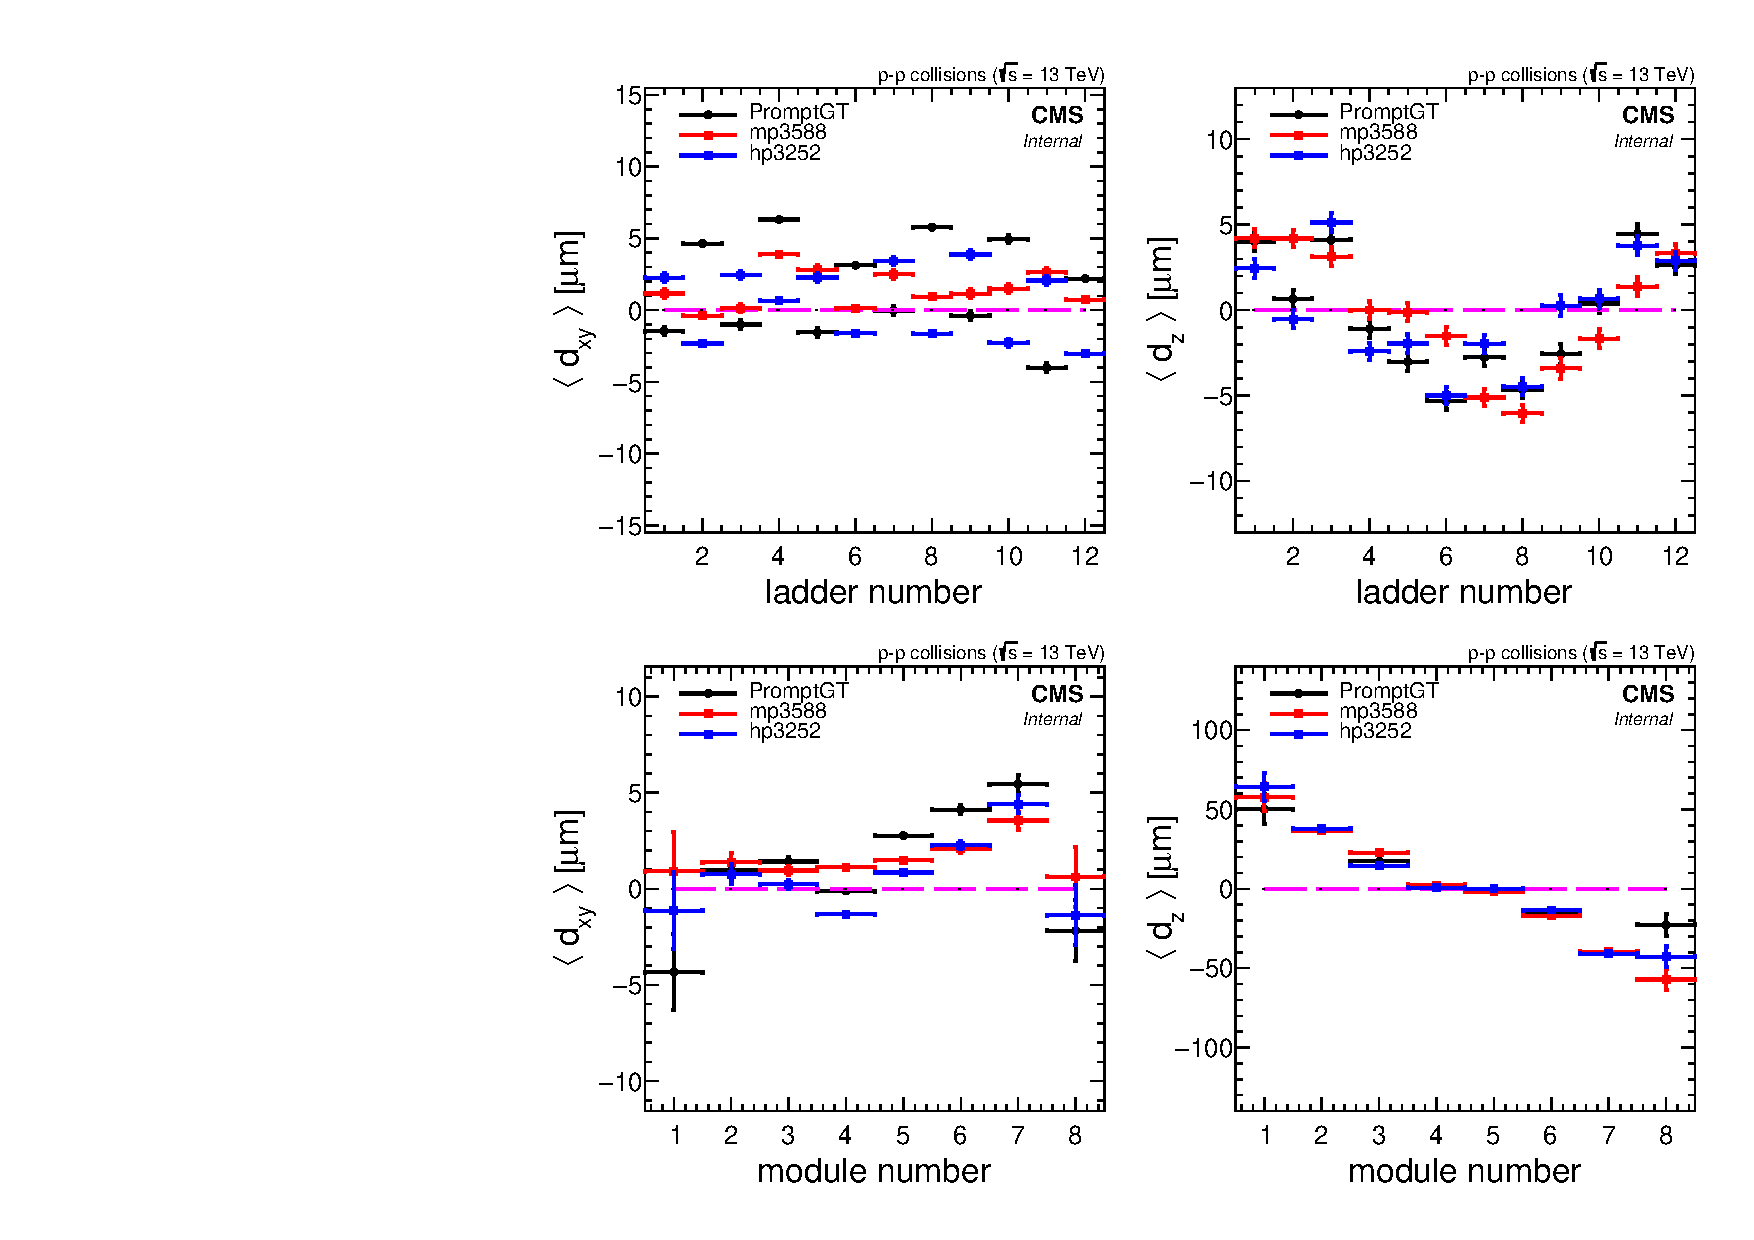
\includegraphics[width=0.9\textwidth,clip] {BiasesCanvasLayer1_PromptGT_vs_mp3588_vs_hp3252.pdf}
        \caption{Example PV validation plot for BPIX Layer 1, comparing HipPy (blue) and Millepede (red) alignments using beam data, both calculated from the starting geometry of PromptGT (black).}
        % ~\cite{WeeklyTr66:online}
        \label{fig:BiasesCanvasLayer1_PromptGT_vs_mp3588_vs_hp3252}
    \end{center}
\end{figure}

\subsubsection{Cosmic Track Splitting}

Cosmic ray muons, often referred to as cosmics or cosmic events, recorded by the CMS detector are used for detector commissioning and calibration. Before the magnetic field is turned on, events are recorded during the Cosmic RUns at ZEro Tesla (CRUZET). Cosmic ray muon tracks are also recorded in the 3.8 T magnetic field provided by the CMS solenoid during the Cosmic Runs At Four Tesla (CRAFT).

Tracks from cosmic ray muons are crucial for deriving alignment constants for two main reasons. First, they can be recorded before the start of LHC collisions and are therefore used to derive the initial alignment corrections after a shutdown period. Second, they have a very different topology compared to collision tracks. Unlike collision tracks, cosmic ray muon tracks traverse the entire detector and connect modules in the top and bottom halves of the tracker. This breaks the cylindrical symmetry typical of collision tracks and helps to constrain several types of distortions.

Throughout Run 2, cosmic ray muon events were recorded before the start of LHC collisions during dedicated commissioning runs and in the time intervals between two LHC fills (interfill runs). Since 2018, cosmic events have also been recorded during collision data-taking.

\begin{figure}[!hbt]
\centering
\begin{subfigure}[t]{0.37\textwidth}
    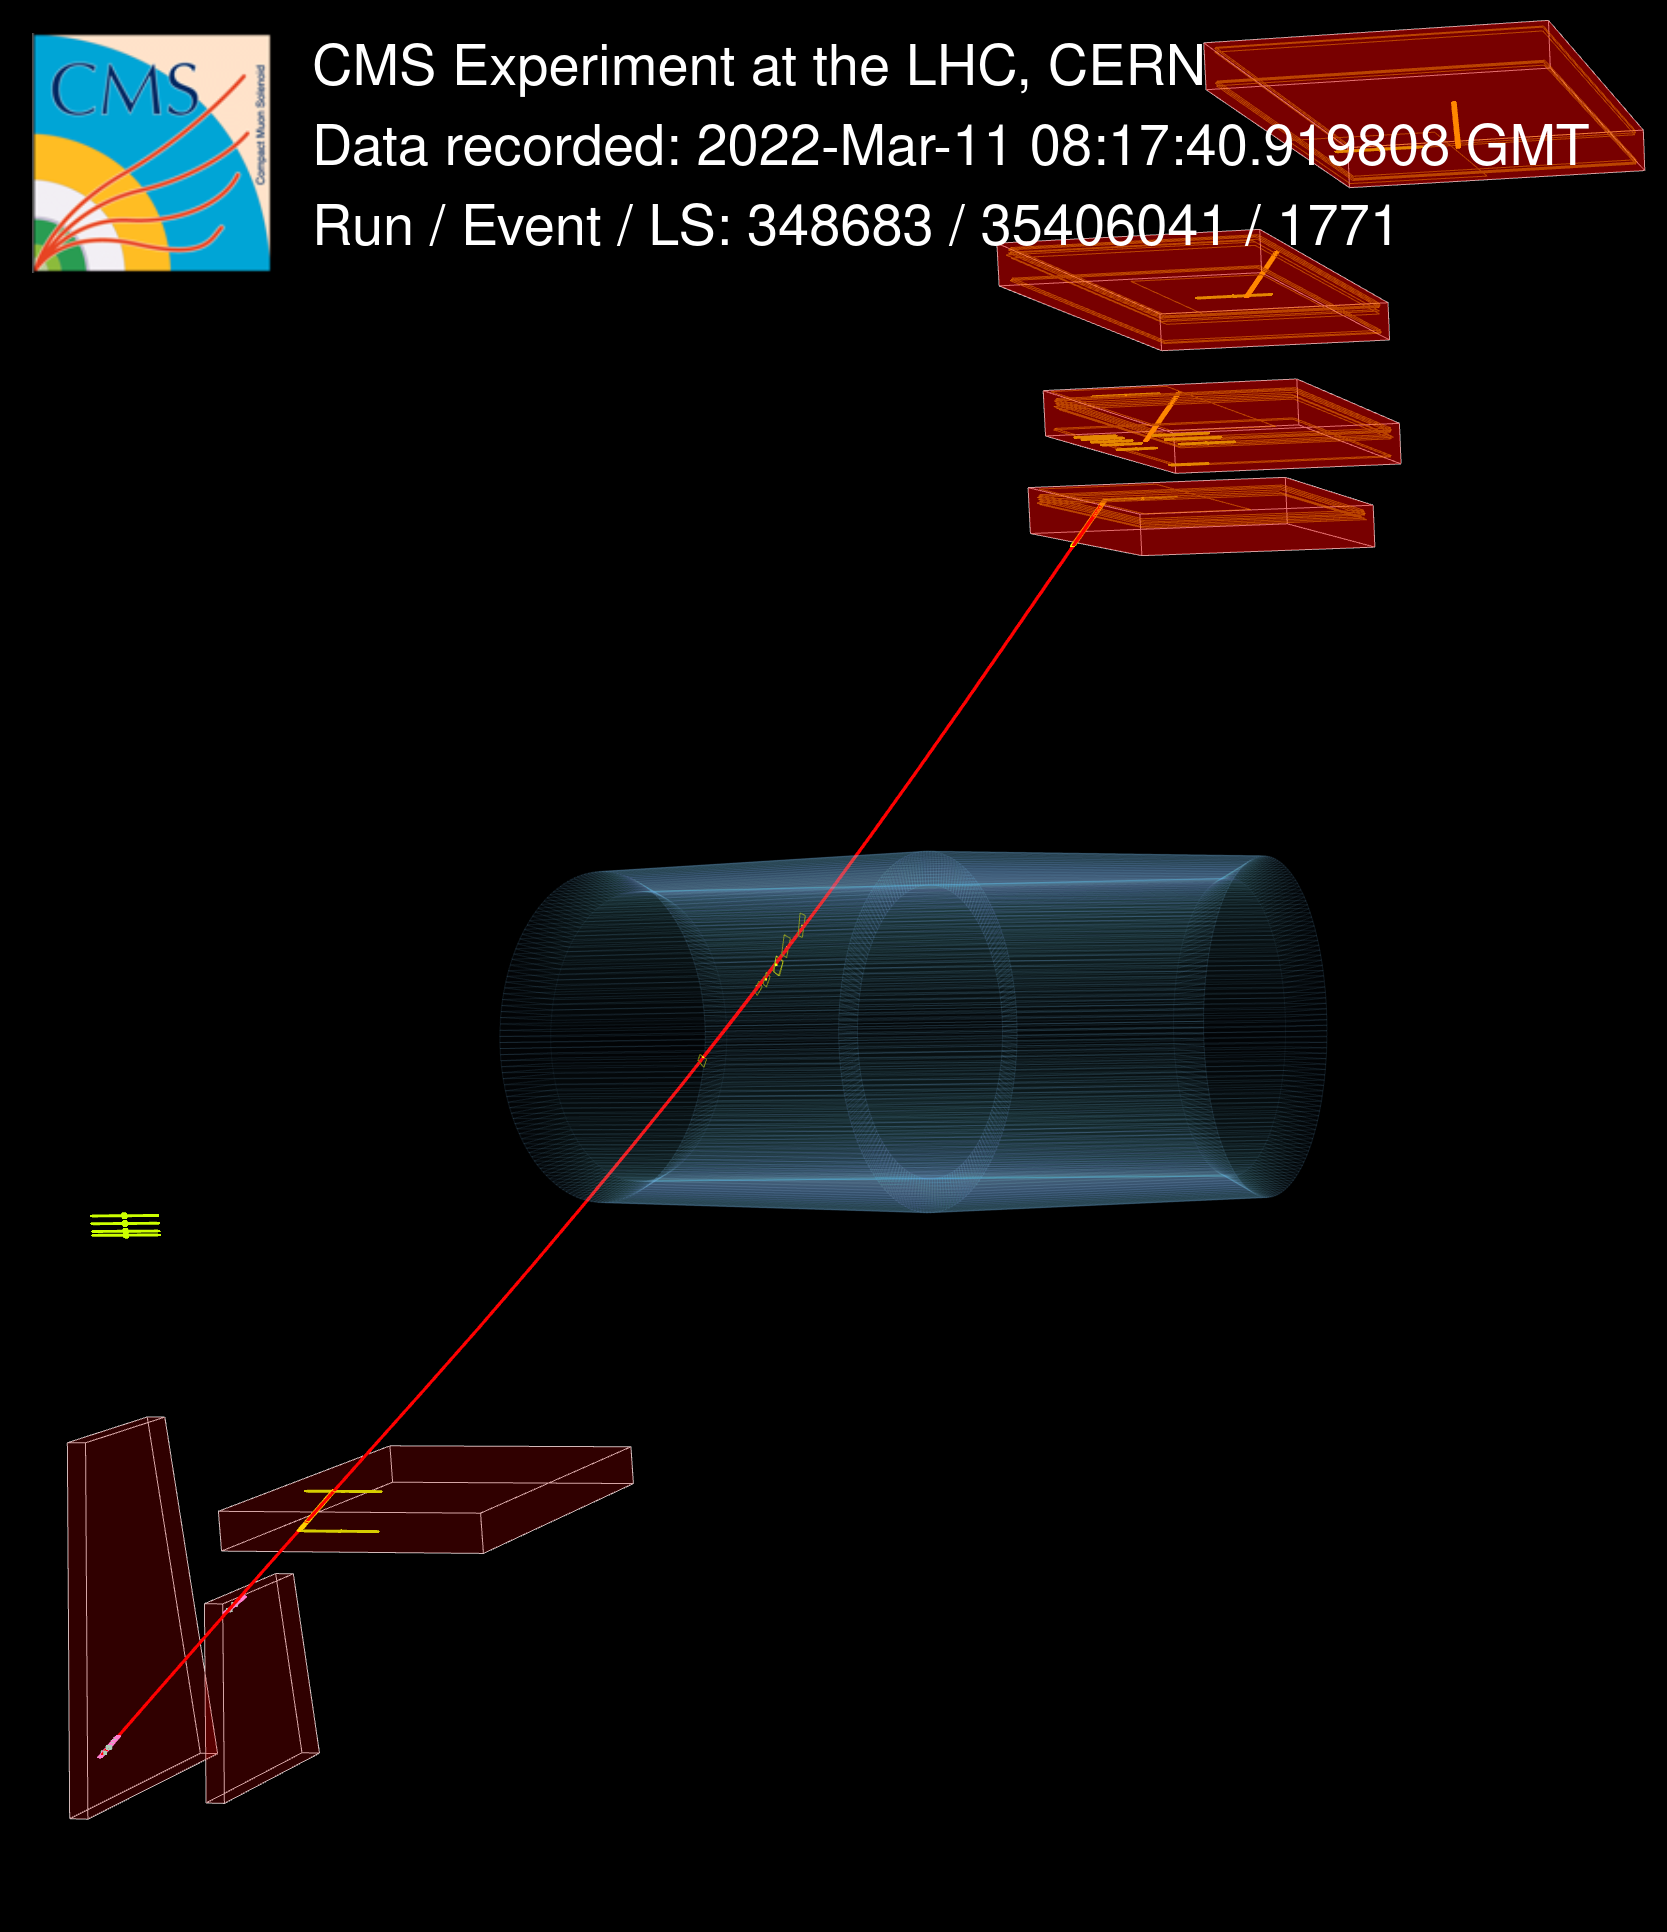
\includegraphics[width=\textwidth]{figures/CRAFT-2022_1.png}
    \caption{}
    \label{fig:cosmicside}
\end{subfigure}
\begin{subfigure}[t]{0.53\textwidth}
    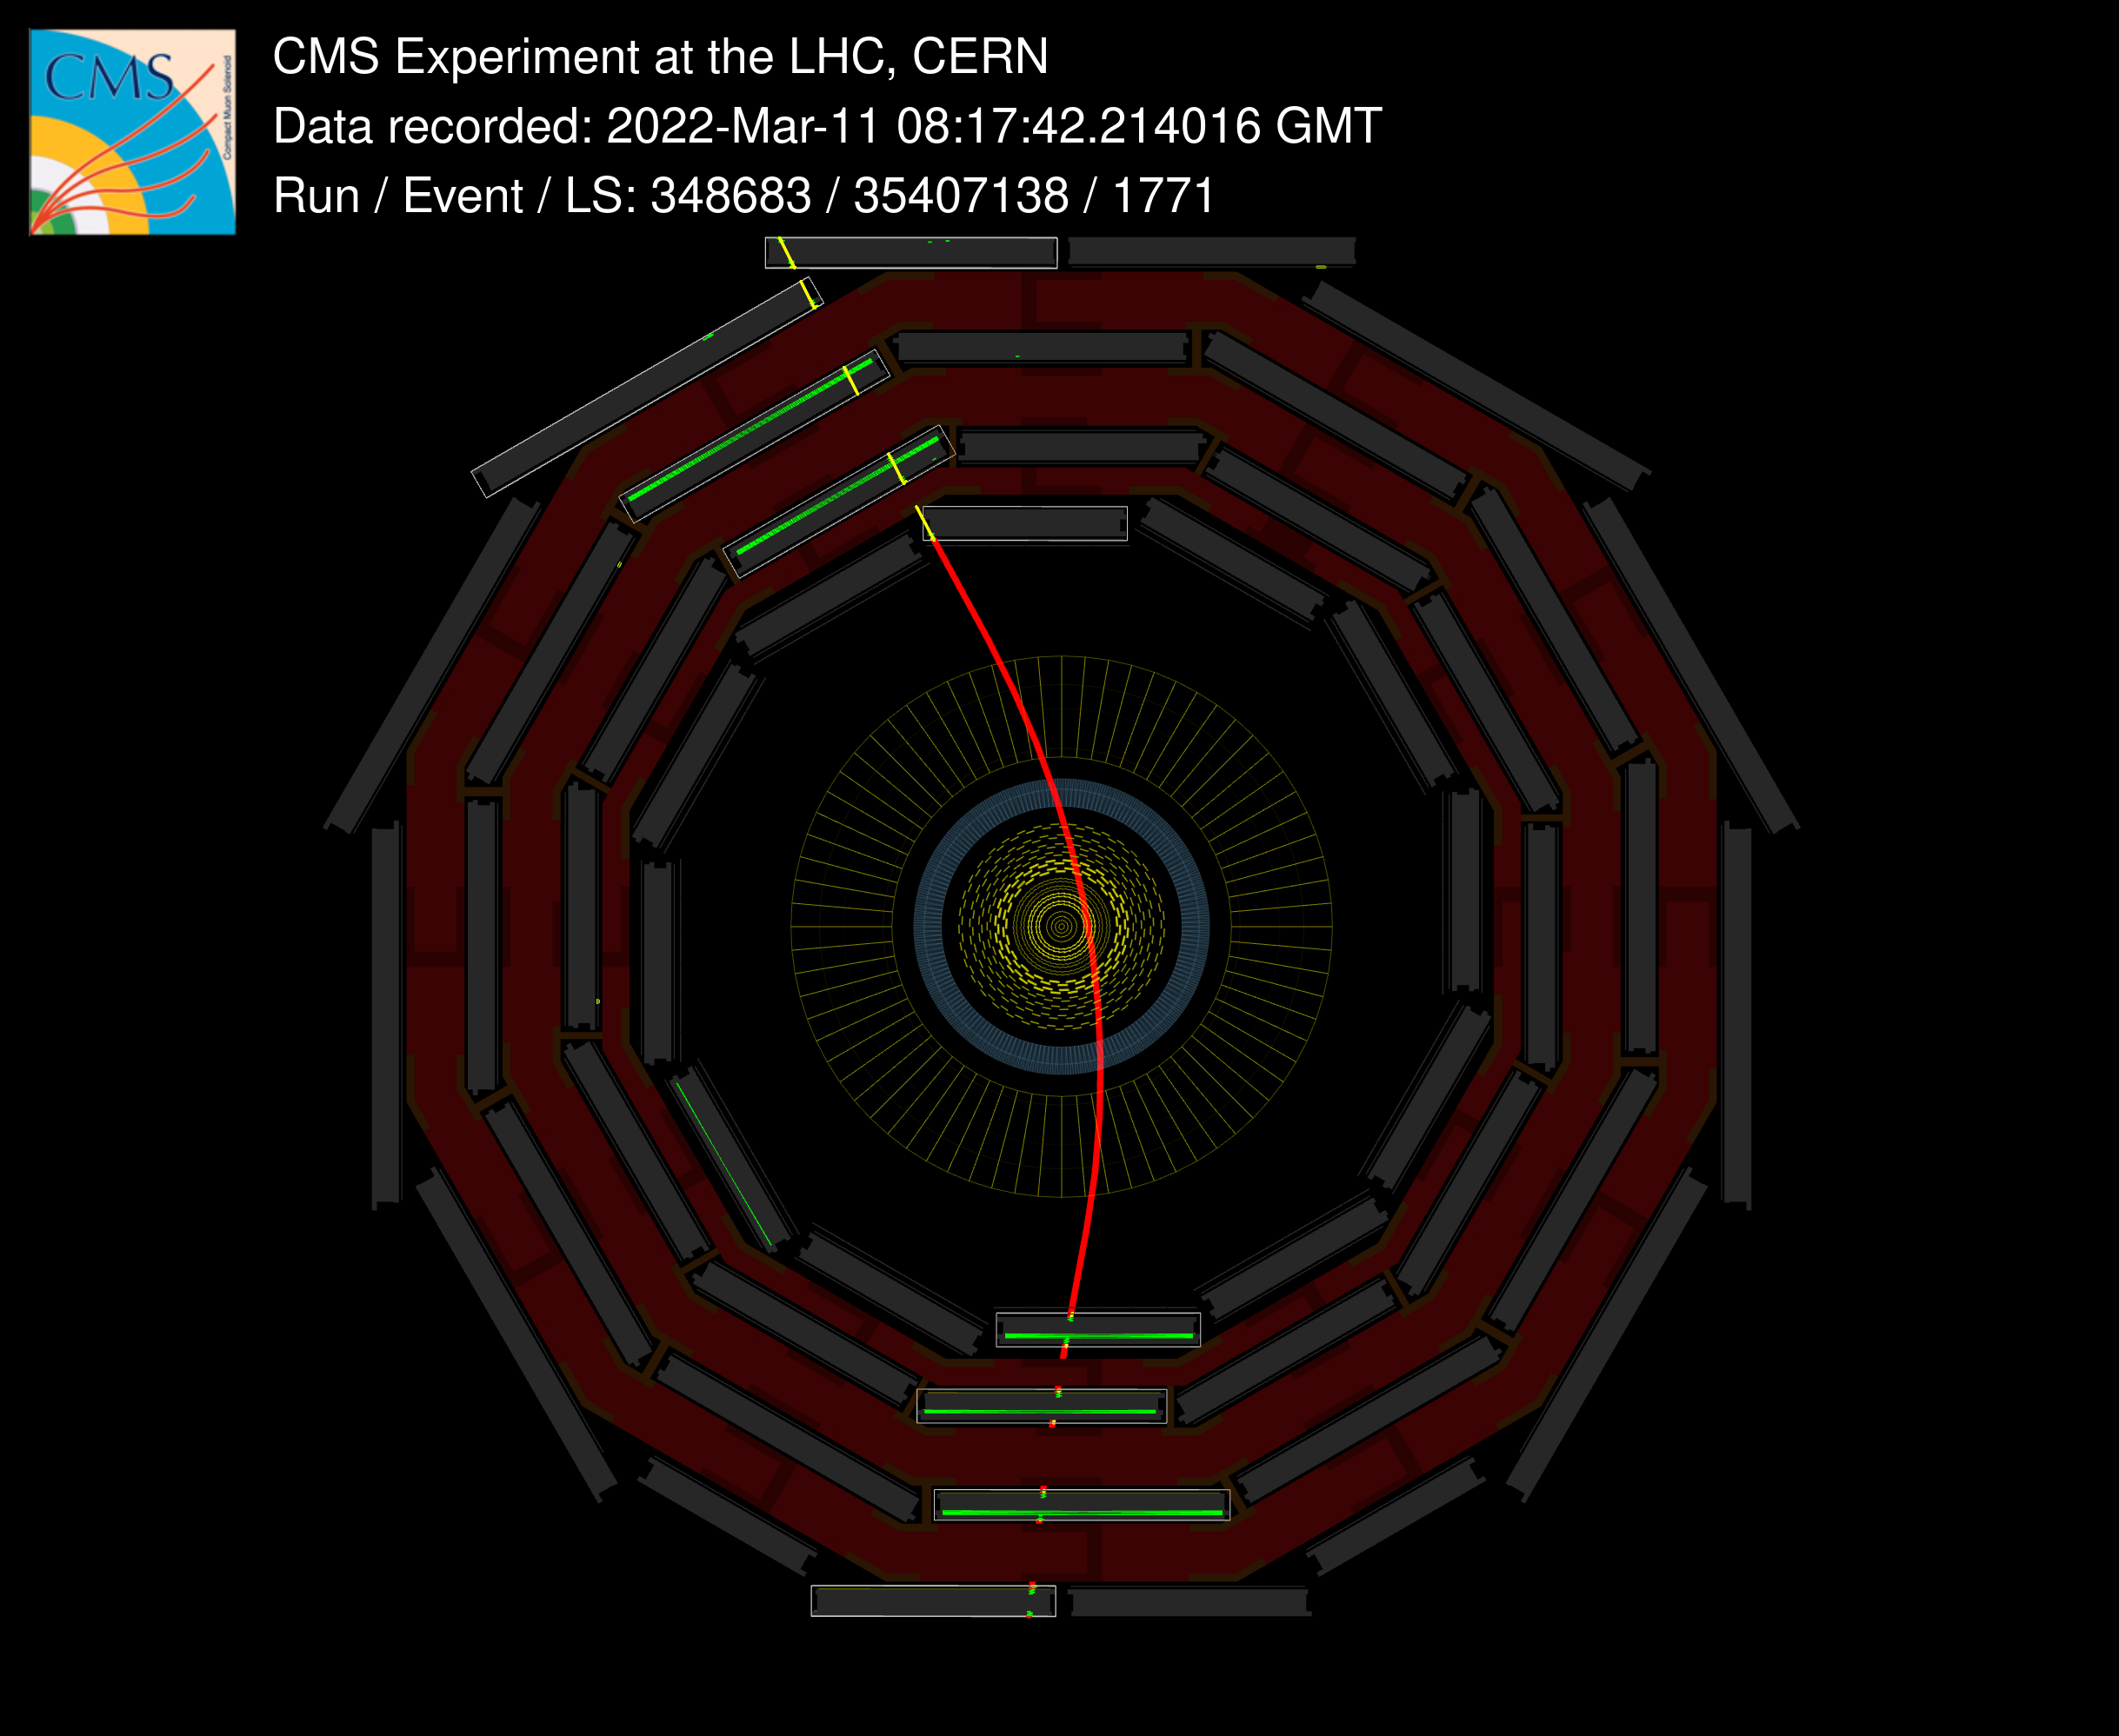
\includegraphics[width=\textwidth]{figures/CRAFT-2022_0.png}
    \caption{}
    \label{fig:cosmicfront}
\end{subfigure}
\caption{Muons generated by cosmic rays are extremely important for the commissioning and the alignment of CMS. Despite being 100 m underground, every second hundreds of muons generated on top of the atmosphere cross CMS. Presented are two views, transverse (left) and longitudinal (right), of a single cosmic ray event~\cite{Collaboration:2806755}.}
\label{fig:cosmicevent}
\end{figure}

% The resolution of track parameters can be validated using cosmic ray muon tracks by independently reconstructing the upper and lower segments of each track as it traverses the tracker. By comparing the track parameters at the point of closest approach to the nominal beamline, systematic differences between the two halves can indicate misalignment. This procedure is particularly powerful because the two halves of a given cosmic ray track should have identical parameters at the beamline, since they should form a straight line through the detector. Cosmic ray tracks effectively mimic standard collision tracks originating from the same point, but independent of beam collision data.

% Cosmic ray muon tracks and collision tracks exhibit distinct topologies, making them sensitive to different types of geometric distortions. Systematic deformations that manifest as weak modes in collision tracks may be well constrained or more easily identifiable using cosmic tracks. Since cosmic rays originate externally rather than from the interaction point, they connect the upper and lower halves of the tracker through a single continuous trajectory—a configuration not achievable with beam-induced tracks. This topology allows for precise constraints on the alignment of horizontal modules along the \(z\)-axis but provides limited sensitivity to vertical module misalignments in the endcap regions or modules spanning different horizontal sections of the detector.

% Cosmic ray muon track validation is particularly valuable before the start of LHC operations, as it allows for an initial assessment of detector alignment without requiring beam collision data. However, it remains a crucial diagnostic tool throughout data-taking periods due to the unique trajectory and independent constraints provided by cosmic ray tracks.

\subsubsection{Dimuon Validation}

In an ideally aligned tracker, the reconstructed invariant mass of a resonance \( X \to \mu^+\mu^- \) should exhibit minimal dependence on the trajectory of the muons within the detector. Consequently, the quality of a given set of alignment constants can be evaluated by examining potential biases in the reconstructed mass of a well-known resonance. While any resonance could, in principle, be used for this purpose, the \( Z \)-boson decay into muons is the primary choice. The \( Z \)-boson is frequently produced with a relatively small boost, leading to a topology in which the two muons traverse opposite ends of the tracker, making alignment effects more pronounced.

Tracker misalignment may be indicated if the mean reconstructed mass deviates from the expected value of 91.2 GeV, either uniformly or as a function of pseudorapidity \( \eta \) and azimuthal angle \( \phi \). This validation is performed using LHC collision data after accumulating a sufficiently large sample of \( Z \to \mu^+\mu^- \) events. Since this method relies on well-understood physics processes in stable operating conditions, it serves as a powerful tool for assessing alignment precision in the detector.

\subsection{Alignment and Validation with HipPy} \label{sec:alignment}

Aside from assisting with occasional beam spot calculations, most of my service work for the CMS experiment has involved generating tracker alignment parameters with HipPy and validation against analogous Millepede alignments. I was also responsible for documenting the HipPy alignment procedure and initiating updates to our scripts. 

\subsubsection{Preparing HipPy for Run 3}

% Alignment work began with the resurrection of the HipPy workflow and running of the first CRUZET alignments in 2021. We also began using CRAFT and beam data to align the pixel and strip detectors with HipPy. I initiated documentation of the HipPy software~\cite{SWGuideH90:online} and alignment validation~\cite{Alignmen77:online}. I also performed validation of our results against the Millepede analogs for alignment of high-level structures (HLS) in the pixel detector as well as alignment of the pixel ladders (inside the BPIX), pixel panels (inside the FPIX), and strip HLS (TIB, TOB, TID, and TEC). 
Alignment work began with the resurrection of the HipPy workflow and running of the first CRUZET alignments in 2021. We also began using CRAFT and beam data to align the pixel and strip detectors with HipPy. I initiated documentation of the HipPy software and alignment validation. I also performed validation of our results against the Millepede analogs for alignment of high-level structures (HLS) in the pixel detector as well as alignment of the pixel ladders (inside the BPIX), pixel panels (inside the FPIX), and strip HLS (TIB, TOB, TID, and TEC). 

% HipPy achieved performance comparable to that of Millepede for the alignment of pixel HLS~\cite{WeeklyTr72:online, WeeklyTr25:online}. Our results lagged behind Millepede in the alignment of additional modules, but this was consistent with our expectations due to the limited number of iterations we were able to run with HipPy at the time (which would be improved by software updates I made later). As such, we continued to run alignments with HipPy to cross-check future Millepede results. 
HipPy achieved performance comparable to that of Millepede for the alignment of pixel HLS. Our results lagged behind Millepede in the alignment of additional modules, but this was consistent with our expectations due to the limited number of iterations we were able to run with HipPy at the time (later improved as described in Section~\ref{sec:hippyupdates}). As such, we continued to run alignments with HipPy to cross-check future Millepede results. 

% We attempted to produce any alignment with CRAFT+beam. Recreate mp3448. Failed for seemingly random numbers of iterations. 

% DMR validation plots

% hp3221 iter8 x global tag

% hp3222 iter4 x global tag

% Alignments with beam only were presented.

% \begin{figure}[!hbt]
%     \begin{center}
%         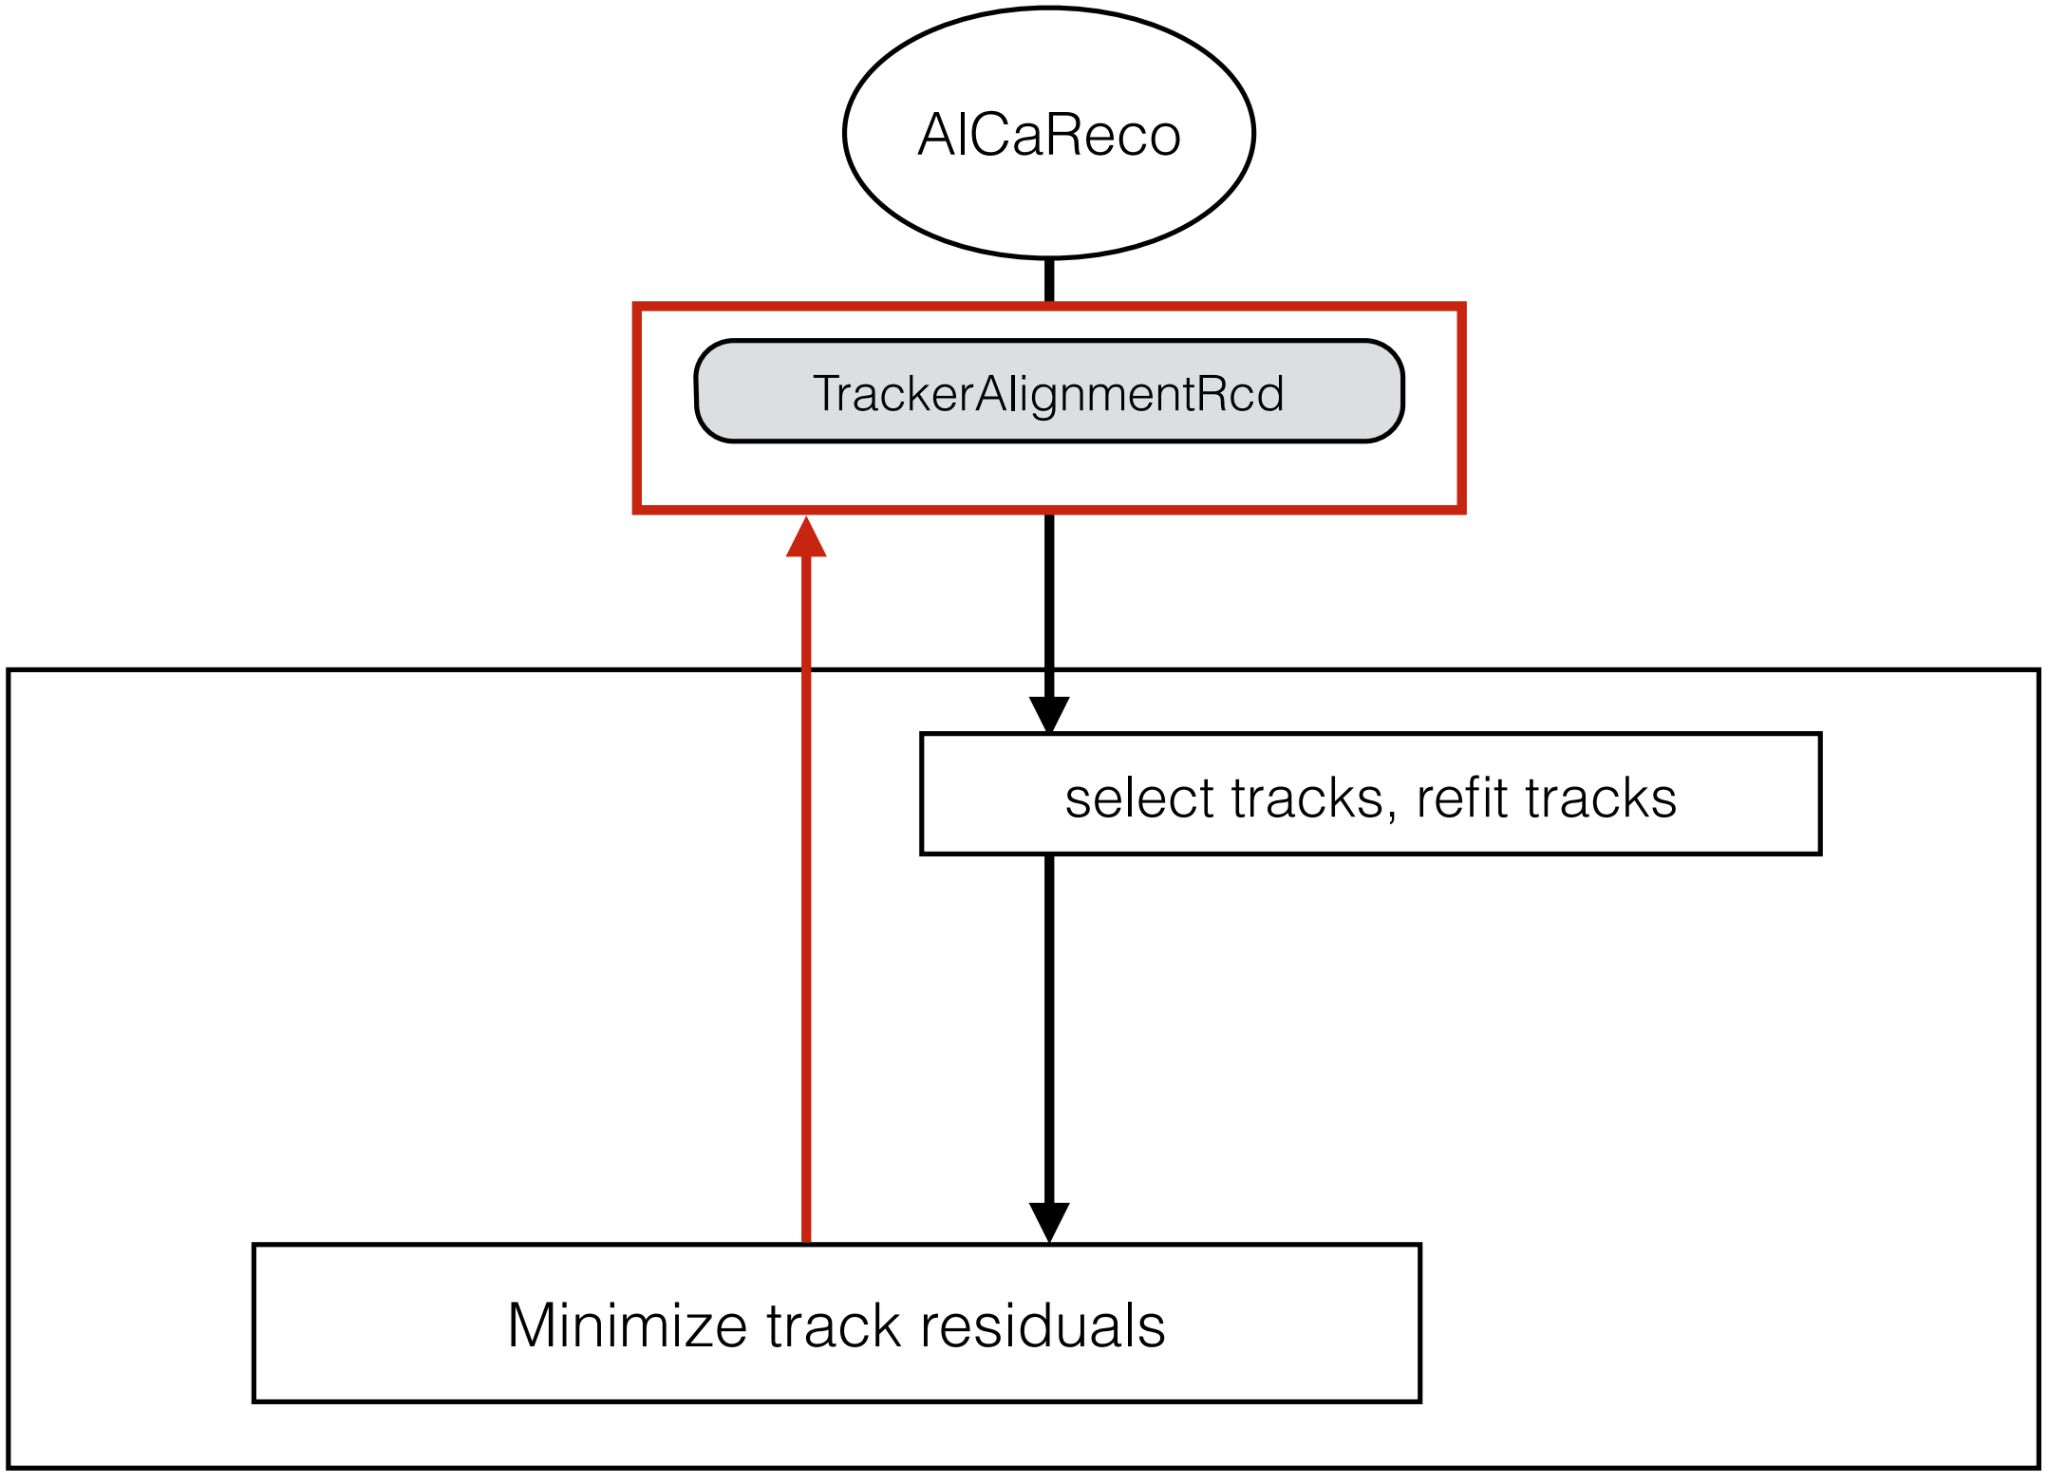
\includegraphics[width=0.8\textwidth,clip] {HIP.jpg}
%         \caption{Process diagram of the Hits-and-Impact-Points (HIP) alignment algorithm \cite{2022166795}.}
%         \label{fig:HIP}
%     \end{center}
% \end{figure}

\subsubsection{HLT alignment at 400\,V}

% Update of HLT conditions triggered by raised HV in BPIX L1 350 → 400 V (Era G) 

% Assisted Millepede team with mp3594.

In late 2022, CMS introduced an updated operational condition in the Barrel Pixel Detector (BPIX), specifically increasing the high voltage (HV) applied to the sensors in Layer 1 from 350\,V to 400\,V, motivated by the cumulative radiation damage experienced by the silicon sensors. 
% This had resulting in degraded charge collection efficiency and overall tracking performance. By elevating the HV, the depletion depth within the sensors was improved, thereby enhancing the signal-to-noise ratio and cluster charge collection efficiency.

However, this HV increase also induced subtle mechanical shifts and modified charge distributions within the pixels, impacting local hit reconstruction. Consequently, the alignment constants utilized by the High-Level Trigger (HLT) required updating to ensure continued accurate track reconstruction at the trigger level. 
% Accurate alignment is critical for maintaining high trigger efficiencies, particularly for vertexing, b-tagging, and lepton-triggering algorithms, all highly sensitive to detector misalignment.

% As part of this update, prompt alignment constants were recalibrated based on data collected immediately following the voltage change. The alignment update underwent thorough validation procedures, employing track-based residuals and Data Quality Monitoring (DQM) tools to assess improvements in track reconstruction accuracy and cluster positioning. Once validated, these updated alignment constants were incorporated into the HLT global conditions database (GT), effectively optimizing the performance of HLT selections during Run~3 Era G data-taking.

% My contribution involved assisting in update of HLT alignment parameters, focusing on the verification of track residual distributions and shifts in the tracker geometry. Using beam data, I prepared a HipPy alternative to the Millepede alignment of the pixel detector at module level while keeping the strips fixed, and ran validation of the new alignment parameters which were then incorporated into the HLT global conditions database (GT), to optimize the performance of trigger selections during Run~3 Era G data-taking~\cite{WeeklyTr24:online}.
My contribution involved assisting in update of HLT alignment parameters, focusing on the verification of track residual distributions and shifts in the tracker geometry. Using beam data, I prepared a HipPy alternative to the Millepede alignment of the pixel detector at module level while keeping the strips fixed, and ran validation of the new alignment parameters which were then incorporated into the HLT global conditions database (GT), to optimize the performance of trigger selections during Run~3 Era G data-taking.

% In December 2022, during Run~3 data-taking (Era~G), the operating high voltage (HV) applied to the innermost layer of the Barrel Pixel Detector (BPIX~L1) was increased from 350\,V to 400\,V. This change was motivated by the need to maintain efficient charge collection in the presence of accumulated radiation damage, particularly affecting the innermost silicon sensors. Higher bias voltages enhance the depletion depth and improve the signal-to-noise ratio, thereby preserving cluster charge and hit reconstruction efficiency critical for robust track seeding.

% This hardware modification had direct implications for the prompt alignment used in the High-Level Trigger (HLT) system. Since the HLT relies on accurate alignment constants to perform online track reconstruction with high efficiency and low fake rates, even minor mechanical shifts—induced by thermal expansion or voltage-related stress—can degrade trigger performance. In particular, the pixel-based tracking algorithms employed at HLT are sensitive to changes in hit positions and cluster shapes, especially for early tracking stages and vertex-based selections.

% To accommodate this change, the Tracker DPG performed an HLT alignment update using data collected after the HV adjustment. Updated alignment constants were derived from track-based residuals and validated through data quality monitoring (DQM) metrics, including hit residuals, track pulls, and pixel hit efficiencies. These constants were subsequently integrated into the HLT Global Tag (GT), ensuring consistent detector geometry across the online and offline reconstruction environments.

% I contributed to this update by assisting in the alignment validation workflow, verifying the compatibility of the updated constants with HLT tracking performance. This included monitoring residual distributions and DQM histograms, and coordinating with the tracker and HLT operations teams to ensure a seamless deployment into the online conditions database. The successful update preserved tracking efficiency across all pixel-based HLT paths, safeguarding the performance of key physics triggers during high-luminosity conditions.

% \begin{figure}[!hbt]
%     \begin{center}
%         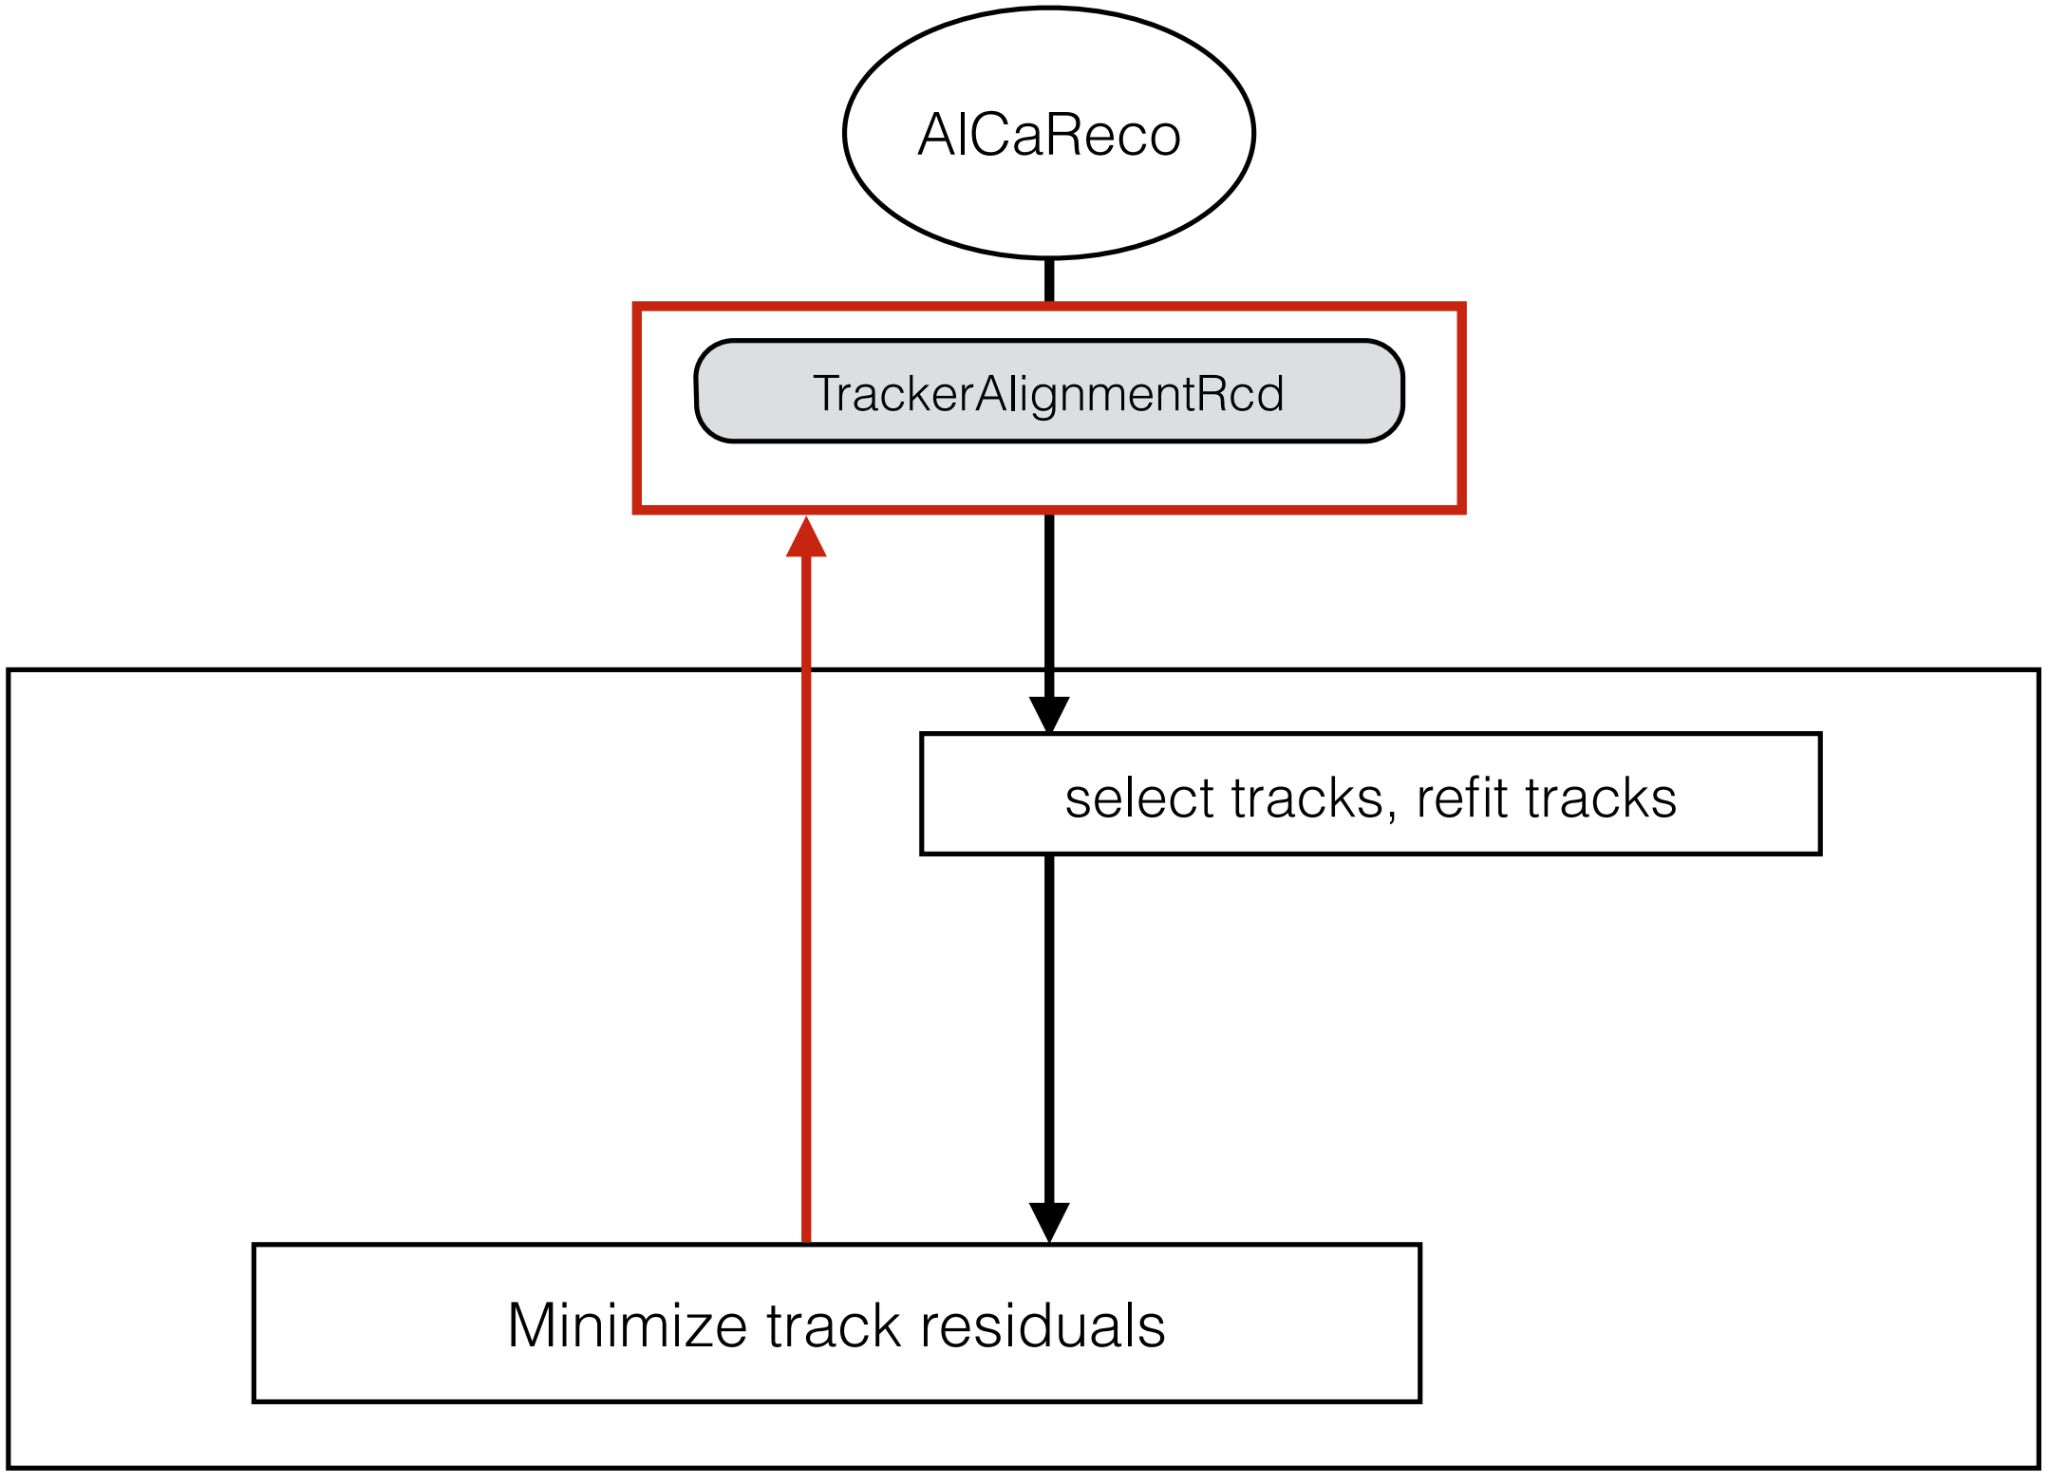
\includegraphics[width=0.8\textwidth,clip] {HIP.jpg}
%         \caption{Process diagram of the Hits-and-Impact-Points (HIP) alignment algorithm \cite{2022166795}.}
%         \label{fig:HIP}
%     \end{center}
% \end{figure}

\subsubsection{2023 Commissioning and Startup}

% I also contributed to the alignment of the tracker during 2023 commissioning and collisions startup. Using early 2023 CRUZET data, I ran a HipPy alignment of the pixel ladder and half-cylinder, as well as the strip HLS (TIB, TOB, TEC)~\cite{Untitled59:online, WeeklyTr66:online}. We were able to match the Millepede alignment of the pixel detector and validated the DMRs for the new alignment parameters, as visualized in Figure~\ref{fig:2023_CRUZET_BPIX}. 
I also contributed to the alignment of the tracker during 2023 commissioning and collisions startup. Using early 2023 CRUZET data, I ran a HipPy alignment of the pixel ladder and half-cylinder, as well as the strip HLS (TIB, TOB, TEC). We were able to match the performance of Millepede for alignment of the pixel detector and validated the DMRs for the new alignment parameters, as visualized in Figure~\ref{fig:2023_CRUZET_BPIX}. 

\begin{figure}[!hbt]
    \begin{center}
        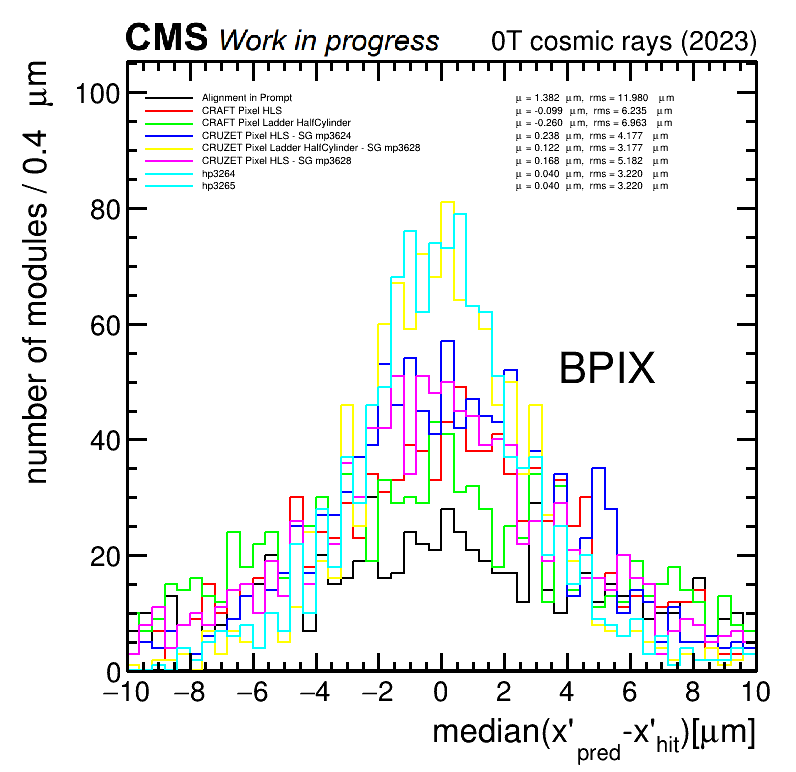
\includegraphics[width=0.9\textwidth,clip] {2023_CRUZET_BPIX.png}
        \caption{Example DMR validation plot for the BPIX, comparing HipPy (cyan) and Millepede (yellow) alignments using early 2023 CRUZET data, both calculated from the starting geometry of mp3628 (green).}
        % ~\cite{WeeklyTr66:online}
        \label{fig:2023_CRUZET_BPIX}
    \end{center}
\end{figure}

% CRAFT 2023 alignment analog to mp3631

% Using mp3628 as SG

% Using cosmics only

% \subsubsection{Investigating HipPy alignment with cosmics}

% \begin{figure}[!hbt]
%     \begin{center}
%         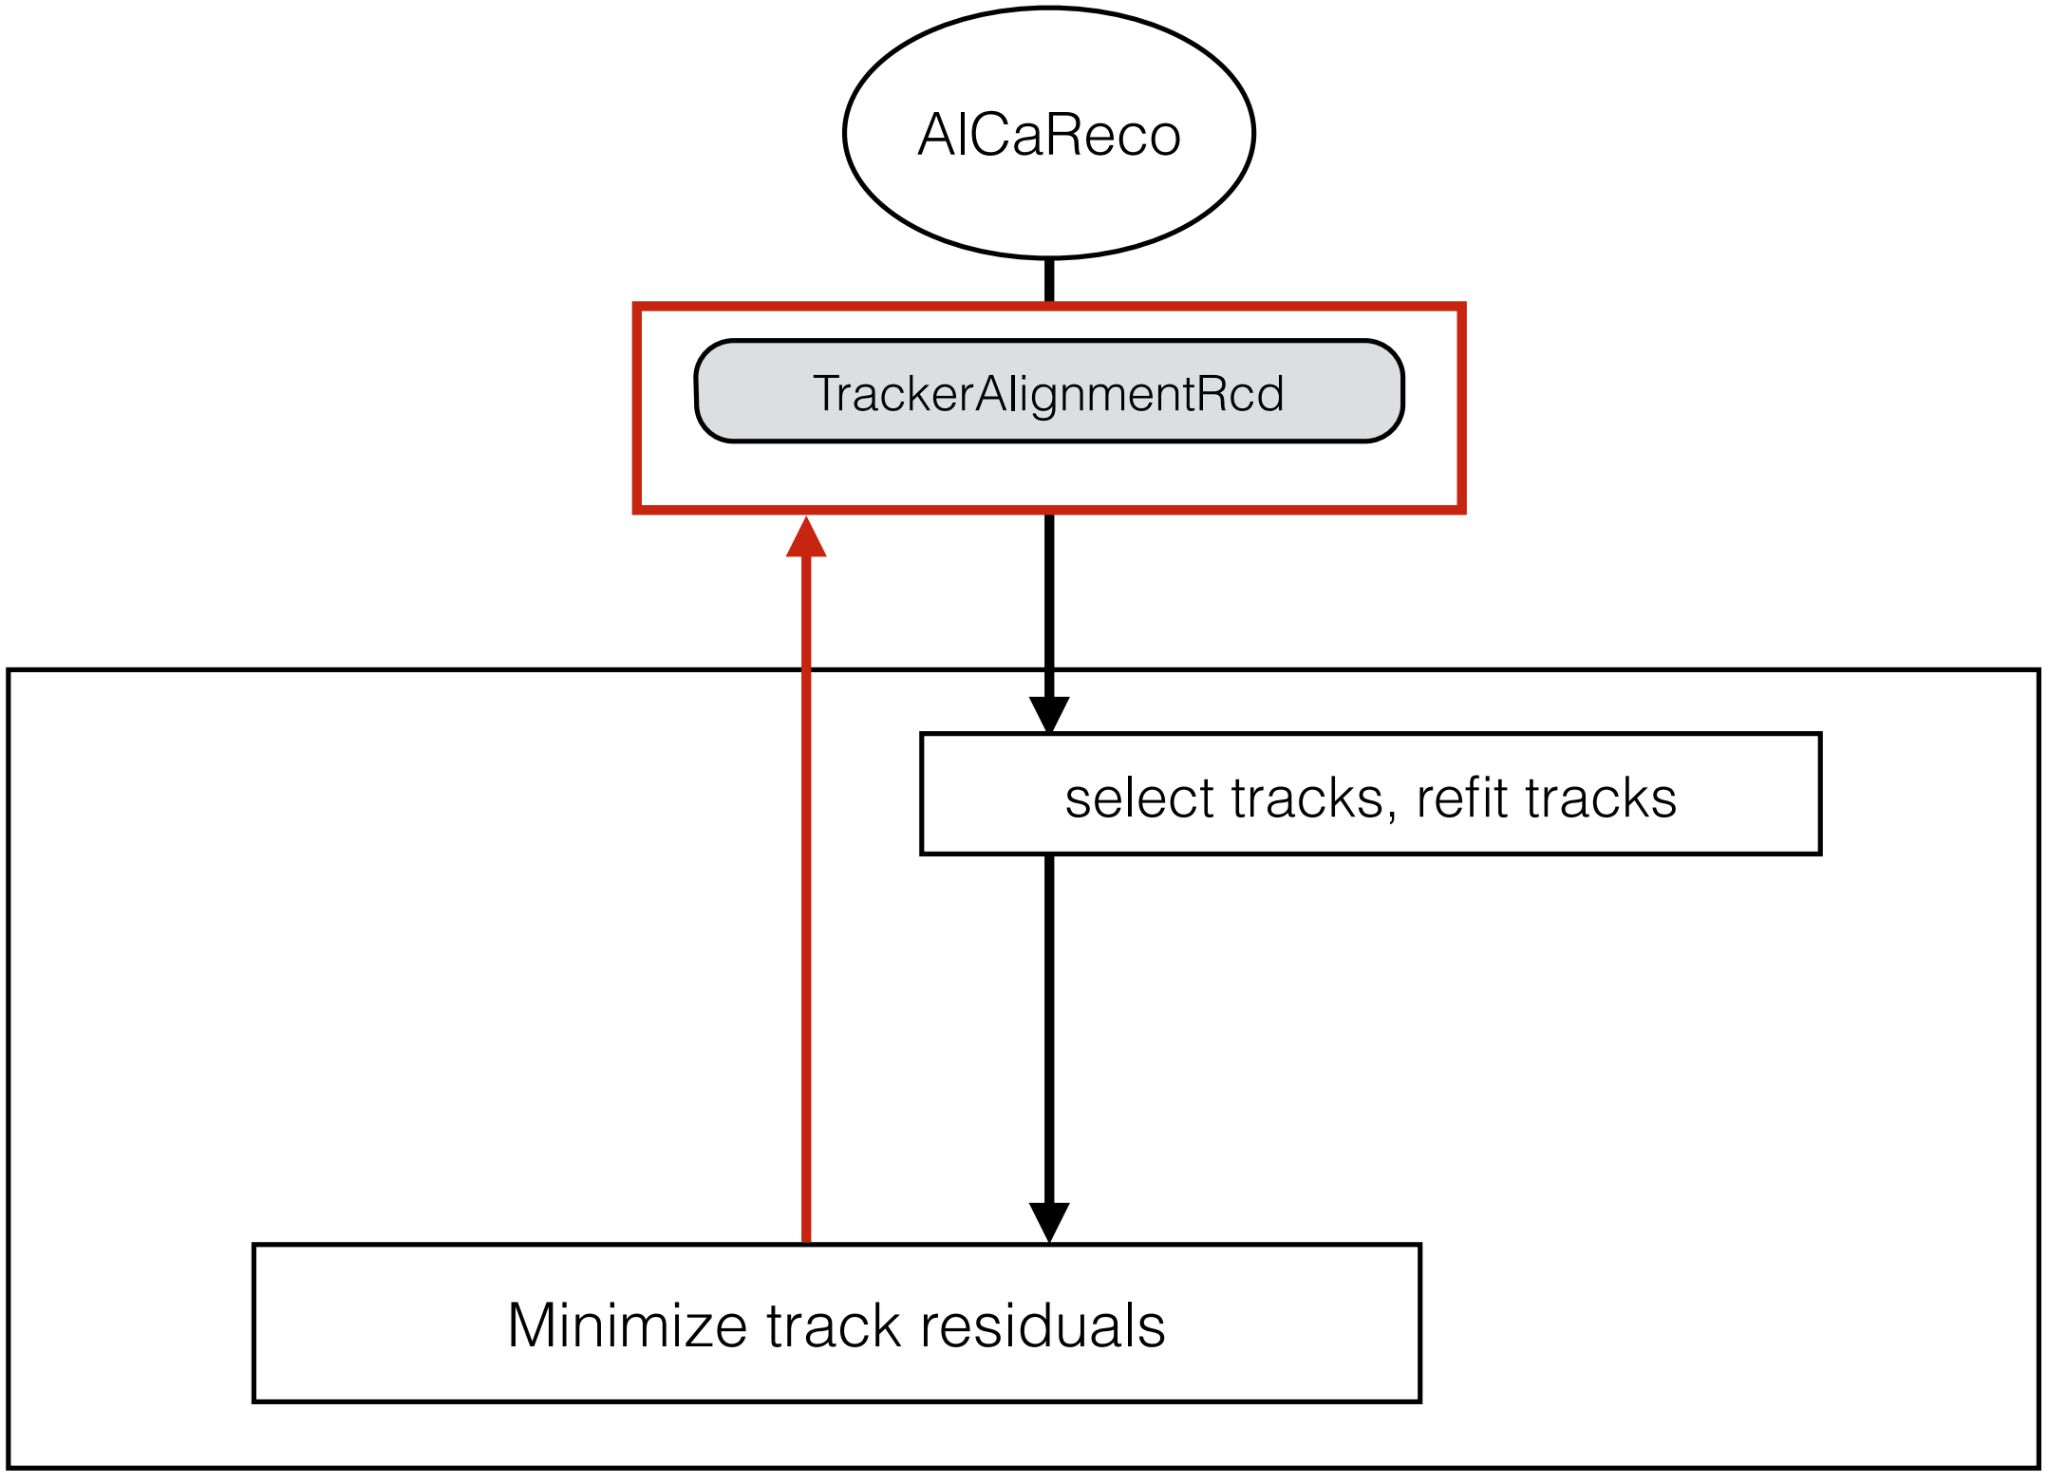
\includegraphics[width=0.8\textwidth,clip] {HIP.jpg}
%         \caption{Process diagram of the Hits-and-Impact-Points (HIP) alignment algorithm \cite{2022166795}.}
%         \label{fig:HIP}
%     \end{center}
% \end{figure}

\subsubsection{Deriving Beam Spot conditions}

The Beam Spot (BS) represents the average interaction region of proton-proton collisions in CMS and serves as a critical reference point for tracking and vertexing. Precise knowledge of the BS position is essential for computing impact parameters, reconstructing primary vertices, and validating alignment parameters. During alignment updates (particularly those affecting the HLT) the most up-to-date beam spot conditions are needed to ensure consistency in the Full Track Validation (FTV), to evaluate the performance of track reconstruction. As part of my contributions to CMS tracker alignment, I derived and plotted BS payloads for several alignment candidates, in collaboration with the Millepede team.

\subsubsection{HipPy Updates}\label{sec:hippyupdates}

% While working with the HipPy algorithm, we have slowly been making upgrades and investigating how to improve its performance for tracker alignment (particularly when using multiple datasets). The latter is still ongoing, but I have been able to modernize the HipPy code to improve functionality and ease of use. Through an update to the official CMS Software (CMSSW) repository, I improved the usability of the codebase by implementing bug fixes and updating the HipPy algorithm to python3. I also modified the HipPy scripts to log additional information about submitted alignment jobs, track ongoing processes without requiring persistent sessions, and avoid interruptions of the algorithm to aid in the execution of more iterations and consequently achieve better alignment performance~\cite{WeeklyTr41:online}. 
While working with the HipPy algorithm, we have been making upgrades and investigating how to improve its performance for tracker alignment (particularly when using multiple datasets). While the latter is ongoing, I have modernized parts of the HipPy code to improve functionality and ease of use. Through an update to the official CMS Software (CMSSW) repository, I improved the usability of the codebase by implementing bug fixes and updating the HipPy algorithm to python3. I also modified the execution scripts to log additional information about submitted alignment jobs, track ongoing processes without requiring persistent sessions, and avoid interruptions of the algorithm to aid in the calculation of more iterations and consequently achieve better alignment performance. 

% I had previously presented the HipPy algorithm at the Second CMS Tracker Alignment Workshop, in preparation for our contributions to tracker alignment in Run~3~\cite{CMSTrack15:online}. After implementing my HipPy updates, I gave a follow-up presentation with a working example of aligning the pixel half-barrel and half-cylinder at the CMS Tracker Training Days~\cite{TrackerT67:online}.
I had previously presented the HipPy algorithm at the Second CMS Tracker Alignment Workshop, in preparation for our contributions to tracker alignment in Run~3. After implementing my HipPy updates, I gave a follow-up presentation with a relevant and interactive example of aligning the pixel half-barrel and half-cylinder at the CMS Tracker Training Days. This alignment campaign calculated new positions for the pixel modules while keeping strips fixed, using a ``MinBias'' dataset---as close as possible to an unbiased sample of recent pp collisions---comprising of 23 million events in this case. Validation plots for the resulting HipPy alignment compared against an analogous Millepede alignment and their shared starting geometry are shown in Figures~\ref{fig:global_tracker_1_final},~\ref{fig:DmedianR_BPIX_plain},~\ref{fig:DmedianR_FPIX_plain},~\ref{fig:DmedianYR_BPIX_plain},~\ref{fig:DmedianYR_FPIX_plain},~\ref{fig:BiasesCanvas_PromptGT_vs_mp3588_vs_hp3252},~and~\ref{fig:BiasesCanvasLayer1_PromptGT_vs_mp3588_vs_hp3252}.
